\documentclass[11pt,letterpaper]{article}

\usepackage{showlabels}
\usepackage{fullpage}
\usepackage{pslatex}
%\usepackage{latexsym}
\usepackage[english]{babel}
\usepackage[utf8]{inputenc}
\usepackage{amsmath}
\usepackage{bm}
\usepackage{graphicx}
\usepackage{tikz}
\usepackage{xcolor}
\usepackage{url}
%\usepackage[colorinlistoftodos]{todonotes}
\usepackage{rotating}
\usepackage{natbib}
\usepackage{amssymb}

\usepackage{tikz-dependency}
\usepackage{longtable}


\newcommand{\R}[0]{\mathbb{R}}
\newcommand{\E}[0]{\mathbb{E}}
\newcommand{\Ff}[0]{\mathcal{F}}

\usepackage{multirow}

\newcommand{\soft}[1]{}
\newcommand{\nopreview}[1]{}
\newcommand\comment[1]{{\color{red}#1}}
\newcommand\mhahn[1]{{\color{red}(#1)}}
\newcommand\note[1]{{\color{red}(#1)}}
\newcommand\jd[1]{{\color{red}(#1)}}
\newcommand\rljf[1]{{\color{red}(#1)}}
\newcommand{\key}[1]{\textbf{#1}}

\usepackage{amsthm}

\newcommand{\thetad}[0]{{\theta_d}}
\newcommand{\thetal}[0]{{\theta_{LM}}}

\newcounter{theorem}
\newtheorem{proposition}[theorem]{Proposition}
\newtheorem{thm}[theorem]{Theorem}
\newtheorem{corollary}[theorem]{Corollary}
\newtheorem{question}[theorem]{Question}
\newtheorem{example}[theorem]{Example}
\newtheorem{lemma}[theorem]{Lemma}


\frenchspacing
%\def\baselinestretch{0.975}

%\emnlpfinalcopy
%\def\emnlppaperid{496}

\title{Crosslinguistic Word Orders Enable an Efficient Tradeoff between Memory and Surprisal}
\author{Michael Hahn, Judith Degen, Richard Futrell}
\date{2018}

\begin{document}

\maketitle


\begin{abstract}
Online memory limitations are well-established as a factor impacting sentence processing and have been argued to account for crosslinguistic word order regularities. Building off expectation-based models of language processing, we provide an information-theoretic formalization of these memory limitations. We introduce the idea of a memory-surprisal tradeoff: comprehenders can achieve lower average surprisal per word at the cost of storing more information about past context. We show that the shape of the tradeoff is determined in part by word order. In particular, languages will enable more efficient tradeoffs when they exhibit information locality: when predictive information about a word is concentrated in the word’s recent past. We show evidence from corpora of 52 real languages showing that languages allow for more efficient memory-surprisal tradeoffs than random baseline word order grammars. 
\end{abstract}


 
\section{Introduction}



%Each human language is a system for encoding an infinite variety of thoughts into sentences, i.e. linear strings of words.
%A primary goal of the field of linguistics is to characterize and explain the commonalities and differences among these systems, and so to gain insight into the cognitive machinery that underpins this fundamental aspect of human intelligence.
Why is human language the way it is? 
In this paper, we argue that the grammars of human languages can be modeled mathematically as solutions to the problem of maximally efficient communication among agents subject to particular resource constraints on information processing during speaking and listening.
We formalize these constraints using information theory.
Using these concepts, we show novel large-scale quantitative evidence from 54 languages that information is structured in time so as to minimize memory load during language comprehension, and
we show that our formalization allows us to explain some of the universal syntactic properties of languages.

The suggestion that the structure of human language reflects a need for efficient processing under resource limitations has been present in the theoretical and functional linguistics literature for decades~\citep{yngve1961,berwick1984grammatical,hawkins1994performance,jaeger2011language,gibson2019efficiency}, and has been summed up in \citeauthor{hawkins1994efficiency}'s (\citeyear{hawkins1994efficiency}) \key{Performance--Grammar Correspondence Hypothesis} (PGCH), which holds that grammars are structured so that the typical utterance is easy to produce and comprehend under performance constraints.
The idea has also been controversial, with prominent claims that efficiency in this sense has had no or only a minimal effect on the structure of human language \citep{chomsky}.

Among theories of language based on processing efficiency, some of the most successful have been those dealing with resource constraints on working memory as deployed during language production and comprehension.
An extensive body of work from psycholinguistics has documented that limitations in incremental memory cause measurable difficulty in production and comprehension \citep{gibson1998syntactic,gibson1999memory,gibson2000dependency,lewis2005activationbased,bartek2011search,nicenboim2015working}. % TODO are there cites for production?
Complementing this work, a number of researchers in linguistic typology and corpus linguistics have shown how various universal properties of grammars can be explained in terms of memory-based processing difficulty \citep{hawkins2004efficiency,hawkins2014crosslinguistic,ferrericancho2006syntactic,gildea2010grammars,futrell2015largescale,liu2017dependency,temperley2018dependency}.
We will see that one of the most successful theories in this domain, the principle of \key{dependency length minimization}, falls out of our formalization of processing efficiency as a special case.
%Our work formalizes and generalizes this previous work.

We formalize the notion of memory constraints in language processing in terms of what we call the \key{memory--surprisal tradeoff}: the idea that it is possible to achieve greater ease of word-by-word comprehension, and greater accuracy in word-by-word production, at the cost of investing more computational resources into remembering previous words.
The shape of this tradeoff depends on the grammar of a language, and in particular its word order properties.
We characterize memory resources in a theory-neutral, information-theoretic manner based on rate--distortion theory \citep{cover2006elements} and the theory of statistical complexity \citep{crutchfield1989inferring}. % cite the crutchfield nature review, and predictive info bottleneck


%For each amount of memory invested, a language permits a certain level of ease of processing 
%The resulting tradeoff of memory and surprisal of depends on the word order properties of a language. Analogous results also hold for language production by resource-constrained speakers. We show evidence that the preferred word orders of natural languages are those that enable efficient memory--surprisal tradeoffs.

The remainder of this paper is structured as follows. In Section~\ref{sec:background}, we give a brief review of previous work on the effects of short-term memory on languages and language processing. In Section~\ref{sec:ms-tradeoff}, we describe the memory--surprisal tradeoff and how it results from rate--distortion theory, the theory of optimal information processing under resource constraints \citep{cover2006elements}. In Section~\ref{sec:info-locality}, we prove that word orders enable efficient processing in terms of the memory--surprisal tradeoff when they exhibit \emph{information locality}: whenever utterance elements that predict each other are close to each other. In Section~\ref{sec:experiment1}, languages which have previously been shown to be preferred in artificial language experiments are exactly those that enable efficient memory--surprisal tradeoffs \citep{fedzechkina2017human}. In Section~\ref{sec:experiment2}, we show that word orders of natural languages as found in dependency corpora \citep{ud} enable more efficient memory--surprisal tradeoffs than baseline word orders. Section~\ref{sec:conclusion} concludes.


%These strategies can be seen as sets of rules that differ in the way ...
%Languages differ considerably in the rules they apply to order information: English orders the object after the verb, Japanese places it before the verb \note{make more explicit here}.
%Explaining the variation in the strategies languages use to  order underlying hierarchical structures into linear strings of words has been one of the foci of linguistic research (\jd{CITE}).
%We show that these strategies reflect an underlying optimization principle: human languages are adapted to limitations in human working memory.

%We test the hypothesis that human languages represent different solutions to the problem of efficient computation with constrained working memory.






%\mhahn{original intro}
%Since the 1950s, it has been a persistent suggestion that human language processing is shaped by a resource bottleneck in short-term memory.
%Language is produced and comprehended incrementally in a way that crucially requires both speaker and listener to use an active memory store to keep track of what was previously said.
%Since short-term memory of this kind is known to be highly limited in capacity \citep{miller1956magical}, it makes sense for these capacity limits to comprise a major constraint on production and comprehension.
%Indeed, a great deal of work in sentence processing has focused on characterizing the effects of memory constraints on language processing \citep{gibson-linguistic-1998,lewis-activation-based-2005,levy2013memory}.

%At the same time, the field of functional linguistics has argued that these resource constraints not only affect online language processing, they also shape the form of human language itself.
%For example, the Performace--Grammar Correspondence Hypothesis (PGCH) of \citet{hawkins1994performance} holds that forms which are practically easier to produce and comprehend end up becoming part of the grammars of languages, and that this process can explain several of the universal properties of human languages originally documented by \citet{greenberg-universals-1963}.







\section{Background}\label{sec:background}
% More detailed lit review

A wide range of work has argued that natural language orders information in ways that reduce memory effort.
An early example is \cite{miller-finitary-1963}, who attributed the unacceptability of multiple center embeddings in English to limitations of human working memory.
\cite{hawkins-efficiency-2003} provides cross-linguistic evidence that word orders are optimized for processing based on local contexts.
Further work has found computational, corpus-based evidence that memory limitations impact language structure and production.
In particular, languages have been shown to shorten the length of syntactic dependency lengths \citep{futrell-large-scale-2015}.
Dependency length can be linked to memory use in certain models of incremental syntactic parsing, and increases processing difficulty in theories of memory in sentence processing \citep{gibson-linguistic-1998}.
\cite{gildea-human-2015} further provide evidence from five languages that word orders optimize predictability from local contexts.
\cite{futrell-noisy-context-2017} provide evidence that language shows information locality, i.e., elements with higher mutual infomation are closer together, which is predicted by their model of Lossy-Context Surprisal.

All these models of memory in sentence processing, and derived measures of efficiency for memory allocation, require specific assumptions about the architecture of memory.
This leaves open the question whether such assumptions are necessary, or whether word orders across languages are optimized for memory independently of the implementation and architecture of human language processing.


We approach this question by first providing general information-theoretic lower bounds on memory load that will hold independently of the architecture of memory representations.
We will consider a general setting of a listener performing incremental prediction.
Our result immediatly entails a link between boundedness of memory and locality, which had been stipulated or derived from assumptions about memory architecture in previous models \citep{gibson-linguistic-1998, lewis-activation-based-2005, futrell-noisy-context-2017}.
We will then use corpus data from over 52 languages to provide evidence that their word orders help lower memory cost.

%TODO mention prior work
%
%-  center embeddings dispreferred/impossible to process \cite{miller-finitary-1963}
%
%- explanation of greenberg universals
%
%- dependency length minimization
%
%- \cite{gibson-linguistic-1998}
%

%\paragraph{\cite{berwick-grammatical-1986}}
%They considered incremental parsing, or, more precisely, incremental recognition of grammaticality.



%also (CITE): operations in a specific incremental parsing model





\section{Memory-Surprisal Tradeoff}\label{sec:ms-tradeoff}


%We consider a \emph{listener} who, as the speaker's utterance unfolds, engages in incremental prediction.
%%Informally, we expect that both speaker and listener will be affected by memory demands:
%%rom the speaker's perspective, producing well-formed sentences will require information about what she has uttered so far.
%For the listener, predicting the next word well requires maintaining information about the past.
%For the listener, the quality of prediction is measured by the average \emph{surprisal} experienced.
%For a fixed language, we can ask how much information about the past (1) the speaker has to maintain to produce well-formed utterances, and (2) the listener has to maintain to incur a minimal amount of surprisal.
%Utilizing the tools of information theory, we quantify memory in \emph{bits}, obtaining bounds that hold across different models of memory architecture and ways of quantifying memory load.
%
%
%TODO say at some point that we're studying sentence-internal memory



\begin{figure}
\centering
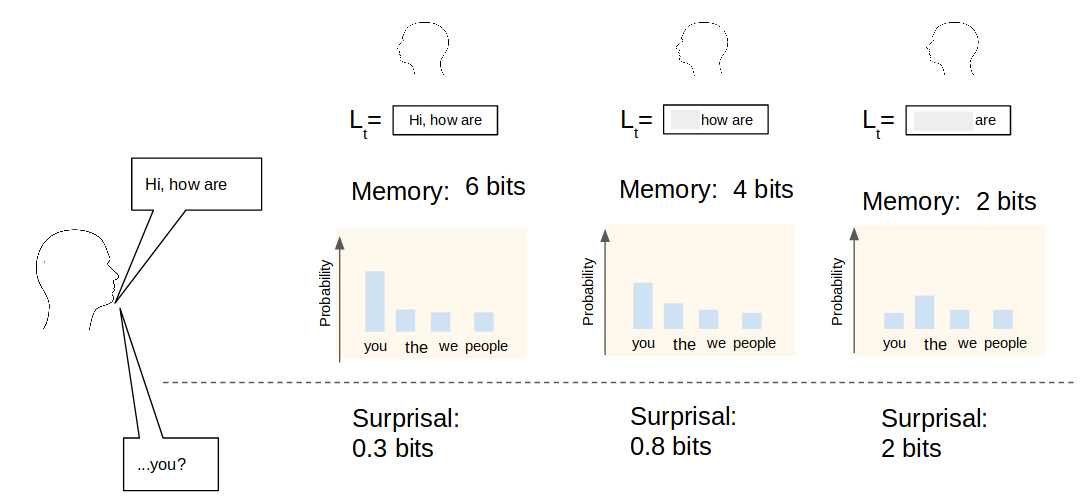
\includegraphics[width=0.9\textwidth]{figures-gdrive/communication.png}
	\caption{Memory and language comprehension. (1) A speaker produces a sequence of words. (2) A listener maintains a representation of the words received so far. The listener can represent these at higher (left) or lower (right) levels of precision. (3) Throughout communication, the listener generates probabilistic expectations about the next word. Higher precision of memory representations leads to more precise predictions. (4) When receiving the next word, the listener incurs surprisal depending on the predictions. Higher levels of fidelity in memory lead to lower surprisal on average. \jd{what do the numbers (1) (2) etc refer to? also: image is blurry, at least on my screen}\note{make reference to $L_t$ inside the caption. you and the surprisals visually better aligned. maybe can color-code? } \mhahn{problem suggests that memory has to be contiguous substrings}}
	\label{fig:communication}
\end{figure}

We begin developing our model by considering the process of language comprehension illustrated in Figure~\ref{fig:communication}, where the listener Alice is processing a stream of words uttered by an interlocutor Bob (Figure~\ref{fig:communication}).


Experimental research has established that (1) listeners maintain information about the words received so far, (2) listeners forms probabilistic expectations about the upcoming words, and (3) words are easy to process to the extent that they are predictable in context \rljf{Good source for other cites here would be to dig around in Luke \& Christianson's review of predictability effects}. Furthermore, the exact mathematical form of the relationship between predictability and processing difficulty (as measured e.g. in reading times) seems to be given by the \key{information content} of a word in context \cite{hale2001probabilistic,levy2008expectation,smith2013effect}.


Surprisal theory \citep{hale-probabilistic-2001, levy-expectation-based-2008} posits that the processing effort on a word $w_t$ in context $w_1\dots w_{t-1}$ is proportional to the \key{surprisal} of the word in context:
\begin{equation}
S = -\log \operatorname{P}(w_t|w_1\dots w_{t-1})\label{eq:surp}.
\end{equation}
Experimental work has confirmed that surprisal is a reliable and linear predictor of processing effort as reflected in reading times \citep{smith-effect-2013}.

The average processing difficulty associated with a language then comes out to its entropy rate:
\begin{equation}
	S = \operatorname{H}(w_t|w_1\dots w_{t-1}).
\end{equation}



However, surprisal theory as presented above cannot in principle account for effects of memory limitations on online processing, because Equation~\ref{eq:surp} represents surprisal as experienced by an idealized listener who accurately remembers the entire history of previous words $w_{1...t-1}$.
More realistically, human listeners deploy memory resources that maintain imperfect representations of the preceding context \citep{lewis-activation-based-2005, futrell-noisy-context-2017}.
If $m_{t-1}$ is a listener's memory state after hearing $w_1\dots w_{t-1}$, then the true surprisal experienced by the listener will be:
\begin{equation}
  \label{eq:lossy-surp}
  S_M := -\log_2 \operatorname{P}(x_t|m_{t-1}),
\end{equation}
which must be larger than Eq.~\ref{eq:surp} on average (see below for proof).
This modified surprisal $S_M$ in Eq.~\ref{eq:lossy-surp} can account for well-known memory effects on online processing such as dependency locality effects and structural forgetting \citep{futrell-noisy-context-2017,futrell2019information}.
The limitations of memory have well-documented empirical effects on language processing, causing difficulty above and beyond the difficulty associated with raw information content \cite{gibson1998linguistic,gibson1999memory,gibson2000dependency,vasishth2005activationbased,levy2013memory}.

The average processing difficulty associated with a language then comes out to a \key{cross entropy}:
\begin{equation}
	S = \operatorname{H}(w_t|m_{t-1}).
\end{equation}


These considerations imply a \emph{tradeoff between memory and surprisal}:
A listener maintaining higher-precision memory representations $m_{t-1}$ will, on average, incur lower surprisal, at the cost of higher memory load.
The idea of the memory-surprisal tradeoff is visualized in Fig.~\ref{fig:tradeoff}: for each desired level of average surprisal, there is a minimum number of bits of information which must be stored about context.
The shape of the trade-off is determined by the language, and in particular its word order:
some languages enable more efficient trade-offs than others by forcing a listener to store more bits in memory to achieve the same level of average surprisal.


Here we propose to model human language comprehension by treating the listener's memory $m_{i-1}$ as a lossily compressed representation of the context $x_{1...i-1}$, and the processing effort associated with each word using Eq.~\ref{eq:lossy-surp}.
Suppose that the listener's memory has a fixed information-carrying capacity $k$, then this listener has to compress the context into a memory representation $m_{i-1}$ with at most $k$ bits: $H[m_{i-1}] \leq k$.
Information theory implies that the processing cost $S_M$ trades off with the memory capacity $k$:
Processing cost will be lower for a listener who represents past input at higher levels of precision.




We prove a theorem describing how the shape of this tradeoff relates to language structure. %relating memory to the experienced comprehension difficulty $S$.
%Informally, the theorem says that languages support more efficient tradeoffs between short-term memory and comprehension difficulty when words are strongly predictive of their neighboring words.
This theorem captures formally that languages support more efficient tradeoffs between short-term memory and comprehension difficulty when words are strongly predictive of their neighboring words.


We derive the precise form of the memory-surprisal tradeoff in Theorem 1.
Let $\operatorname{I}_t$ be the conditional mutual information between words that are $t$ steps apart, conditioned on the intervening words: 
\begin{equation}
	\operatorname{I}_t := \operatorname{I}[w_t, w_0 | w_1, \dots, w_{t-1}] = \operatorname{H}[w_t|w_1, \dots, w_{t-1}] - \operatorname{H}[w_t|w_0, \dots, w_{t-1}] 
\end{equation}

This quantity measures how much predictive information the word $t$ steps in the past contains about the current word, above and beyond the information contained in the intervening words.

This is equal to the reduction in uncertainty about the $t$-th observation when knowing the $0$-th observation, in addition to the block of intervening observations.
That is, we measure the amount of statistical dependency of observations that are $t$ steps apart, controlling for any information that is redundant with intervening observations.
This quantifies how much information needs to be carried across $t$ timesteps without any possibility for `guessing' it from intervening observations.

This quantity, visualized in Figure~\ref{fig:theorem} (a), measures how much predictive information is provided by the next word $w_t$ by the word $t$ steps in the past.
It is a statistical property of the language, and can be estimated from large-scale text data.


Our theoretical results describe how the tradeoff between memory and comprehension difficulty relates to $I_t$ (Figure~\ref{fig:theorem} (b)):
Consider a listener who invests $B$ bits of memory into representing past input.
We then consider the smallest $T$ such that the area under the curve of $t I_t$, to the left of $T$, has size $B$.
Such a listener will experience average surprisal at least $H[w_t| w_{<t}] + \sum_{t=T+1}^\infty I_t$. %\note{maybe result first, and then say what $T$ is}
By tracing out all values $T >0$, one can obtain a bound on the tradeoff curve for any possible listener.

This is formalized in the following theorem:

\begin{thm}\label{prop:suboptimal}
Let $T$ be a positive integer, and consider a listener using at most $\sum_{t=1}^T t \operatorname{I}_t$ bits of memory on average.
Then this listener will incur average surprisal at least
$\operatorname{H}[w_t|w_{<t}] + \sum_{t > T} \operatorname{I}_t$.
\end{thm}


We provide a rigorous proof, making only minimal mathematical assumptions, in Appendix Section X.

An intuitive (non-rigorous) argument for this theorem goes as follows:
For each bit of information that is held in memory, we count the number of timesteps from when it is first entered into memory to when it is forgotten.
If a word $w_{T-t}$, $t$ steps in the past, contains one bit of information about the current word $w_T$, and if this information is not redundant with information in the intervening words, then this bit of information had to be maintained in memory for $t$ steps.
The amount of such information is $I_t$. This explains the factor $t$.


The theorem allows us to estimate the extra surprisal associated with each amount of memory capacity for a language.
The quantities $\operatorname{I}_t$ can be estimated as the difference between the cross-entropy of language models that have access to the last $t-1$ or $t$ words.
Given such estimates of $\operatorname{I}_t$, we estimate tradeoff curves as in Figure~\ref{fig:tradeoff} by tracing out $T=1, 2, \dots$.


Our result is entirely information-theoretic and applies to \emph{any} physical encoding of the past, entirely independent of the implementation of the model. % and the mechanisms by which it computes predictions.
In particular, while the relation to psycholinguistic and psychological models of how memory works will be interesting to explore, our result applies to any such model.
Memory representations do not have to be rational or optimal for this bound to hold:
It provides a \emph{lower bound} on the amount of information that needs to be stored -- other memory representations will always need to store at least as much information.








\begin{figure}
	(a)
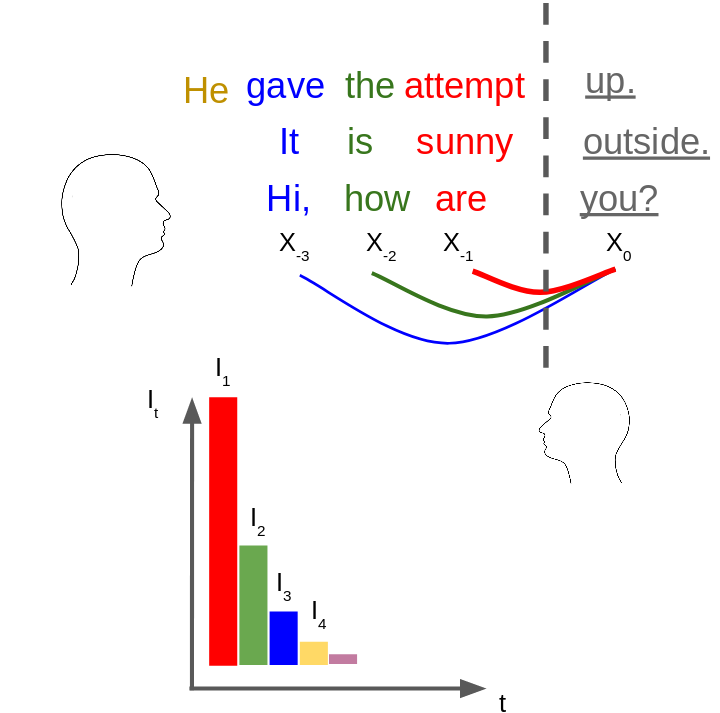
\includegraphics[width=0.4\textwidth]{figures-gdrive/mi-distance.png}
	(b)
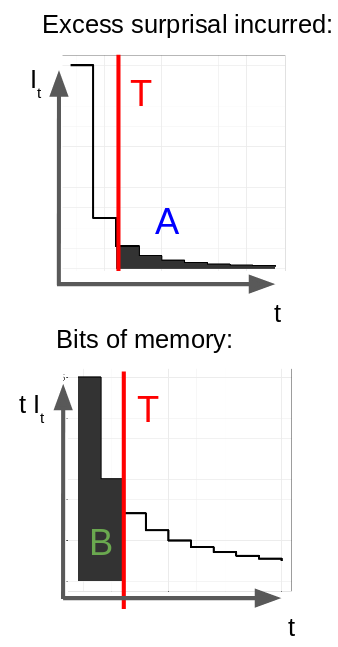
\includegraphics[width=0.2\textwidth]{figures-gdrive/theorem.png}
	(c)
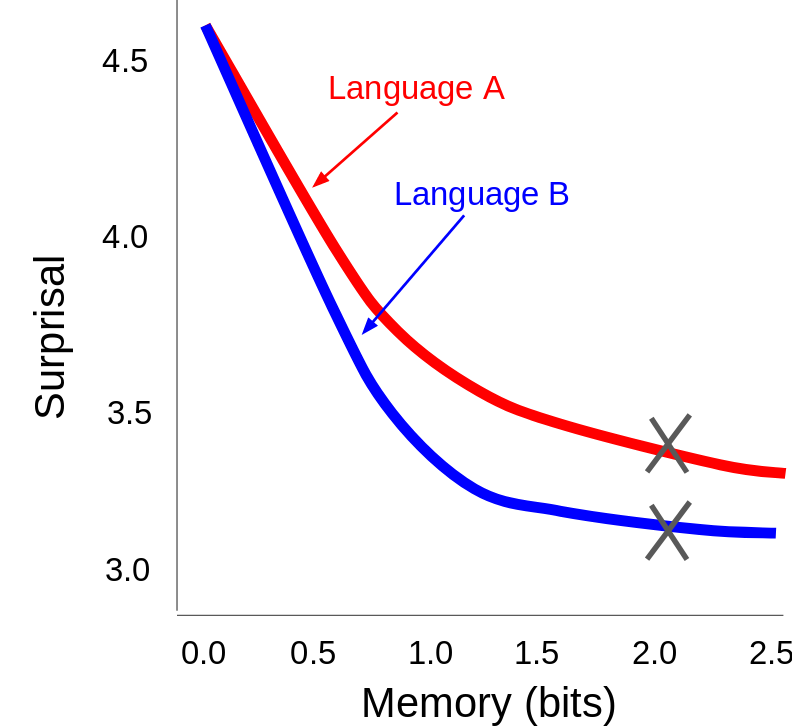
\includegraphics[width=0.2\textwidth]{figures-gdrive/tradeoff.png}
	\caption{
		(a) Conditional mutual information $I_t$ captures how much predictive information about the next word is provided, on average, by the word $t$ steps in the past.
		(b) Here we illustrate our theoretical result. We plot $I_t$ (top) and $tI_t$ (bottom) as functions of $t$. A listener using $B$ bits memory (bottom) to represent prior observations will incur at least $A$ bits of extra surprisal beyond the entropy rate (top). \note{there is t and T. COnfusing}
		(c) \jd{FILL OUT} \note{make the colors in (c) difefrenfr from this in (b). Do want to make clear what the mapping from (b) to (c) is. Maybe can even have a pair of the two (b) curves, and then show what they map on.}
}\label{fig:theorem}
\end{figure}


%TODO
%Let $I_t$ be the Conditional Mutual Information of two words $w_0, w_t$ conditioned on the intervening words:
%\note{hard to swallow for general audience. maybe can just use more straightforward less mathy language.}
%
%
%\note{Alternative:}
%A listener will experience average surprisal at least
%\begin{equation}
%	H[w_t| w_{<t}] + \sum_{t=T+1}^\infty I_t
%\end{equation}
%where $T$ is chosen to be the smallest $T$ for which $\sum_{t=1}^T t I_t \geq B$.
%\note{End alternative.}


%We prove that, for any integer $T > 0$, a listener encoding $\sum_{t=1}^T t I_t$ bits of memory will incur average surprisal at least $H[w_t| w_{<t}] + \sum_{t=T+1}^\infty I_t$.
%maybe multiple sentences in def of It?
%define math, AND give people intuition.





\begin{figure}
\centering
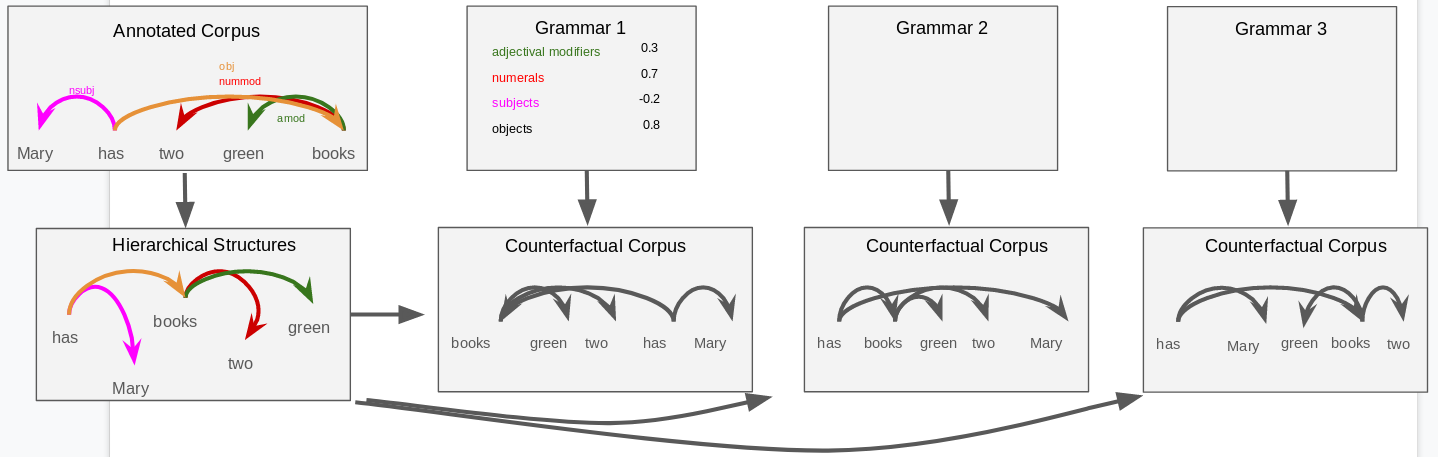
\includegraphics[width=\textwidth]{figures-gdrive/counterfactual-languages.png}
	\caption{\note{Can say more here to explain how it works} Estimating chance by constructing counterfactual grammars and languages.\jd{this figure is again blurry for me. also looks like there's sth in the background on the left?}}\label{fig:grammars}
\end{figure}










We now introduce our main theoretical result on memory-surprisal tradeoffs.





\begin{figure}
	\begin{center}
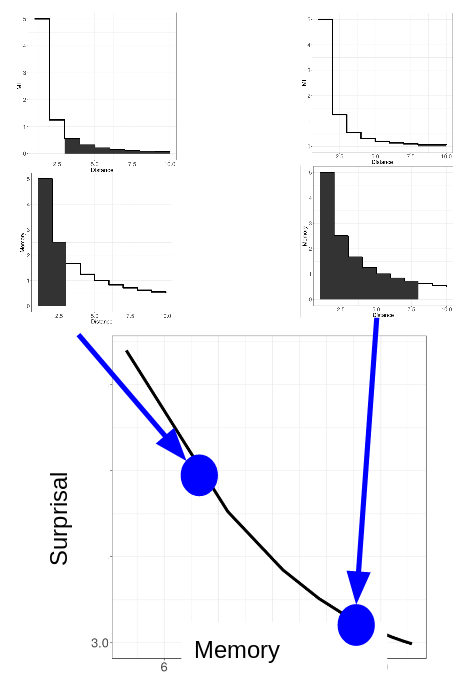
\includegraphics[width=0.45\textwidth]{figures/interpolate-curve.png}
\end{center}
	\caption{Estimating memory-surprisal tradeoff using the Theorem: We trace out the memory and surprisal values for all $T=1, 2, ...$, and linearly interpolate the curve.}\label{fig:interpolate}
\end{figure}







The proposition gives us a lower bound on the listener's memory-surprisal curve: Taking all pairs of memory $\sum_{t=1}^T t I_t$ and surprisal $H[w_t|w_{<t}] + \sum_{t > T} I_t$.
Then interplate linearly (justify this in appendix).
We obtain a curve in memry-surprisal plane, which is a lower bound on the memory demands of any listener at a given surprisal level.
We visualize this for the two processes from Figure~\ref{fig:basic} in Figure~\ref{fig:listener-tradeoff}.


\begin{figure*}
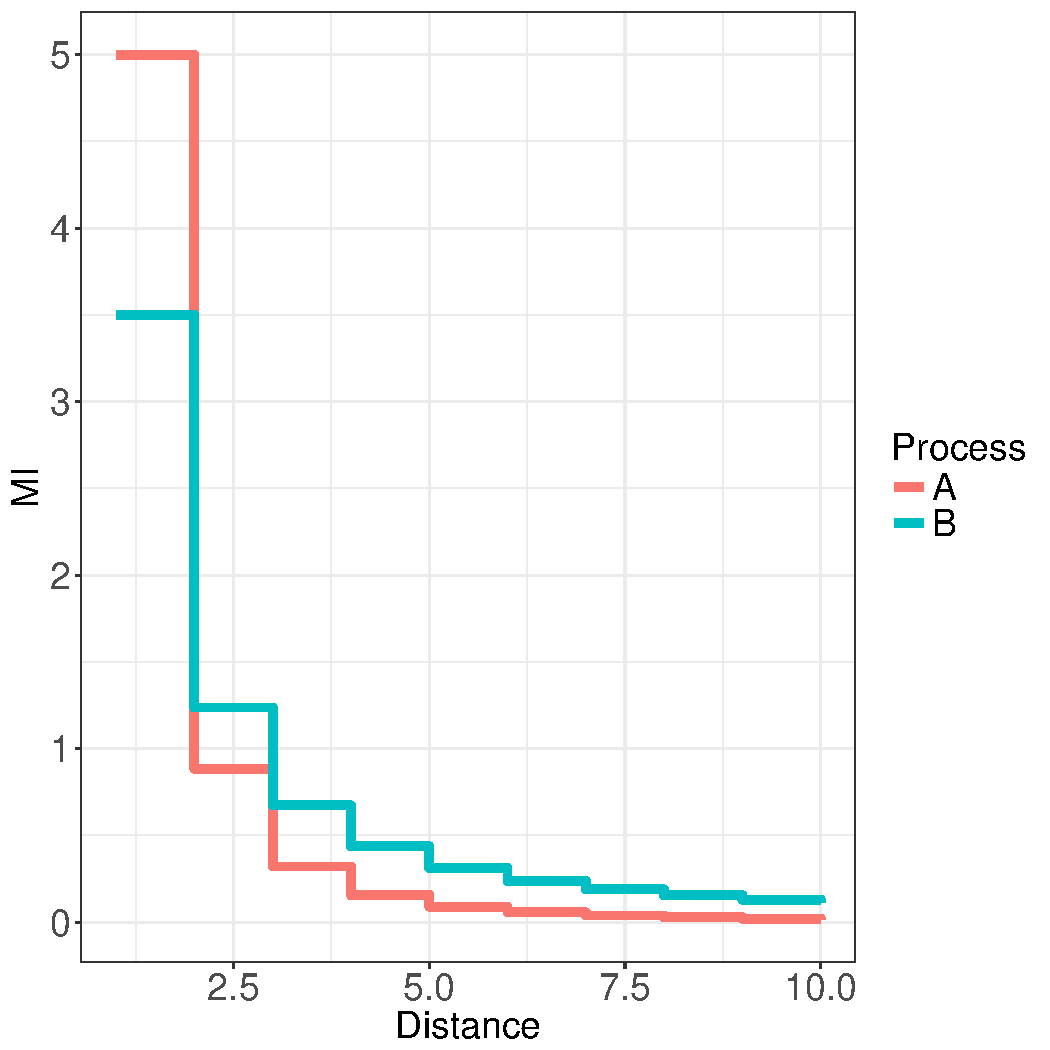
\includegraphics[width=0.45\textwidth]{../code/toy/figures/decay.pdf}
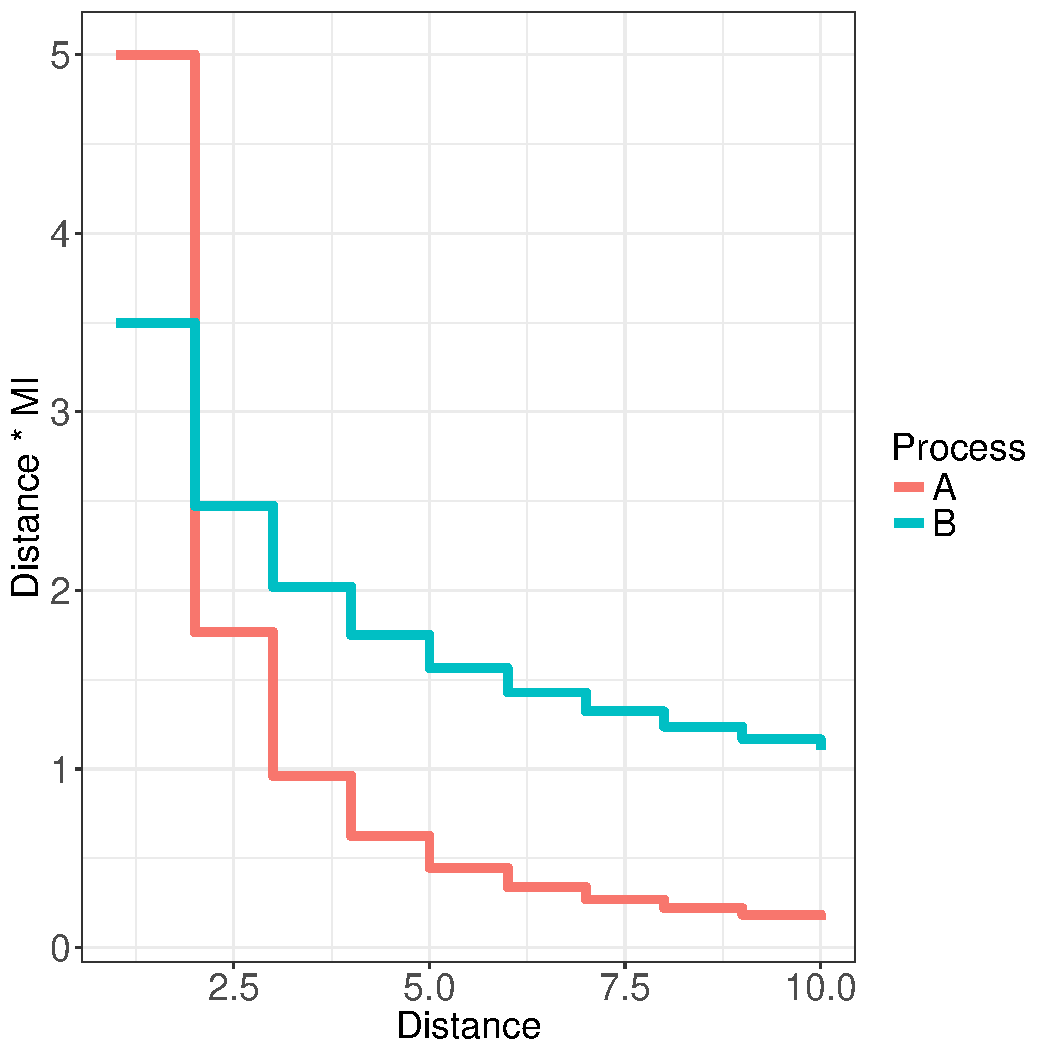
\includegraphics[width=0.45\textwidth]{../code/toy/figures/memory.pdf}
%
	\caption{Left: $I_t$ as a function of $t$, for two different processes. $I_t$ decays faster for the red process: Predictive information about the present observation is concentrated more strongly in the recent past. Left: $t \cdot I_t$ as a function of $t$ for the same processes. }\label{fig:basic}
\end{figure*}



\begin{figure}
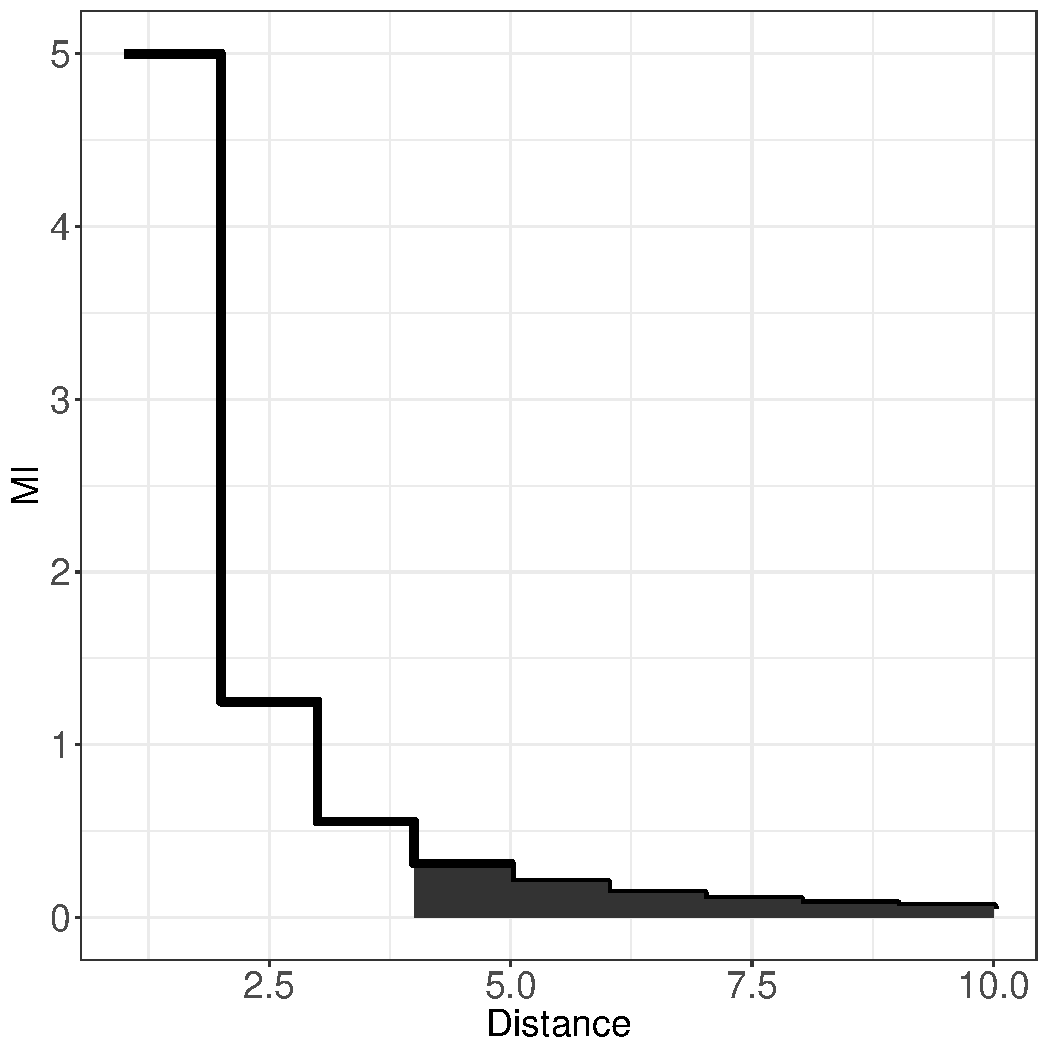
\includegraphics[width=0.45\textwidth]{../code/toy/figures/add-surp.pdf}
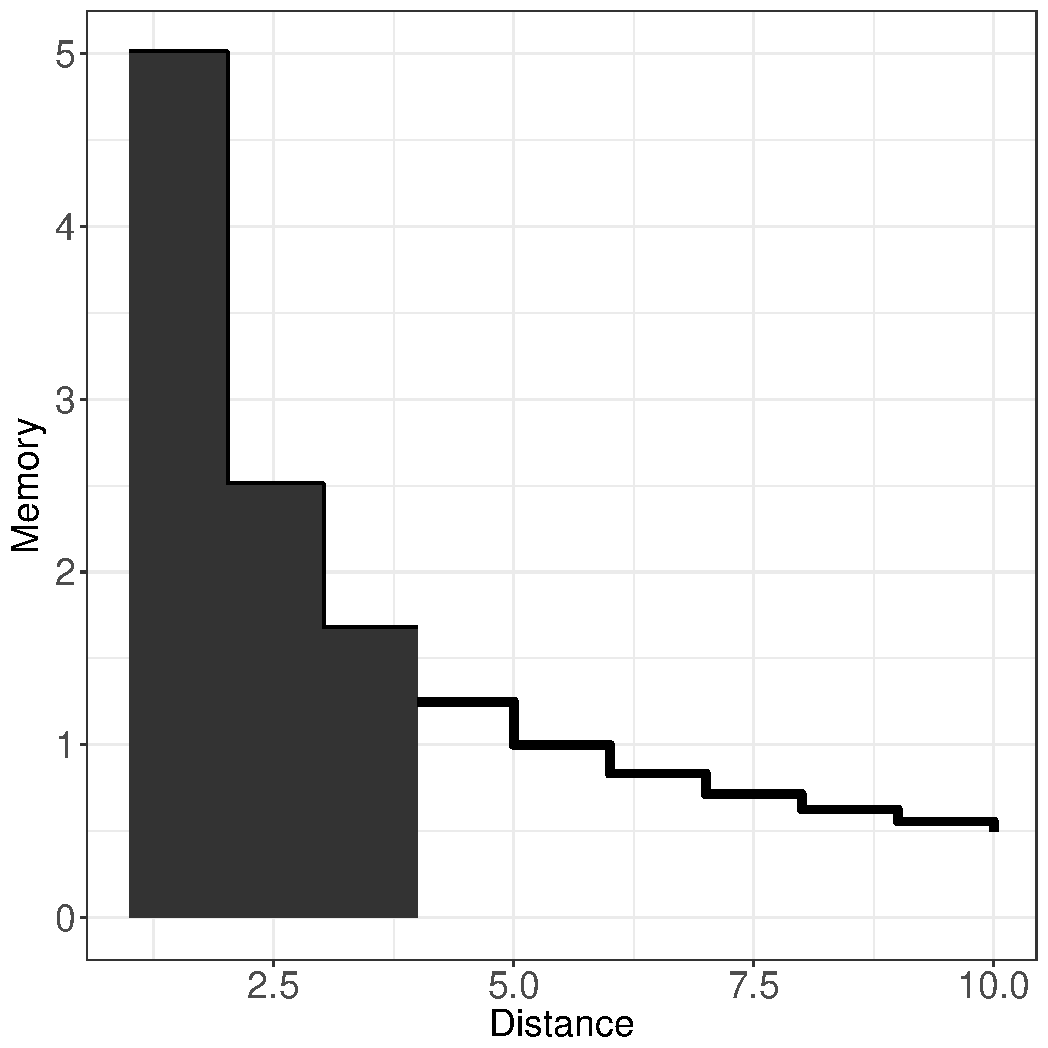
\includegraphics[width=0.45\textwidth]{../code/toy/figures/lower-mem.pdf}
	\caption{Illustration for Proposition~\ref{prop:suboptimal}. Listeners can trade off memory and surprisal: A listener only investing memory of the amount given by the black area on the right will incur at least the black area on the left in additional surprisal. In the given example, $T=4$. By varying $T$, the two areas describe the listener's memory-surprisal tradeoff curve.}\label{fig:listener-tradeoff-decay}
\end{figure}




\begin{figure}
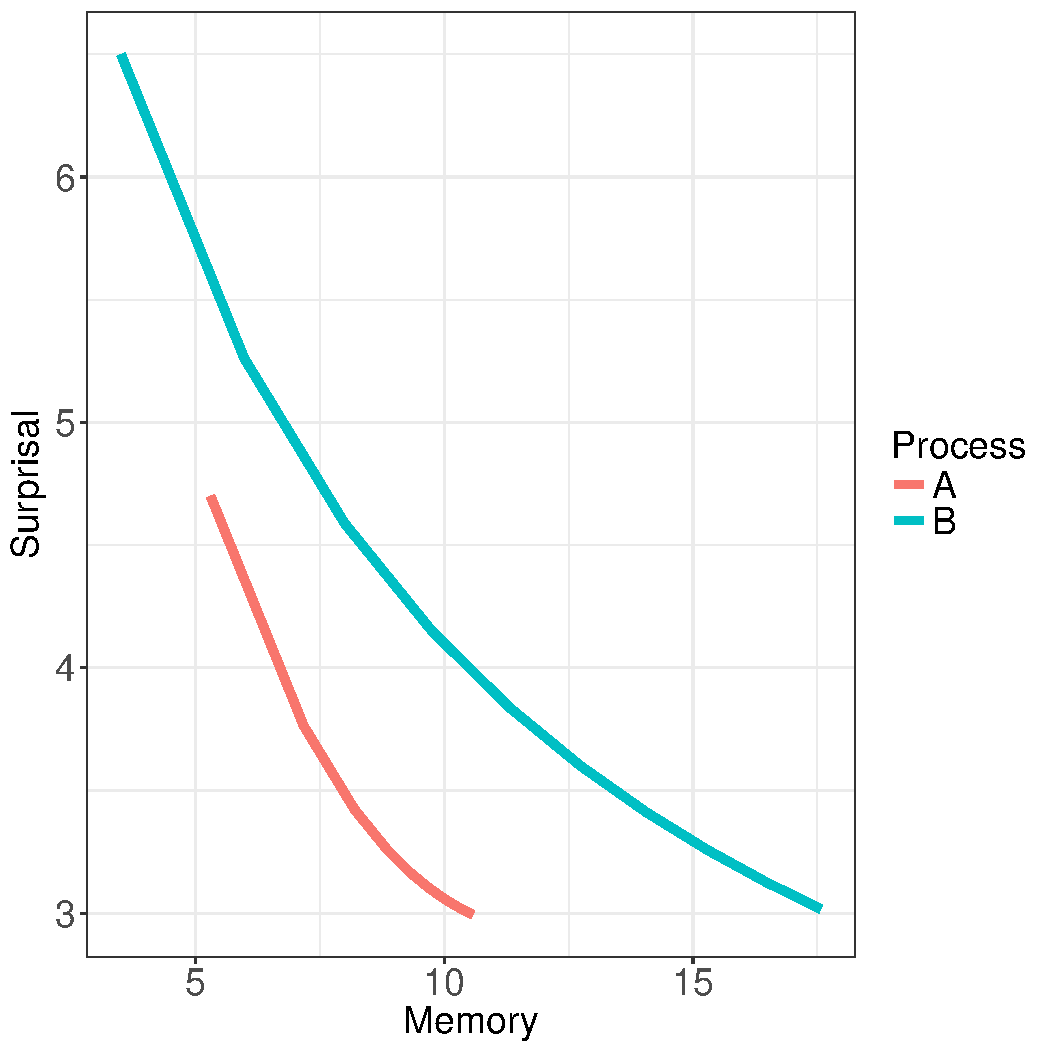
\includegraphics[width=0.45\textwidth]{../code/toy/figures/listener-tradeoff.pdf}
	\caption{Listener's memory-surprisal tradeoff for the two processes in Figure~\ref{fig:basic}. Recall that the red process had a faster decay of conditional mutual information. Correspondingly, this figure shows that a listener can achieve lower surprisal at the same level of memory load.}\label{fig:listener-tradeoff}
\end{figure}




%\subsection{Formal Analysis and Proofs}













\section{Information Locality}\label{sec:info-locality}
\mhahn{not sure about this section}
TODO derive information locality

Due to the factor $t$ inside each term of the sum, carrying the same amount of information over longer distances requires more memory -- that is, modeling long statistical dependencies is more costly in terms of memory than modeling shorter ones.
This formalizes a general, assumption-free, link between memory and locality in language production.
In Section~\ref{sec:listener}, we will extend this analysis to listeners performing incremental prediction.
%incremental prediction.

%We will write $I_t$ as an abbreviation for $\operatorname{I}[w_t, w_0 | w_1, ..., w_{t-1}]$.
The proposition implies that memory is decreased if $I_t$ decreases quickly as $t \rightarrow \infty$ -- that is, if the contributions of long-term dependencies in the process are small.
In particular, memory load can only be finite if $I_t$ decreases fast enough for the infinite sum to converge to a finite value.
%This confirms the intuition that finiteness of memory entails that the contribution of long-term 

%\paragraph{Discussion}
%We have treated the process $(w_t)_t$ as a discrete-time process whose time steps correspond to words, but this is immaterial to the analysis.
%The analysis is not even restricted to discrete timesteps: We can replace thes sum in Proposition~\ref{prop:suboptimal} with an integral to get a continuous-time version.

We illustrate Proposition~\ref{prop:lower-bound} in Figure~\ref{fig:basic}.
We consider two processes A and B, where $I_t := 5t^{-1.5}$ for $A$ and $I_t := 3.5 t^{-2.5}$ for $B$.
The curves of $I_t$, as a function of the distance $t$, are shown in Figure~\ref{fig:basic} (left).
In both cases, $I_t$ converges to zero as $t$ grows to infinity. 
However, $I_t$ decays more quickly for Process A (red).
This means that predictive information about an observation is concentrated more strongly in the recent past.
In Figure~\ref{fig:basic} (right), we show $t\cdot I_t$ as a function of $t$.
Note that the area under the curve is equal to (\ref{eq:memory-bound}).
This area is smaller for the red process, as $I_t$ decays more quickly there.  


\section{Experiment 1: Memory and Dependency Length}




We illustrate the linguistic predictions of Proposition \ref{prop:lower-bound} by reanalyzing the data from \cite{fedzechkina-human-2017}.
This is a miniature artificial language study that showed a bias for Dependency Length Minimization in production in artificial language learning.
Due to the controlled setting, it is possible to exactly compute the speaker's memory as given in~(\ref{eq:memory-bound}).


As ~(\ref{eq:memory-bound}) is invariant under reversal of the language, we only consider the head-final version of her artificial language.
The language has consistent head-final order, and uses case marking on objects.
The relevant production targets are transitive sentences where one of the two arguments is much longer than the other, due to the presence of a PP modifier, as shown in Table~\ref{tab:artificial}.
The language has variable order of subjects and objects; for the production targets, the B versions produce much longer dependencies than the A versions.
Dependency Length Minimization thus predicts that speakers are more likely to use the A versions.
\cite{fedzechkina-human-2017} confirmed this experimentally.


\begin{table}
	\textbf{A Orders: Short Dependencies}

		\begin{tabular}{ccc}
			Object & Subject & Verb \\
			\fbox{\begin{tabular}{llllll}
				\fbox{\begin{tabular}{llll} Adjective &Noun &Postposition\end{tabular}} & Noun-Case
					\end{tabular}} & \fbox{\begin{tabular}{l}Noun\end{tabular}} & \fbox{\begin{tabular}{l}Verb\end{tabular}}  \\
		\end{tabular}
\\
		\begin{tabular}{ccc}
			Subject & Object & Verb \\
			\fbox{\begin{tabular}{llllll}
				\fbox{\begin{tabular}{llll} Adjective &Noun &Postposition\end{tabular}} & Noun
					\end{tabular}} & \fbox{\begin{tabular}{l}Noun-Case\end{tabular}} & Verb \\
		\end{tabular}
\\
\\

	\textbf{B Orders: Long Dependencies}


		\begin{tabular}{ccc}
			Subject & Object & Verb \\
			 \fbox{\begin{tabular}{l}Noun\end{tabular}} &  \fbox{\begin{tabular}{llllll}
				\fbox{\begin{tabular}{llll} Adjective &Noun &Postposition\end{tabular}} & Noun-Case
		\end{tabular}}  &  \fbox{\begin{tabular}{l}Verb\end{tabular}}  \\
		\end{tabular}
\\
		\begin{tabular}{ccc}
			Object & Subject & Verb \\
			\fbox{\begin{tabular}{l}Noun-Case\end{tabular}} & \fbox{\begin{tabular}{llllll}
				\fbox{\begin{tabular}{llll} Adjective &Noun &Postposition\end{tabular}} & Noun
		\end{tabular}} & Verb \\
		\end{tabular}

			\caption{Production targets in the artificial mini language from \cite{fedzechkina-human-2017}. The language has head-final order, with free variation between SO and OS orders. When one of the arguments is much longer than the other, placing the longer one first (`A' orders) shortens syntactic dependencies, compared to `B' orders.}\label{tab:artificial}

\end{table}

In this section, we show that our bound on speaker memory makes the same prediction, without reference to syntactic structure or specific memory architectures. 

We constructed one language consisting of the A versions, and one language consisting of the B versions.
Following the experimental setup of \cite{fedzechkina-human-2017}, we assigned equal probability to the two possible configurations per language, and used a separate set of nouns (inanimate nouns) for the embedded noun in the long phrase.

We interpreted each of the two languages as a stationary processes, extending infinitely in both directions, by concatenating independent samples drawn from the language.
			We computed (\ref{eq:memory-bound}) from a chain of 1000 independently sampled sentences, for each of the two versions of the toy language.
			Figure~\ref{fig:toy-mis} (left) shows the curve of the conditional mutual information $I_t$ as a function of the distance $t$.
			The curves differ at $t=2$ and $t=5$: 
			About 0.073 nats of predictive information that are at distance $t=2$ in the A orders are moved to $t=5$ in the B orders.
%			In this sense, A orders have greater information locality than the B orders.
			%What is responsible for this difference?
			The source of the difference lies in predicting the presence and absence of a case marker on the second argument -- i.e., whether to anticipate a subject or object.
			In the A orders, considering the last two words is sufficient to make this decision.
			In the B orders, it is necessary to consider the word before the long second constituent, which is five words in the past.

			The total amounts of predictive information -- corresponding to the area under the curve -- are the same, indicating that both languages are equally predictable.
			However, we will see that the memory demands are different:
			Figure~\ref{fig:toy-mis} (right) shows $t\cdot I_t$ as a function of $t$.
			As $I_t$ decays faster in A orders, the total area under the curve now differs between A and B, and is larger in B.
			%This area corresponds to the lower bound in (\ref{eq:memory-bound}), and is 2.21 nats in A orders, and 2.43 nats in B orders.

%While (\ref{eq:memory-bound}) is a general lower bound, it can be proven that this bound is actually tight in the case of this specific example.\footnote{This can be shown by computing the causal states and then showing that the crypticity is zero, both of which is tractable in the case of this small-scale artificial language.}
%That is, a speaker who optimally allocates memory resources will spend 2.21 nats in A orders, and 2.43 nats in B orders.


In Figure~\ref{fig:toy-listener-tradeoff}, we show the resulting curve for the two versions of the artificial language from \cite{fedzechkina-human-2017}.
%In this language, speaker memory coincides with the memory demand of a listener who performs optimally in incremental prediction.
The curve shows that, at any desired level of surprisal, Order A requires at most as much memory as Order B.
For reaching optimal surprisal, Order A requires strictly less memory.
Thus, in this case, the listener's surprisal-memory tradeoff is optimized by the orders predicted by Dependency Length Minimization.

It is important to stress that, even though we computed this value by considering the number of words impacting predictions at a given point in time, this bound holds independently of the actual implementation and architecture of memory and predictions.




\begin{figure*}
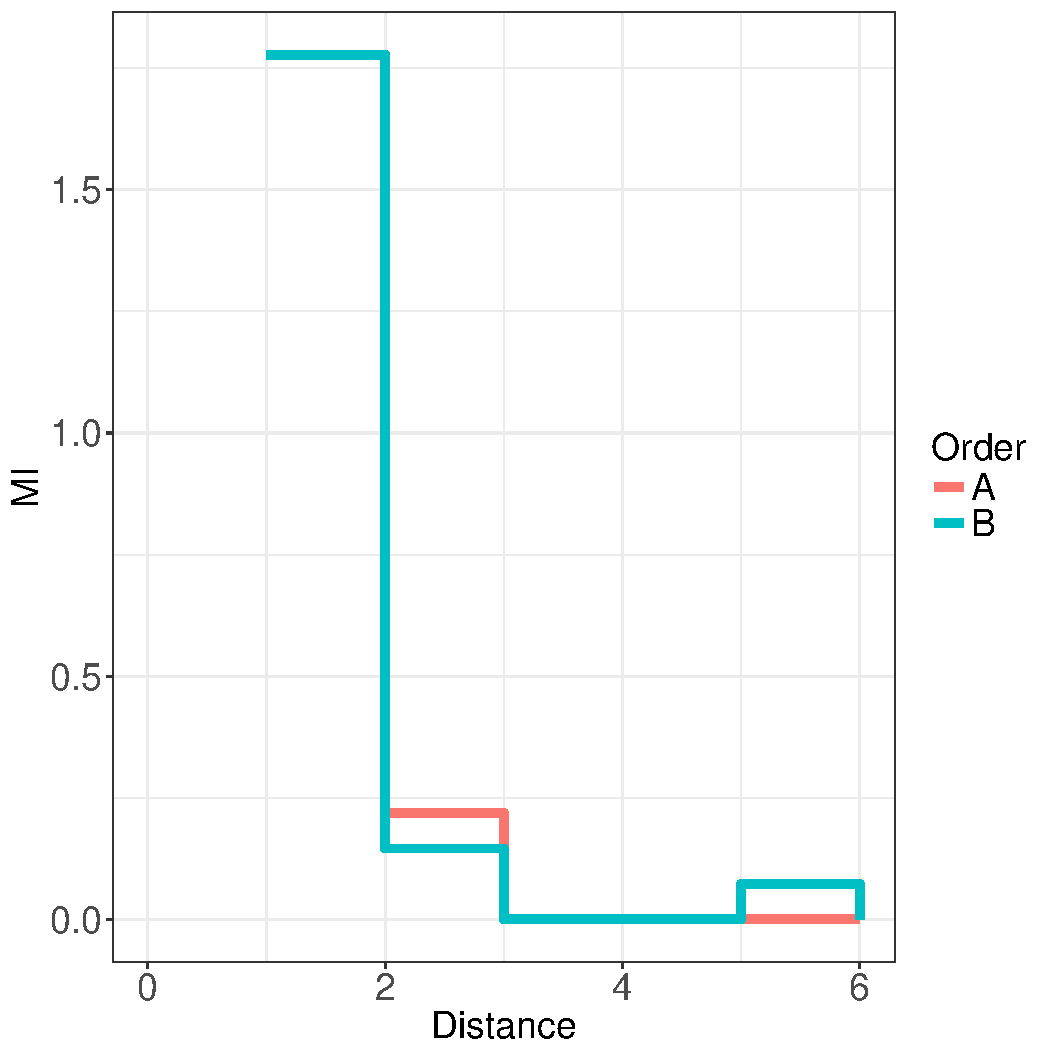
\includegraphics[width=0.45\textwidth]{toy/toy-mis.pdf}
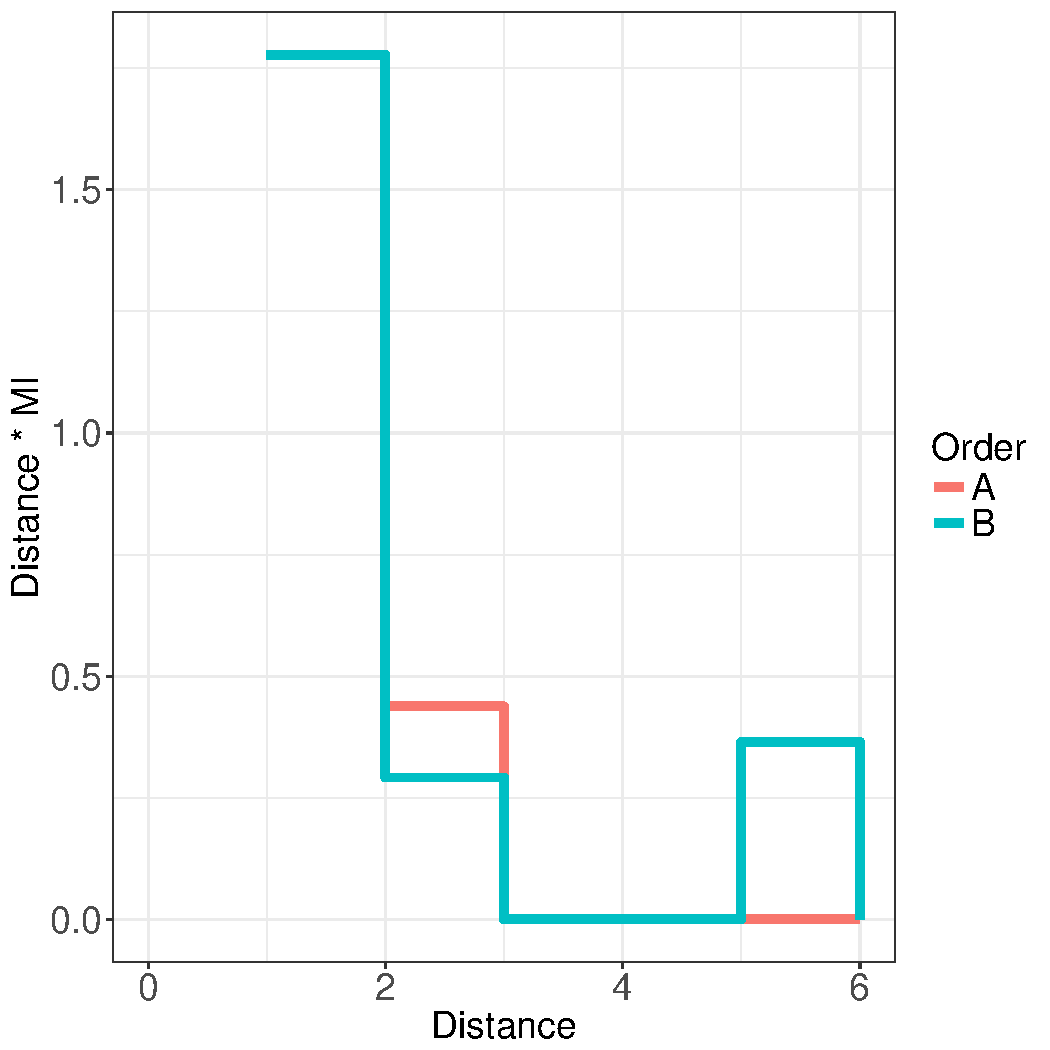
\includegraphics[width=0.45\textwidth]{toy/toy-t-mis.pdf}
%
	\caption{Left: Decay of Conditional Mutual Information, as a function of the distance $t$, for the two versions in the artificial language. The areas under the two curves are identical, corresponding to the fact that both orders are equally predictable. However, mutual Information decays faster in Order A.\ \ \ Right: $t I_t$, as a function of $t$. The area under the B curve is larger, corresponding to larger memory demand for this order.}\label{fig:toy-mis}
\end{figure*}
%Both languages have the same overall entropy rate, but they differ in the distribution of predictive information.
%
%plot of $I_t$
%
%The areas under the curves are identical.
%
%good version
%
%%CONTEXT LENGTH 0   2.06856758681  9997.93143241   0.0
%%CONTEXT LENGTH 1   0.29195106479  1.77661652202   1.77661652202
%%CONTEXT LENGTH 2   0.0729865489103  0.21896451588   2.21454555377
%%CONTEXT LENGTH 3   0.0729865489103  0.0   2.21454555377
%%CONTEXT LENGTH 4   0.0729865489103  0.0   2.21454555377
%%CONTEXT LENGTH 5   0.0729865489103  0.0   2.21454555377
%%CONTEXT LENGTH 6   0.0729865489103  0.0   2.21454555377
%
%bad version
%
%%CONTEXT LENGTH 0   2.06937301571  9997.93062698   0.0
%%CONTEXT LENGTH 1   0.291673373027  1.77769964269   1.77769964269
%%CONTEXT LENGTH 2   0.145830550934  0.145842822093   2.06938528687
%%CONTEXT LENGTH 3   0.145830550934  0.0   2.06938528687
%%CONTEXT LENGTH 4   0.145830550934  0.0   2.06938528687
%%CONTEXT LENGTH 5   0.0729152754672  0.0729152754672   2.43396166421
%%CONTEXT LENGTH 6   0.0729152754672  0.0   2.43396166421
%%CONTEXT LENGTH 7   0.0729152754672  0.0   2.43396166421
%%
%
%
%
%%
%%grammar:
%%
%%S $\rightarrow$ Obj Subj V (1/2) | Subj Obj V (1/2)
%%
%%Obj $\rightarrow$ NP di
%%
%%Subj $\rightarrow$ NP
%%
%%NP $\rightarrow$ N (3/4) | PP NP (1/8) | Adj NP (1/8)
%%
%%PP $\rightarrow$ NP P
%%
%
%

\begin{figure}
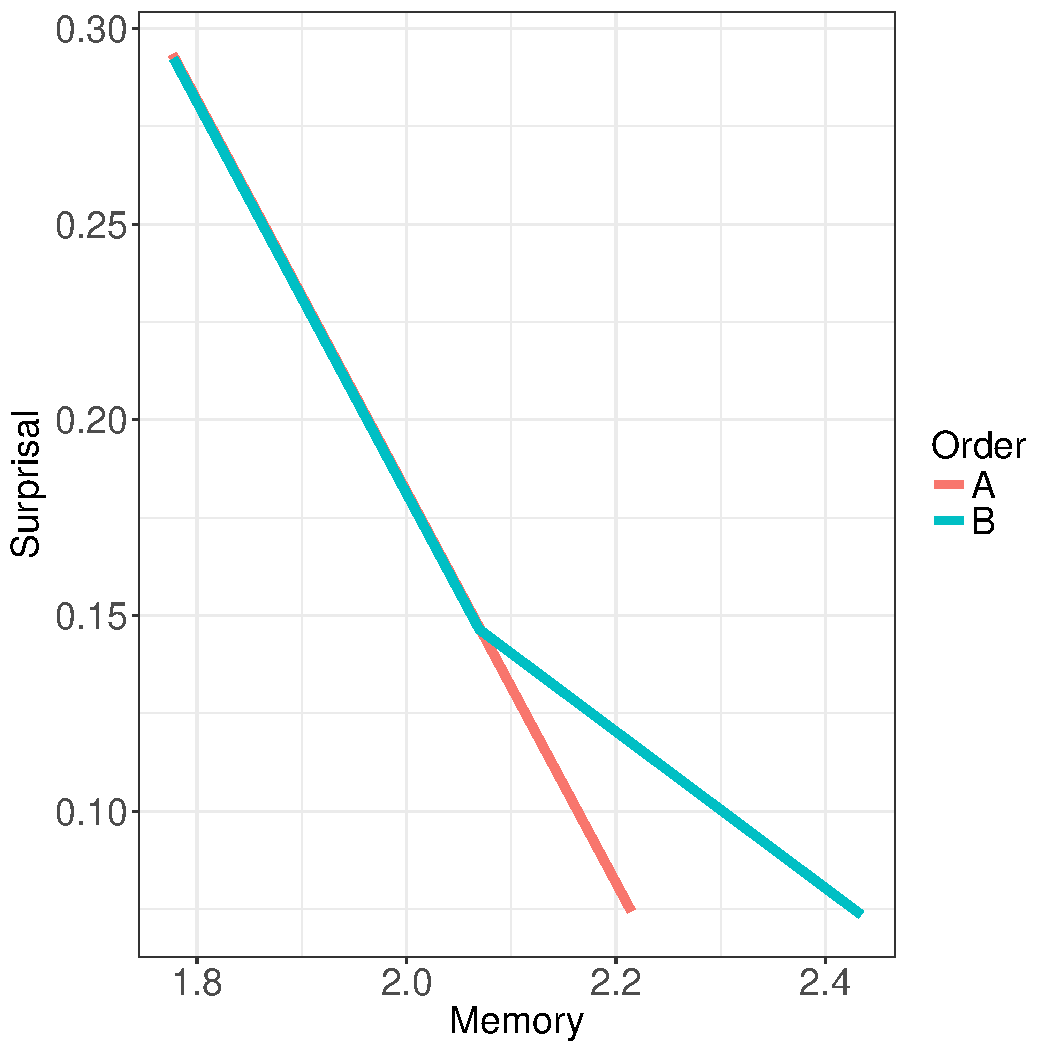
\includegraphics[width=0.45\textwidth]{toy/toy-mem-surp.pdf}
	\caption{Tradeoff between listener memory and surprisal, for the two versions of the artificial language from \cite{fedzechkina-human-2017}. Language A requires less memory at the same level of surprisal.}\label{fig:toy-listener-tradeoff}
\end{figure}





\section{Large-Scale Evidence that natural language optimize Memory-Surprisal Tradeoff}



We now investigate whether word orders as found in natural language reflect optimizization for the memory-surprisal tradeoff.
We compare the memory-surprisal tradeoffs of 52 actual languages to those of counterfactual reorderings.
We compare to counterfactual reorderings that differ from the actual languages in their word order rules, i.e., the rules that determine how syntactic structures are ordered into strings of words.\mhahn{where introduce the idea of word order}.
To create such counterfactual reorderings, we parameterize these word order rules using a method introduced by Gildea and colleagues \citep{gildea-optimizing-2007, gildea-grammars-2010, gildea-human-2015}.

\begin{figure}
\centering
\begin{dependency}[theme = simple]
   \begin{deptext}[column sep=1em]
	   I \&	   wrote \& risāla \& li \& sadīq  \\
   \end{deptext}
	%   \deproot{3}{ROOT}
   \depedge{1}{2}{obj}
	%   \depedge[edge start x offset=-6pt]{2}{5}{ATT}
   \depedge{1}{4}{obl}
   \depedge{4}{3}{case}
   %\depedge[arc angle=50]{7}{6}{ATT}
\end{dependency}
	\caption{TODO Dependencies example}\label{fig:dependency}
\end{figure}


\mhahn{at some point the whole idea of syntactic structures have to be introduced}

\subsection{Data}
We draw on corpora annotated with syntactic structures.
The Universal Dependencies project has compiled such annotated corpora for several dozen languages~\citep{nivre-universal-2017}.
These are annotated in the format of Dependency Grammar.

\paragraph{Dependency Grammar}
In dependency corpora, sentences are annotated with \emph{dependency trees} (Figure~\ref{fig:dependency}).
These are directed trees describing the grammatical relations among words. For example, the arcs labeled ``obj'' represent that the noun in question is the \emph{direct object} if the verb, rather than e.g. the subject or an indirect object.
A dependency arc is drawn from a \emph{head} (e.g. TODO in Figure TODO) to a \emph{dependent} (e.g. TODO).
Dependency trees can be defined in terms of many different syntactic theories \citep{corbett1993heads}.
Although there are some differences in how different formalisms would draw trees for certain sentences, there is broad enough agreement about dependency trees that it has been possible to develop large-scale dependency-annotated corpora of text from dozens of languages \cite{nivre2017universal}.
\mhahn{currently this is taken from the Greenberg paper}

\paragraph{Corpora}
We considered all languages for which there are Universal Dependencies 2.3 treebanks with a total of at least 500 sentences of training data.
We excluded data from historical languages.\footnote{Ancient Greek, Classical Chinese, Coptic, Gothic, Latin, Old Church Slavonic, Old French.}
This resulted in 54 languages.

For each of these languages, we pooled all available corpora in one dataset.
We excluded corpora that primarily contain code-switched text\footnote{Hindi English corpus}, or text created by non-native speakers.\footnote{ESL for English, CFL for Chinese}
Universal Dependencies corpora have a predefined split into \emph{training}, \emph{held-out} (also known as \emph{development}), and \emph{test} partitions.
While larger corpora have all three partitions, smaller corpora often have only some of these partitions.
For most language, we used the predefined data split, separately pooling data from the different partitions. %We did not use the test partitions.
For some languages with little data, there is no predefined training partition, or the training partition is smaller than the other partitions.
In these cases, we redefined the split to obtain more training data:
For these languages, we pooled all the available partitions, used 100 randomly selected sentences as held-out data, and used the remainder as training data.\footnote{This affects Amharic, Armenian, Breton, Buryat, Cantonese, Faroese, Kazakh, Kurmanji, Naija, Thai, and Uyghur.}
For each language, we used the training and held-out sets for estimating the memory-surprisal tradeoff (see Section~\ref{sec:method}).
We provide the sizes of the resulting datasets in Table~\ref{tab:corpora}.



\subsection{Baselines: Counterfactual Ordering Grammars}
We define ordering grammars, small models of the rules by which languages order syntactic structures into sentences.
Our formalism of ordering grammars adapts the method of \cite{gildea-optimizing-2007, gildea-grammars-2010, gildea-human-2015} to the setting of dependency corpora.

Universal Dependencies defines 37 universal syntactic relations that are used to label dependency arcs across all corpora.
These relations encode cross-linguistically meaningful relations such as subjects, objects, and adjectival modifiers.
We define ordering grammars by assigning a parameter $a_\tau \in [-1,1]$ to every one of these 37 universal syntactic relations.
Relations sometimes have language-specific subtypes; we do not distinguish these subtypes.\mhahn{give an example to make clear what this refers to}

Following Gildea and colleagues, this parameter defines how dependents are ordered relative to their head:
Given a head and a set of dependents, we order each dependents by the parameter $a_\tau$ assigned to the syntactic relation linking it to the head.
Dependents with negative weights are placed to the left of the head; dependents with positive weights are placed to the right.

Ordering grammars describe languages that have consistent word order:
For instance, the subject is consistently ordered before or after the verb, depending on whether the parameter for the verb-subject dependency is positive or negative.

We define baseline grammars by randomly sampling the parameters $a_\tau$.
Such baseline grammars define languages that have consistent word order, but do not exhibit any systematic correlations between the orderings of different dependents.



\paragraph{Discussion}
In actual languages, the ordering of words is largely determined by the syntactic relations (CITE).
However, certain kinds of rules cannot be modeled by our word order grammars, such as rules sensitive to the category of the dependent (e.g., differences between nominal and pronominal objects).
Word order freedom also is not modeled.
In this sense, ordering grammars represent approximations to the kinds of ordering rules found in natural language \cite{gildea-optimizing-2007, gildea-grammars-2010, gildea-human-2015}.



\subsection{Estimating Memory-Surprisal Tradeoff}\label{sec:method}
To estimate mutual informations, we use LSTM recurrent neural networks, the basis of the state of the art in modeling natural language (CITE)\footnote{We note that the state-of-the-art is now achieved by other models when extremely large amounts of training data (on the order of several dozen GB of texts) are available. In comparison, LSTMs remain state of the art on small/medium training data such as the UD corpora.} and predicting the surprisal effect on reading times~\citep{frank-insensitivity-2011, goodkind-predictive-2018}.
We provide data from alternative estimation methods in the SI.



\paragraph{Model and Parameter Estimation}
We use a recurrent neural network with Long-Short-Term Memory cells~\citep{hochreiter-long-1997} (CITE for Neural LM).
This architecture takes as input a sequence $x_1 ... x_N$ of words, and at each time step $t=1, ..., N$, calculates a probability distribution $p(w_t|w_1...w_{t-1})$ over the next word $w_{t}$ given preceding words $w_1 ... w_{t-1}$.
Our model specification follows (CITE someone who used exactly the same model).

The network is parameterized by a vector $\theta$ of weights determining how the activations of neurons propagate through the network~\citep{hochreiter-long-1997}.
Given a corpus, the numeral parameters of the LSTM are chosen so as to minimize the average surprisal across the training corpus.
%We can think of the LSTM parameters as forming one large vector $\theta$.
At the beginning of training, the parameters $\theta$ are randomly initialized to some setting $\theta_0$.

The training corpus is chopped into word sequences $w_1 ... w_{T_{max}}$ of length ${T_{max}}$, where ${T_{max}}$ is the highest $T$ for which we estimate $I_T$. %  (${T_{max}} = 20$ in our experiments).
We use Stochastic Gradient Descent to optimize the parameters $\theta$ so as to minimize the surprisal
\begin{equation}\label{eq:train}
	\frac{1}{T_{max}} \sum_{i=1}^{T_{max}} \log p_\theta(w_i|w_1...w_{i-1})
\end{equation}
When calculating the parameter update, we use three standard methods of regularization that have been shown to improve neural language modeling: dropout~\citep{srivastava-dropout:-2014}, word dropout, and word noising~\citep{xie2017data}.

Once all sequences have been processed, we start another pass through the training data.
Before each pass through the training data, the order of sentences of the training data is shuffled, and the corpus is again chopped into sequences of length $T$.
After each pass through the training data, the average surprisal~(\ref{eq:train}) at the current parameter setting $\theta$ is evaluated on the held-out partition.
We terminate training once this held-out  surprisal does not improve over the one computed after the previous pass any more.

In our experiments, we chose $T_{max} = 20$. Prior work has found that the probabilities $p(w_t|w_1...w_{t-1})$ are dominated by a small number of preceding words \citep{daniluk2017frustratingly}, suggesting that $I_t$ will be close to zero for $t$ greater than 20.



\paragraph{Choice of Hyperparameters}

The LSTM model has a set of numerical \emph{hyperparameters} that need to be specified before parameter estimation, such as the number of recurrent neurons and the learning rate. %namely the dimensionalities of the embeddings $d_{emb}$, the dimensionality of the hidden states $d_{LSTM}$, and the number of LSTM layers $d_{layer}$, the learning rate $\alpha$, and the regularization parameters (dropout rate $p_{embedding}$, word dropout rate $p_{word}$, word noising rate $p_{noising}$).
For each corpus, we used Bayesian optimization using the Expected Improvement acquisition function \citep{snoek-practical-2012} to find a good setting of the hyperparameters.
We optimized the hyperparameters to minimize average surprisal~(\ref{eq:train}) on the held-out partition resulting at the end of parameter estimation, on languages generated from random word order grammars.
This biases the hyperparameters towards modeling counterfactual grammars better, biasing them \emph{against} our hypothesis that real orders result in better memory-surprisal tradeoffs than counterfactual orders.

Due to reasons of computational efficiency, neural language models can only process a bounded number of distinct words in a single language (CITE).
For each corpus, we limited the number of distinct processed words to the $N=10,000$ most common words in the training corpus, a common choice for neural language models (CITE).
Following (CITE), we represented other words by their part-of-speech tags as annotated in the corpora.
This applied to 37 languages, affecting an average of 11~\% of words in these languages.
We believe that this modeling limitation does not affect our results for the following reasons.
First, this affects the same words in real and counterfactually ordered sentences.
Second, all excluded words are extremely infrequent in the available data, occurring less than 10 times (except for Czech and Russian, the languages for which we have by far the largest datasets).
Many of the excluded words occur only once in the dataset (78 \% on average across the affected languages).
This means that any model would only be able to extract very limited information about these words from the available training data, likely \emph{less} than what is provided by the part-of-speech tag.
Third, traditional N-gram models, which do not have this limitation, provide results in qualitative agreement with the neural network-based estimates (see SI).




\paragraph{Estimating the Memory-Surprisal Tradeoff Curve}



The quantity $I_t$ in~(\ref{eq:memory-bound}) is equal to the difference 
\begin{equation}
\operatorname{I}[w_t, w_0 | w_1, ..., w_{t-1}] = H[w_t|w_1, ..., w_{t-1}] - H[w_t|w_0, w_1, ..., w_{t-1}]
\end{equation}
This quantity can be estimated as follows.
After estimating the parameter vector $\theta$, we compute the following difference for each word $w_t$ ($t$ ranging from $T_{max}$ up to the length of the held-out partition) in the held-out partition:
\begin{equation}
	\frac{1}{|HeldOut|-t} \sum_{i=t}^{|HeldOut|} \log P_\theta[w_i | w_{i-t}, w_{i-t+1}, ..., w_{i-1}] - P_\theta[w_i | w_{i-t+1}, ..., w_{i-1}]
\end{equation}
and take the average over these.
We cut $T$ off at 20, as this is the length of the sequences processed by the model.

%We then used linear interpolation to interpolate the surprisal value for memory values in between these values. (TODO make a figure).\mhahn{mention linear interpolation already when explaining how to get tradeoff from theorem}
%This is justified theoretically (TODO maybe discuss when introducing the theorem).

We estimate the unigram entropy $H[w_0]$ by averaging over all models.

For each language, we collected data from the actual orderings and from several random grammars.
We collect multiple samples for the actual orderings to control for variation due to the random initialization of the neural network.
For each of the random grammars, we collect one sample.
Data is collected according to a precision-based stopping criterion described in Section (REF).

\subsection{Statistics}

We now describe how we compared memory-surprisal tradeoffs between real and baseline languages.

%For each sample, we estim
%For each language, we viewed surprisal as a function of memory.
%We used linear interpolation to obtain surprisal values for all levels of memory.

We want to test whether languages' surprisal-memory tradeoffs better than those of most baseline languages.
%We view surprisal as a function of memory load, so that the curve is defined on all of $\mathbb{R}_+$.
We compare real and baseline languages by evaluating which languages result in lower surprisal at the same level of memory.
We now describe the statistics we use to quantifying the difference between real and baseline languages.
We do everything in a frequentist framework (null hypothesis testing \& confidence intervals), as we can do exact tests and confidence intervals without parametric assumptions.
\mhahn{Maybe we can explain how the tests \& CIs also have reasonable Bayesian interpretations (for the specific methods used here, rejection of the null should guarantee that the posterior of the null hypothesis is small under a wide range of priors.).}

\paragraph{Median Surprisal and Confidence Interval for Medians}
We compute surprisal at 40 evenly spaced points of memory (selected individually for each language), over all runs for the real language, and over all baselines grammars.
We then compute the median surprisal over all runs for the real language, and over all baselines grammars.
We compute a confidence interval for this median surprisal, using the binomial PDF. \mhahn{some standard stats reference}
This interval is exact, without parametric assumptions or asymptotic approximations.

% yStudyTradeoff_Bootstrap_Parallel_OnlyWordForms_BoundedVocab_BinomialTest_Single_MedianCI.py


%\paragraph{CI for Median Difference}
%We create (nonparametric and nonasymptotic) confidence interval for the difference between real and baseline median surprisals at each memory value.
%\mhahn{the resulting plots are not very intuitive, might scrap this}
%
%% yStudyTradeoff_Bootstrap_Parallel_OnlyWordForms_BoundedVocab_BinomialTest_Single_MedianDiffCI.py


\paragraph{Pointwise Significance Test}
At five evenly spaced memory values $\mu$ (chosen per language), we do a nonparametric and nonasymptotic significance hypothesis test against the null hypothesis that at least half of the baseline grammars have lower surprisal than the actual language (Figure~\ref{fig:nhst-pointwise}).
Formally, let $W_-(\mu)$ be the proportion of baseline languages that have strictly lower surprisal than the real language at memory level $\mu$.
For each level $\mu$ of memory, we consider the null hypothesis that
\begin{equation}
	W_-(\mu) \leq 0.5
\end{equation}
In this test, we approximate the surprisal value of the real language by the \emph{sample median}.
%In reality, we do not observe the curve of the real language exactly, but as noisy samples from our computational estimator.
We use the Binomial Test.

%This statistic also should have a reasonable Bayesian interpretation:
% E.g., if the random samples are unimodal, and we do inference over only the median (location family), 



\begin{figure}
	\begin{center}
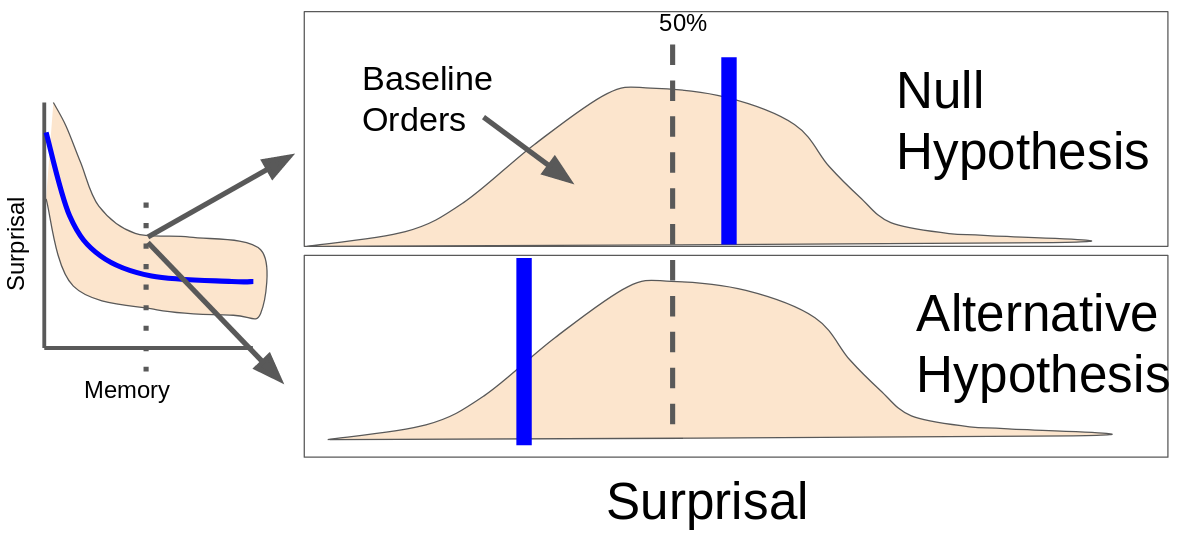
\includegraphics[width=0.45\textwidth]{figures/nhst.png}
\end{center}
	\caption{Illustration for the pointwise null-hypothesis significance test. At a given level of memory, we test against the null hypothesis that at least half of the baseline orders provide lower surprisal than the real language.}\label{fig:nhst-pointwise}
\end{figure}






%For each memory value $\mu$, we do a significance test (nonparametric and nonasymptotic).
%\begin{equation}
%	W_+(\mu) \geq W_-(\mu)
%\end{equation}
%We use the empirical median for the real language.

% yStudyTradeoff_Bootstrap_Parallel_OnlyWordForms_BoundedVocab_BinomialTest_Single.py

%We take the REAL values to be estimated exactly by their medians.



\paragraph{Pointwise Quantile Estimate}
%CI for quantile: % yStudyTradeoff_Bootstrap_Parallel_OnlyWordForms_BoundedVocab_BinomialTest_Single_UnimodalBoundOnQuantile_BothDirections.py
%\mhahn{might scrap the CI}


\begin{figure}
	\begin{center}
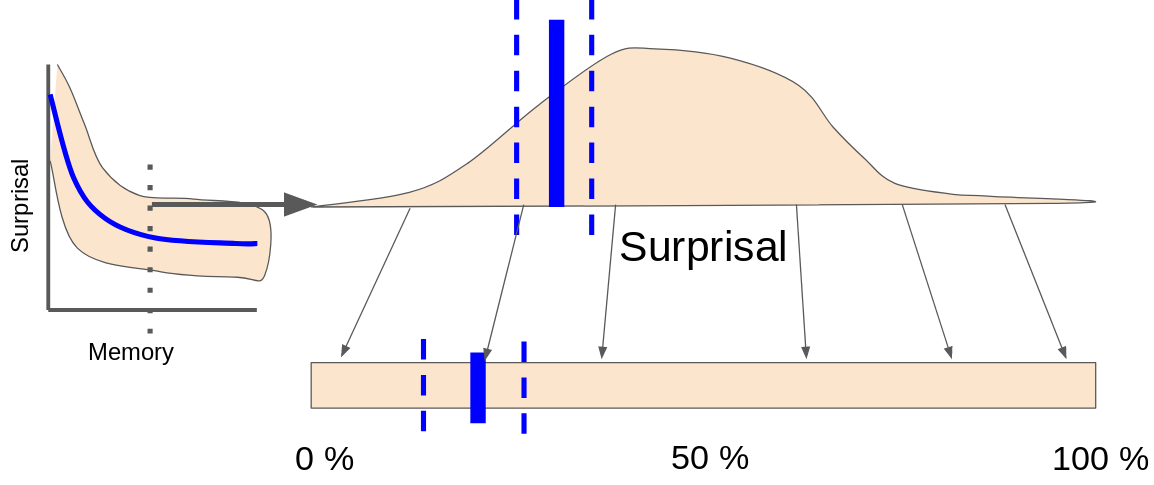
\includegraphics[width=0.45\textwidth]{figures/quantile.png}
\end{center}
	\caption{Illustration for the quantile estimate. At each level of memory, we provide an estimate of the percentage of baseline languages that have lower surprisal than the real language.}\label{fig:quantile-pointwise}
\end{figure}

To provide estimates of the degree of optimization of real orders, we also compute what \emph{fraction} of baseline languages provides better tradeoffs than the real language.
Specifically, for each level of memory $\mu$, we estimate what percentage of baseline languages have lower (or equal) surprisal than the real language.
This is described in Figure~\ref{fig:quantile-pointwise}.
We use the Binomial Test to derive a confidence lower bound for this quantile (CITE).
Again, we take the REAL values to be estimated exactly by their medians.

%We want to create a CI at each Memory value for the quantile.
%
%At a fixed memory value $\mu$, let $n_+$ be the better baseline samples, $n_-$ the worse (or equal) ones.
%
%We want to get a confidence bound $q$ on $P_{X \sim Baseline}(X < x_{real})$.
%Let $p := P(N_+ \leq n_+ | N_+ + N_-; q)$.
%Then output $(0, q)$ as a level $p$ CI for the parameter $P(X < x_{real})$.
%We minimize $q$ subject to $p < 0.05$.
%This CI is exact in the sense that it does not involve asymptotic approximations or parametric assumptions, but it is extremely conservative.
%
%Also the following does not assume unimodality, and ends up getting about the same intervals
%% yStudyTradeoff_Bootstrap_Parallel_OnlyWordForms_BoundedVocab_BinomialTest_Single_UnimodalBoundOnQuantile_BothDirections_NoAssumption.py




\paragraph{Global Quantile Estimate}

To provide a stopping criterion, we additionally need a global measure of the degree of optimization of the real language.

Due to the use of bootstrapping, the confidence intervals are not exact.

\begin{figure}
	\begin{center}
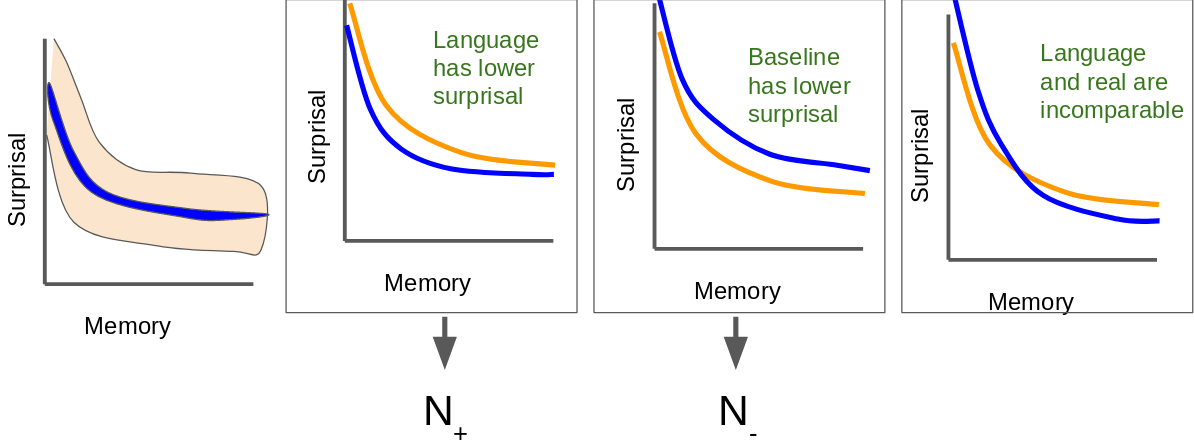
\includegraphics[width=0.45\textwidth]{figures/quantile-global.png}
\end{center}
	\caption{Illustration for the global quantile estimate. For each sample for the real language, we compare the memory-surprisal curve to all baselines.}\label{fig:quantile-global}
\end{figure}



For each sample $x$ from real orderings, we look at the proportions $N_+(x)$ of samples from the baseline languages that are more optimal than $x$ throughout the entire range where both curves are defined, and the proportion $N_-(x)$ of baseline samples that are consistently less optimal.

%We consider the null hypothesis that, on average, not more baseline languages are consistently less optimal than are consistently more optimal than the real orderings:
%\begin{equation}
%	\E_{x \sim P_1}[W_+(x)] \geq \E_{x \sim P_1}[W_-(x)]
%\end{equation}

We estimate the quotient
\begin{equation}\label{eq:g}
	G :=	\frac{\E_{x \sim P_1}[W_+(x)]}{\E_{x \sim P_1}[W_+(x) + W_-(x)]}
\end{equation}
where $P_1$ is the distribution over values obtained for real orderings.
We use a bootstrapped confidence interval for $\E[G]$ for quantifying the degree of optimization.
For bootstrapping, we separately resample samples from the real language and from the baseline grammars.



%- bootstrapping
%- subsampling
%- permutation test / rank test ??
%



\subsection{Number of Samples}
Training neural language models is computationally costly.
Therefore, we used a precision-based stopping criterion to adaptively choose a sample size for each language.
Precision-based stopping criteria offer a way to adaptively choose sample size without biasing results (CITE).

For each language, we first collected 10 data points for real orderings and 10 data points for baseline orderings.
We continued obtaining new data points until the CI for $G$ had width $\leq 0.15$, or there were 100 samples from $P_1$ and 300 samples from $P_2$.
Up to the end, we chose the next sample to be from $P_0$ with probability 2/3, and $P_1$ otherwise.\footnote{Due to a scripting error, a much higher number of samples was generated for Erzya.}

This procedure was parallelized on several machines.
In the case where the stopping criterion was reached for a language while several machines were still computing samples for this language, we did not discard those samples.
Consequently, more samples were collected than necessary to reach the stopping criterion; however, in a way that does not bias our results towards or against our hypothesis.

%Due to parallelization of this procedure, it often produced more samples than required, when the stopping criterion .
%We chose these thresholds based on preliminary simulations which had suggested that these widths were achievable at acceptable computational cost.
%For each language, we collected at least 5 data points for real orderings and at least 10 data points for baseline orderings.
%We continued obtaining new data points until the CI for $G$ had width $\leq 0.15$, or there were 100 samples from $P_1$ and 300 samples from $P_2$.
%Up to the end, we chose the next sample to be from $P_0$ with probability 2/3, and $P_1$ otherwise.




\subsection{Results}




The numbers of samples taken per language are provided in Table~\ref{tab:samples}.

%In Figure~\ref{tab:plain-results} (TODO), we show the estimated memory-surprisal tradeoff curves for all samples.

In Figure~\ref{tab:medians}, we show the medians for real and baseline languages.

Descriptively, the real language provides better tradeoffs than the median of the baselines across languages, with four exceptions (Latvian, North Sami, Polish, Slovak).

In Figure~\ref{tab:slice-hists-real}, we show the distribution of surprisals achieved at the maximal memory value for real and random languages.

In Figure~\ref{fig:hist-real}, we show surprisals at maximum memory, after z-transforming for each individual language and then aggregating.

In Table \ref{tab:median_diffs}, we show the differences in median surprisal, as a function of memory.


In Table~\ref{tab:boot-g}, we report the bootstrap estimates and confidence intervals for G~(\ref{eq:g}).
$\E[G]$ was not estimated to be significantly above $>5$ for four languages: Latvian, North Sami, Polish, and Slovak.


In Table~\ref{tab:quantiles}, we show the quantiles.





\subsection{Discussion}

We have found that 48 out of 52 languages provide better memory-surprisal tradeoffs than random baselines with consistent but counterfactual word order rules.

Four languages provide exceptions; these are Latvian (Baltic), North Sami (Uralic), Polish and Slovak (both Slavic).
All four languages have strong word order freedom (CITE).
Freedom of word order plausibly makes sentences less predictable, as the same syntactic structure can receive different surface realizations.
We thus hypothesized that freedom of word order impacts the memory-surprisal tradeoff, and that languages with more strongly fixed word order should display more optimal memory-surprisal tradeoffs.
%We hypothesized that freedom of word order freedom may be responsible for the difference between these languages and the other languages.

To test this hypothesis, we examined the correlation between word order freedom and the surprisal difference between real and baseline orderings.
To quantify word order freedom, we used a corpus-based estimate, the \emph{branching direction entropy}~\citep{futrell-quantifying-2015}.
This is the entropy of the ordering (head-first or dependent-first) of dependencies conditioned on the dependency label and the part-of-speech label of head and dependent.
%\cite{futrell-quantifying-2015} showed that this me
These two quantities are plotted in Figure~\ref{fig:hist-real}.
We found that branching direction entropy was strongly correlated with the surprisal difference between real and baseline orderings (Spearman correlations -0.58, $p = 7.414e-6$).




\begin{figure}
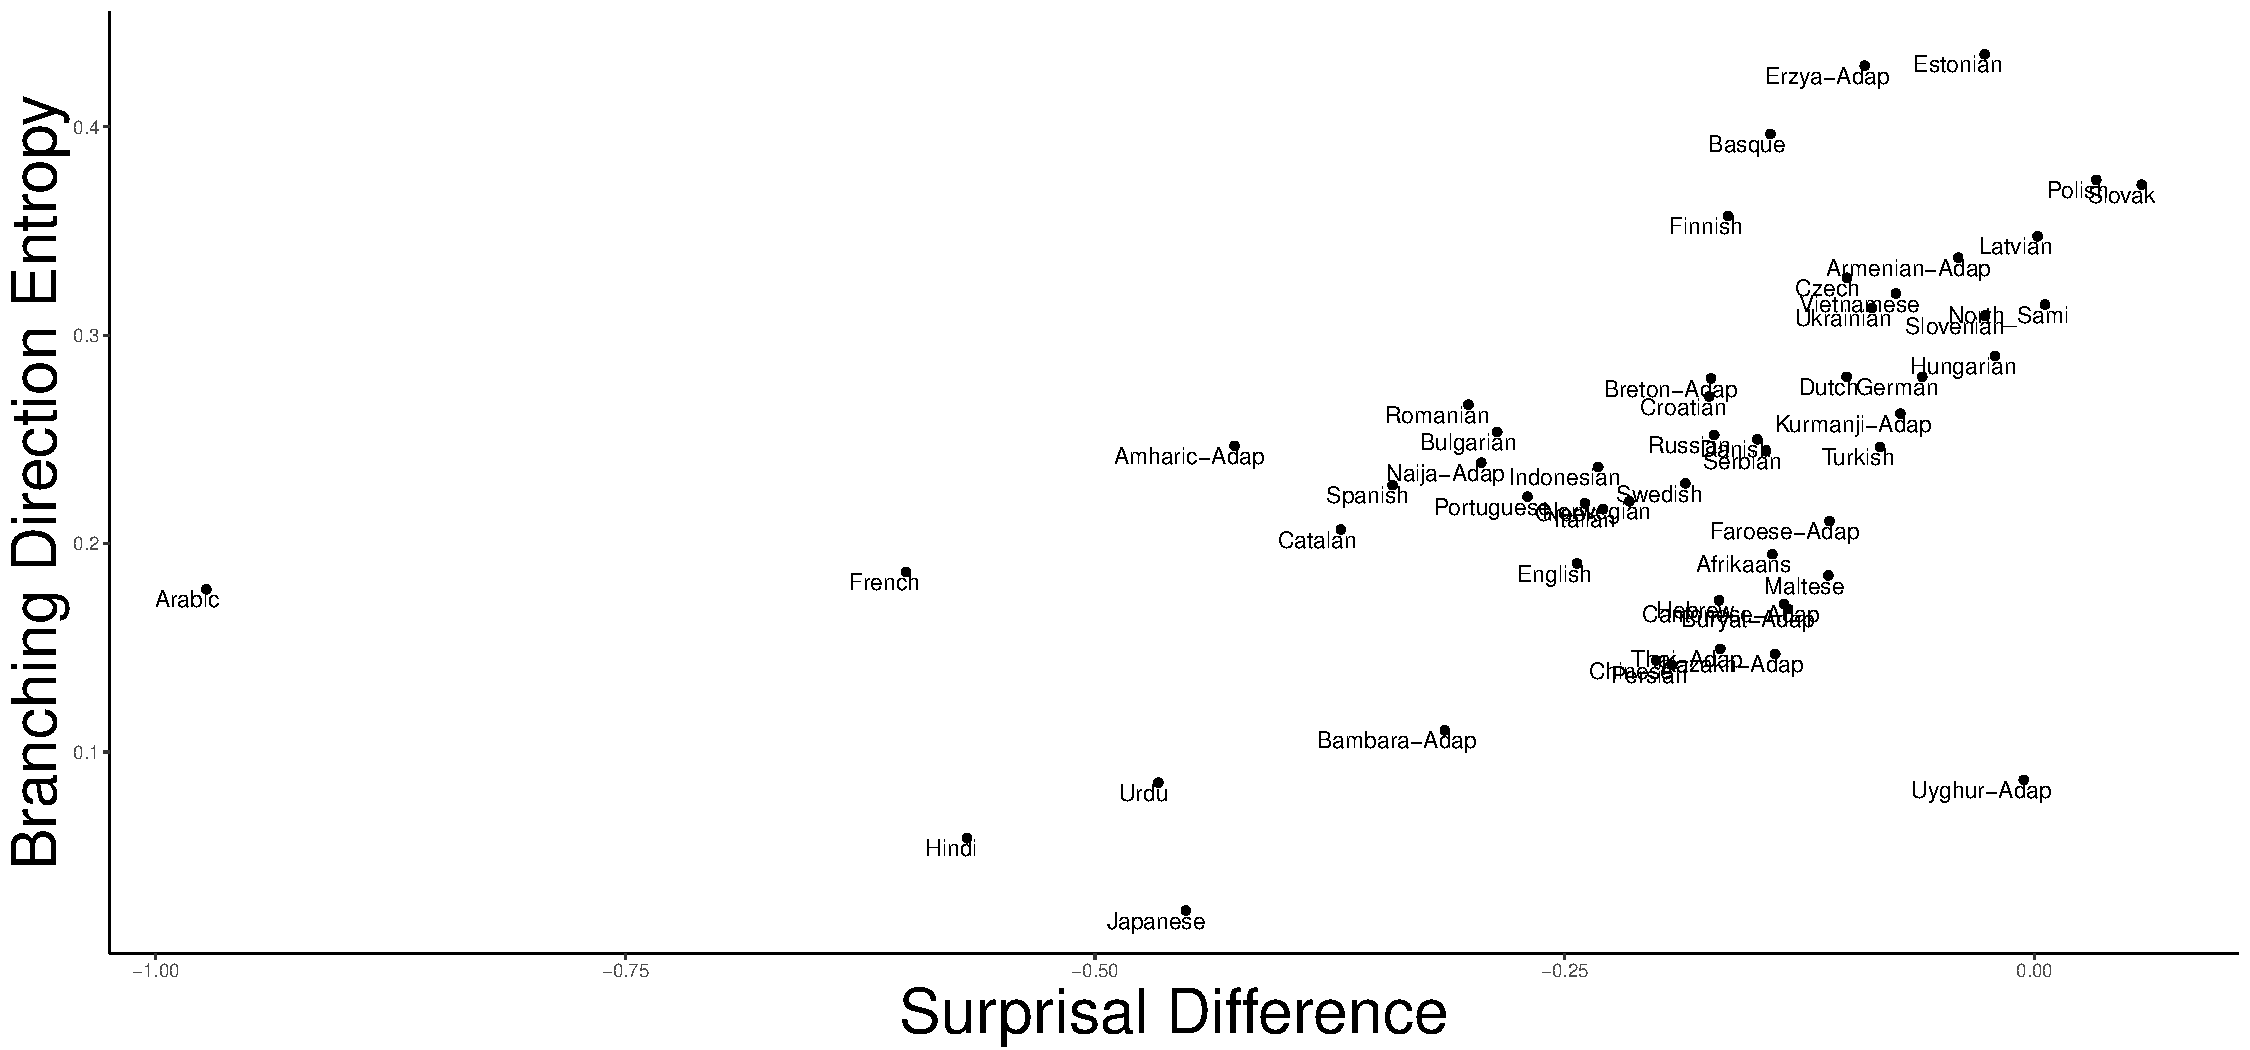
\includegraphics[width=0.95\textwidth]{../code/visualize_neural/figures/surprisal-branching-entropy-REAL.pdf}
	\caption{Surprisal Difference vs Branching Direction Entropy.}\label{fig:hist-real}
\end{figure}


\mhahn{One thing that has to be discussed: the absolute values differ between languages}




\section{Discussion}


\subsection{Other Models of Sentence Processing}

\paragraph{Early Models}

Yngve 1960, had a complexity measure, but doesn't work well for left-branching structures

Miller and Chomsky 1963

Frzier 1985 local nonterminal count

Rambow and Joshi 1994 using TAG

Marcus 1980 deterministic parsing

(Sabrina Gerth, Memory Limitations in Sentence Processing)


\paragraph{Dependency Locality}
The quantity described in Proposition~\ref{prop:lower-bound} is formally similar to Storage Cost in the Dependency Locality Theory (DLT) \citep{gibson-linguistic-1998}: Storage cost at a given timestep is defined as the number of predictions that are held in memory.
Storage cost only considers predictions that are certain, and each prediction takes an equal amount of memory.
In contrast, the result in Proposition~\ref{prop:lower-bound} can be seen as weighting predictions by their certainty and the amount of predictive information.
In this sense, DLT storage cost can be seen as an approximation to Proposition~\ref{prop:lower-bound}.

also surprisal -- integration cost

\paragraph{Cue-Based Retrieval}

\paragraph{Lossy-Context Surprisal}
\citet{futrell-noisy-context-2017} describe a processing model where listeners make predictions (and incur surprisal) based on lossy memory representations.
In particular, they consider loss models that delete, erase, or replace words in the past.
Under the assumption that loss affects words more strongly that are further in the past, they derive a principle of information locality:
A listener will incur surprisal
$$ -\log P(w_t) - \sum_{j=1}^{t-1} f(i-j) pmi(w_i; w_j) + R$$
where the `survival probability' $f(d)$ decreases as the distance $d$ between two words increases, and $R$ is a remainder term that can be argued to be small.
Given that $f$ is assumed to be decreasing, this prediction loss will be smaller when words with high mutual information are closer together in the input.
Our Proposition~\ref{prop:suboptimal} can be seen as an analogous result for general models of memory.




\subsection{Statistical Studies of Language}

\paragraph{Statistical Complexity}
There are deep connections between our formalization of listener memory and studies of dynamic systems in the Physics literature.
%Speaker memory corresponds to \emph{Generative Complexity} \cite{loehr-non-sufficient-2008, loehr-predictive-2010}.
The tradeoff between listener memory and surprisal is formally equivalent to the \emph{Recursive Information Bottleneck} considered by \cite{still-information-2014}.
In the limit of optimal prediction and minimal surprisal, our formalization of listener memory is equivalent to the notion of \emph{Statistical Complexity} \citep{crutchfield-inferring-1989}.
In the limit $T \rightarrow \infty$, the quantity in (\ref{eq:memory}) is equal to the \emph{excess entropy}, which is known to bound statistical complexity \citep{crutchfield-inferring-1989}.
However, the link between memory and information locality provided by our Proposition~\ref{prop:suboptimal} appears to be a novel contribution.
Relatedly, \cite{sharan-prediction-2016} shows a link between excess entropy and approximability by $n$-th order Markov models, noting that processes with low excess entropy can be approximated well with Markov models of low order.

also information-theoretic studies of memory capacity

\paragraph{Decay of Mutual Information}
In Propositions~\ref{prop:lower-bound} and \ref{prop:suboptimal}, we showed a close link between memory and the decay of \emph{conditional} mutual information $I_t := I[w_t, w_0 | w_{1\dots t-1}]$.
Prior work has studied the decay of \emph{unconditional} mutual information $I[w_t, w_0]$ in natural language \citep{ebeling-entropy-1994,lin-critical-2017}, and linked it to locality and memory \citep{futrell-noisy-context-2017}.

The decay of unconditional mutual information is less closely linked to memory requirements than conditional mutual information:
While the decay of conditional mutual informations provides a lower bound on memory need, unconditional mutual information does not:
Consider the constant process where with probability 1/2 all $w_t = 0$, and with probability 1/2 all $w_t = 1$. %%$w_t = c$, where $c$ is random but independent of $t$ for each specific draw from the process.
The unconditional mutual information is 1 at all distances, so does not decay at all, but the process only requires 1 bit of memory.
Conversely, one can construct processes where the unconditional mutual informations are 0 for all $t$, but where $P > 0$ and this predictive information is actually spread out over arbitrarily large distances (that is, the ratio of memory $M$ and predictability $P$ can be made arbitrarrily large).\footnote{First, consider the process (called X by REF) consisting of 2 random bits and their XOR. This one has bounded nonzero $J$, but zero unconditional MI. To get unbounded $J$, consider the following process for any $N \in \mathbb{N}_{>2}$: Every $w_t$ is equal to the XOR of $w_{t-1}$ and $w_{t-N}$, such that each $w_t$ has $Bernoulli(1/2)$ as its marginal. The unconditional mutual information between any two timesteps is zero, but modeling the process requires $N$ bits of memory.}



\paragraph{Long-range dependencies in text}    % excess entropy
\cite{debowski-excess-2011} has studied the excess entropy of language across long ranges of text, in particular studying whether it is finite. % compute excess entropy in text
Our work contrasts with this work in that we are interested in dependencies within sentences.


\subsection{Discussion}

\mhahn{Q what are some of the things that need to go here?}

\paragraph{Speakers vs Listeners}
can we say something about this

\paragraph{Decay vs Interference}
Work has suggested that interference and memory overload is more appropriate than decay \cite[p. 408]{lewis-activation-based-2005} for modeling locality and memory in sentence processing.
The bounds in Propositions~\ref{prop:lower-bound} and \ref{prop:suboptimal} hold for any type of memory model, and are thus compatible with decay- or interference-based models.
The formula in (\ref{eq:memory-bound}) might suggest that boundedness of memory entails that memory has to decay.
This is not the case:
A long dependency can be maintained perfectly with low average memory:
Informally, if every sentence is $N$ words long and has one long-distance dependency spanning the entire sentence, this dependency can be modeled perfectly with a memory cost that is independent of $N$.
In contrast, if every symbol strongly and non-redundantly depends on the character $T$ steps in the past, with $T$ large, this will create a memory cost proportional to $T$.




\paragraph{Memory and Hierarchical Structure; Finiteness of Memory}
Processing nontrivial hierarchical structures typically requires unbounded amounts of memory.
However, crucially, the \emph{average} memory demand for prediction can be finite, if the probability mass assigned to long dependencies is small.
For instance, languages defined by Probabilistic Context Free Grammars (PCFG) always have finite average memory.
The reason is that PCFGs assign low probabilities to long sequences.\footnote{Proposition 2 in \cite{chi-statistical-1999} implies that words drawn from a PCFG have finite expected length. This implies that average memory demands are finite.}



%\paragraph{Center Embeddings}
%\cite{miller-finitary-1963} attributed the unacceptability of multiple center-embedding to memory limitations.
%\cite{gibson-linguistic-1998}
%\paragraph{Other Psycholinguistic Predictions}
% RF: the fact that you would get locality effects given medium WM capacity, but not very high or very low WM capacity, as Bruno Nicenboim found. And maybe some speaker-listener asymmetries. 
%\paragraph{Speakers}
% RF: what matters for the speaker is not I[w_t, w_0 | w_1, …, w_{t-1}], but I[w_t, w_0 | w_1, …, w_{t-1}, G] where G is some representation of the speaker’s goal (like in the van Dijk paper). This changes the interpretation of the mutual information. For the listener, it’s just redundancy. For the speaker, it’s redundancy *conditional on the goal*—which you could interpret as something like conceptual relatedness of linguistic elements. Then the speaker’s pressure is to keep conceptually related things close. 






\section{Conclusion}

TODO


\bibliographystyle{apalike}
\bibliography{literature}

\appendix






\begin{figure}[!htbp]
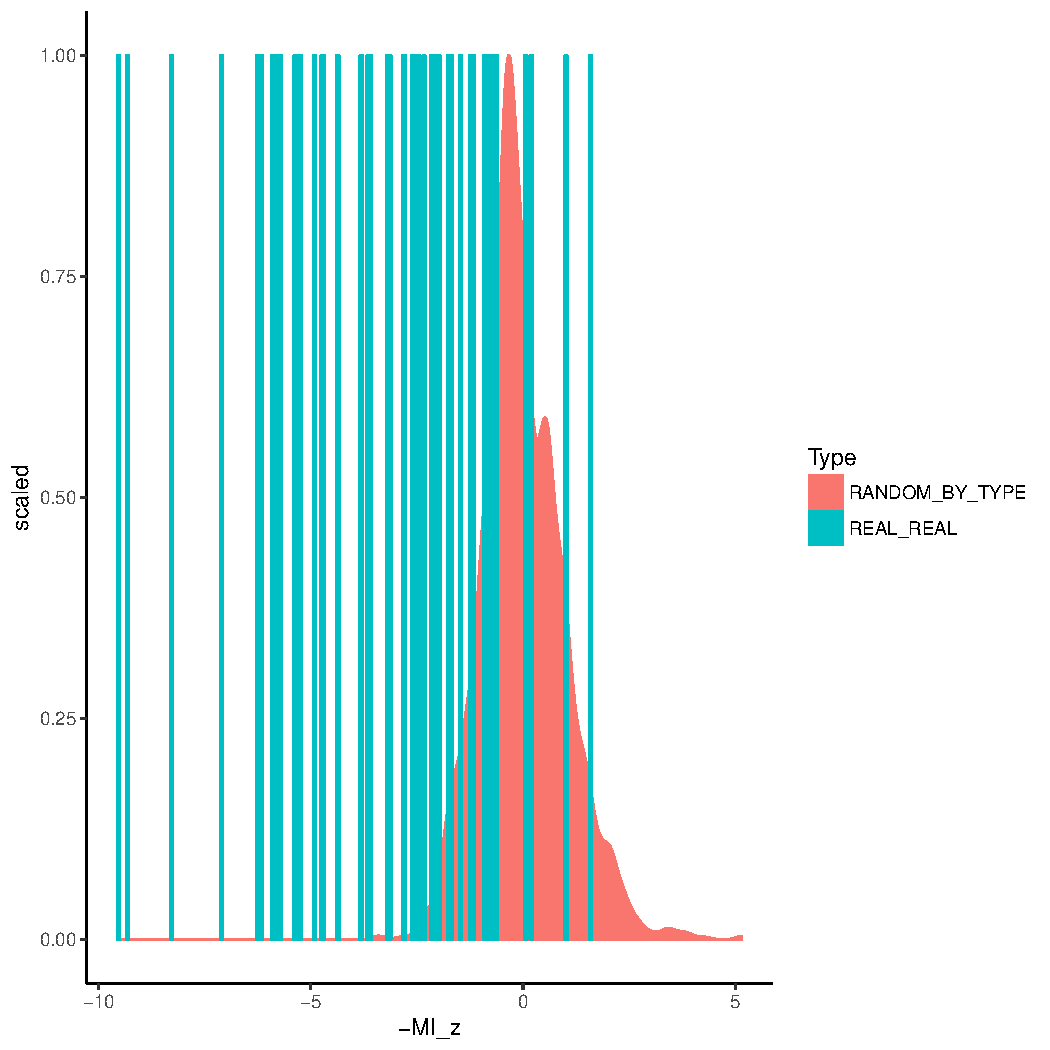
\includegraphics[width=0.5\textwidth]{../code/visualize_neural/figures/full-REAL-listener-surprisal-memory-HIST_z_byMem_onlyWordForms_boundedVocab.pdf}
\caption{Histogram}\label{fig:hist-real}
\end{figure}


\begin{table}[!htbp]
\begin{longtable}{l|ll||l|llllllllllllll}
	Language & Training & Held-Out & 	Language & Training & Held-Out\\ \hline
Afrikaans  &  1,315  &  194  &  Indonesian  &  4,477  &  559  \\
Amharic  &  974  &  100  &  Italian  &  17,427  &  1,070  \\
Arabic  &  21,864  &  2,895  &  Japanese  &  7,164  &  511  \\
Armenian  &  514  &  50  &  Kazakh  &  947  &  100  \\
Bambara  &  926  &  100  &  Korean  &  27,410  &  3,016  \\
Basque  &  5,396  &  1,798  &  Kurmanji  &  634  &  100  \\
Breton  &  788  &  100  &  Latvian  &  4,124  &  989  \\
Bulgarian  &  8,907  &  1,115  &  Maltese  &  1,123  &  433  \\
Buryat  &  808  &  100  &  Naija  &  848  &  100  \\
Cantonese  &  550  &  100  &  North Sami  &  2,257  &  865  \\
Catalan  &  13,123  &  1,709  &  Norwegian  &  29,870  &  4,639  \\
Chinese  &  3,997  &  500  &  Persian  &  4,798  &  599  \\
Croatian  &  7,689  &  600  &  Polish  &  6,100  &  1,027  \\
Czech  &  102,993  &  11,311  &  Portuguese  &  17,995  &  1,770  \\
Danish  &  4,383  &  564  &  Romanian  &  8,664  &  752  \\
Dutch  &  18,310  &  1,518  &  Russian  &  52,664  &  7,163  \\
English  &  17,062  &  3,070  &  Serbian  &  2,935  &  465  \\
Erzya  &  1,450  &  100  &  Slovak  &  8,483  &  1,060  \\
Estonian  &  6,959  &  855  &  Slovenian  &  7,532  &  1,817  \\
Faroese  &  1,108  &  100  &  Spanish  &  28,492  &  3,054  \\
Finnish  &  27,198  &  3,239  &  Swedish  &  7,041  &  1,416  \\
French  &  32,347  &  3,232  &  Thai  &  900  &  100  \\
German  &  13,814  &  799  &  Turkish  &  3,685  &  975  \\
Greek  &  1,662  &  403  &  Ukrainian  &  4,506  &  577  \\
Hebrew  &  5,241  &  484  &  Urdu  &  4,043  &  552  \\
Hindi  &  13,304  &  1,659  &  Uyghur  &  1,656  &  900  \\
Hungarian  &  910  &  441  &  Vietnamese  &  1,400  &  800  \\

\end{longtable}
	\caption{Languages, with the number of training and held-out sentences available.}\label{tab:corpora}
\end{table}

\begin{table}[!htbp]
\begin{longtable}{l|ll||l|llllllllllllll}
	Language & Base. & Real & Language & Base. & Real \\ \hline
Afrikaans  &  13  &  10  &  Indonesian  &  11  &  11  \\
Amharic  &  137  &  10  &  Italian  &  10  &  10  \\
Arabic  &  11  &  10  &  Japanese  &  25  &  15  \\
Armenian  &  140  &  76  &  Kazakh  &  11  &  10  \\
Bambara  &  25  &  29  &  Korean  &  11  &  10  \\
Basque  &  15  &  10  &  Kurmanji  &  338  &  61  \\
Breton  &  35  &  14  &  Latvian  &  308  &  178  \\
Bulgarian  &  14  &  10  &  Maltese  &  30  &  24  \\
Buryat  &  26  &  18  &  Naija  &  214  &  10  \\
Cantonese  &  306  &  32  &  North Sami  &  335  &  194  \\
Catalan  &  11  &  10  &  Norwegian  &  12  &  10  \\
Chinese  &  21  &  10  &  Persian  &  25  &  12  \\
Croatian  &  30  &  17  &  Polish  &  309  &  35  \\
Czech  &  18  &  10  &  Portuguese  &  15  &  55  \\
Danish  &  33  &  17  &  Romanian  &  10  &  10  \\
Dutch  &  27  &  10  &  Russian  &  20  &  10  \\
English  &  13  &  11  &  Serbian  &  26  &  11  \\
Erzya  &  846  &  167  &  Slovak  &  303  &  27  \\
Estonian  &  347  &  101  &  Slovenian  &  297  &  80  \\
Faroese  &  27  &  13  &  Spanish  &  14  &  10  \\
Finnish  &  83  &  16  &  Swedish  &  31  &  14  \\
French  &  14  &  11  &  Thai  &  45  &  19  \\
German  &  19  &  13  &  Turkish  &  13  &  10  \\
Greek  &  16  &  10  &  Ukrainian  &  28  &  18  \\
Hebrew  &  11  &  10  &  Urdu  &  17  &  10  \\
Hindi  &  11  &  10  &  Uyghur  &  326  &  175  \\
Hungarian  &  220  &  109  &  Vietnamese  &  303  &  12  \\

\end{longtable}
	\caption{Samples drawn per language according to the precision-dependent stopping criterion.}\label{tab:samples}
\end{table}



\begin{table}[!htbp]
\begin{longtable}{l|lll||l|lllllllllllllll}
	Language & Mean & Lower & Upper & Language & Mean & Lower & Upper \\ \hline
Afrikaans  &  1.0  &  1.0  &  1.0  &  Indonesian  &  1.0  &  1.0  &  1.0  \\
Amharic  &  1.0  &  1.0  &  1.0  &  Italian  &  1.0  &  1.0  &  1.0  \\
Arabic  &  1.0  &  1.0  &  1.0  &  Japanese  &  1.0  &  1.0  &  1.0  \\
Armenian  &  0.92  &  0.87  &  0.97  &  Kazakh  &  1.0  &  1.0  &  1.0  \\
Bambara  &  1.0  &  1.0  &  1.0  &  Korean  &  1.0  &  1.0  &  1.0  \\
Basque  &  1.0  &  1.0  &  1.0  &  Kurmanji  &  0.93  &  0.88  &  0.98  \\
Breton  &  1.0  &  1.0  &  1.0  &  Latvian  &  0.49  &  0.4  &  0.57  \\
Bulgarian  &  1.0  &  1.0  &  1.0  &  Maltese  &  1.0  &  1.0  &  1.0  \\
Buryat  &  1.0  &  1.0  &  1.0  &  Naija  &  1.0  &  0.99  &  1.0  \\
Cantonese  &  0.96  &  0.86  &  1.0  &  North Sami  &  0.37  &  0.3  &  0.44  \\
Catalan  &  1.0  &  1.0  &  1.0  &  Norwegian  &  1.0  &  1.0  &  1.0  \\
Chinese  &  1.0  &  1.0  &  1.0  &  Persian  &  1.0  &  1.0  &  1.0  \\
Croatian  &  1.0  &  1.0  &  1.0  &  Polish  &  0.1  &  0.04  &  0.17  \\
Czech  &  1.0  &  1.0  &  1.0  &  Portuguese  &  1.0  &  1.0  &  1.0  \\
Danish  &  1.0  &  1.0  &  1.0  &  Romanian  &  1.0  &  1.0  &  1.0  \\
Dutch  &  1.0  &  1.0  &  1.0  &  Russian  &  1.0  &  1.0  &  1.0  \\
English  &  1.0  &  1.0  &  1.0  &  Serbian  &  1.0  &  1.0  &  1.0  \\
Erzya  &  0.99  &  0.98  &  1.0  &  Slovak  &  0.07  &  0.03  &  0.12  \\
Estonian  &  0.8  &  0.72  &  0.86  &  Slovenian  &  0.82  &  0.77  &  0.88  \\
Faroese  &  1.0  &  1.0  &  1.0  &  Spanish  &  1.0  &  1.0  &  1.0  \\
Finnish  &  1.0  &  1.0  &  1.0  &  Swedish  &  1.0  &  1.0  &  1.0  \\
French  &  1.0  &  1.0  &  1.0  &  Thai  &  1.0  &  1.0  &  1.0  \\
German  &  1.0  &  0.91  &  1.0  &  Turkish  &  1.0  &  1.0  &  1.0  \\
Greek  &  1.0  &  1.0  &  1.0  &  Ukrainian  &  1.0  &  1.0  &  1.0  \\
Hebrew  &  1.0  &  1.0  &  1.0  &  Urdu  &  1.0  &  1.0  &  1.0  \\
Hindi  &  1.0  &  1.0  &  1.0  &  Uyghur  &  0.65  &  0.57  &  0.73  \\
Hungarian  &  0.87  &  0.8  &  0.93  &  Vietnamese  &  1.0  &  0.98  &  1.0  \\

\end{longtable}
	\caption{Bootstrapped estimates for $G$.}\label{tab:boot-g}
\end{table}



\begin{table}[!htbp]
\begin{longtable}{ccccccccccccccclll}
Afrikaans & Amharic & Arabic & Armenian
 \\ 
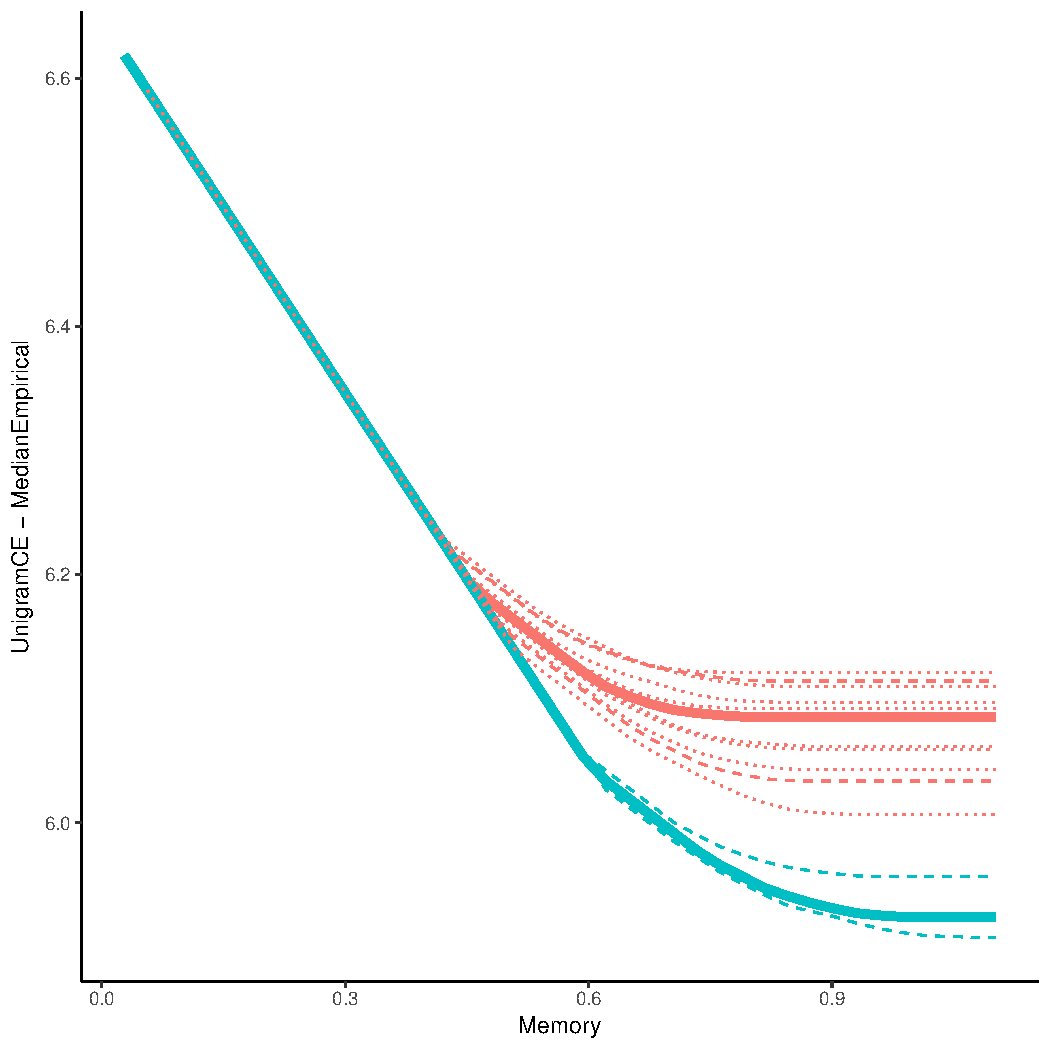
\includegraphics[width=0.25\textwidth]{neural/figures/Afrikaans-listener-surprisal-memory-MEDIANS_QUANTILES_onlyWordForms_boundedVocab_REAL.pdf} & 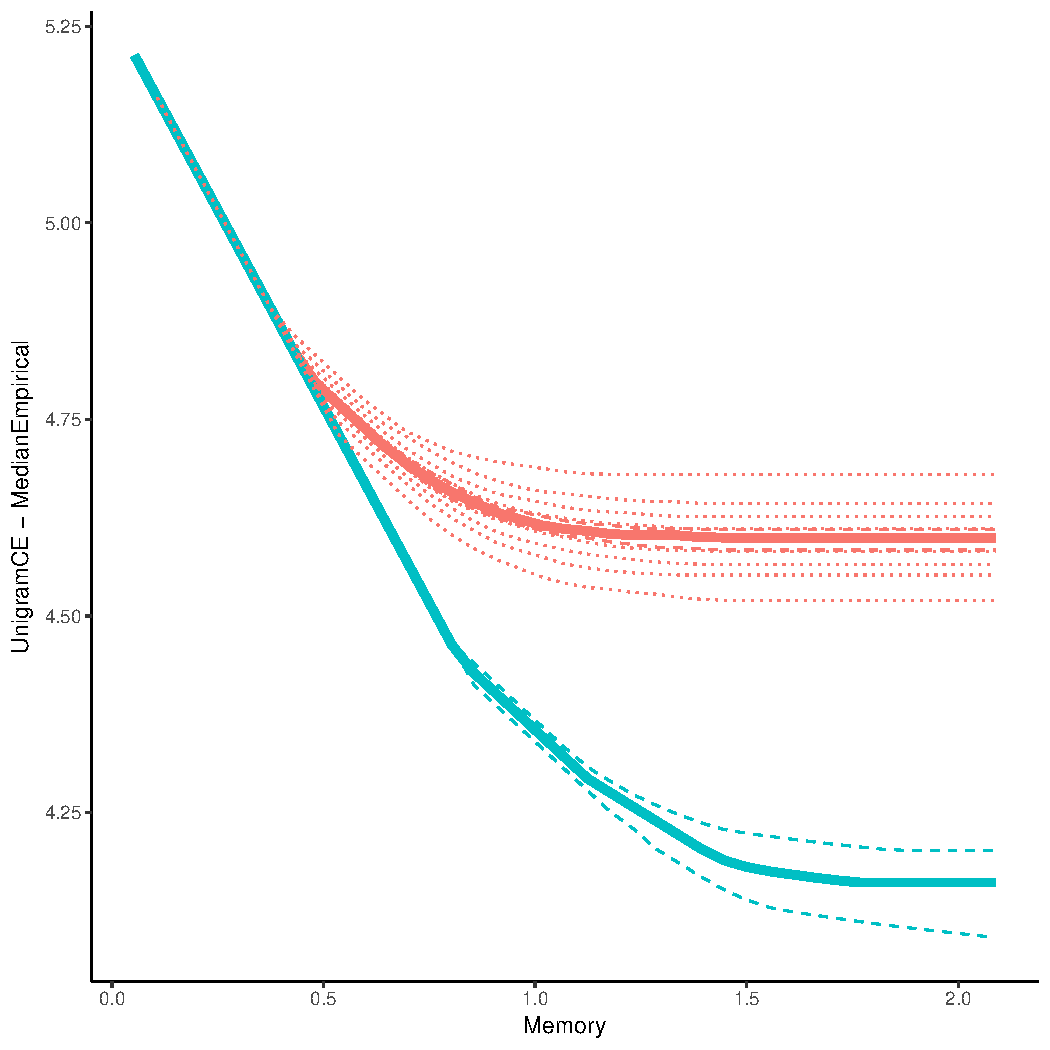
\includegraphics[width=0.25\textwidth]{neural/figures/Amharic-Adap-listener-surprisal-memory-MEDIANS_QUANTILES_onlyWordForms_boundedVocab_REAL.pdf} & 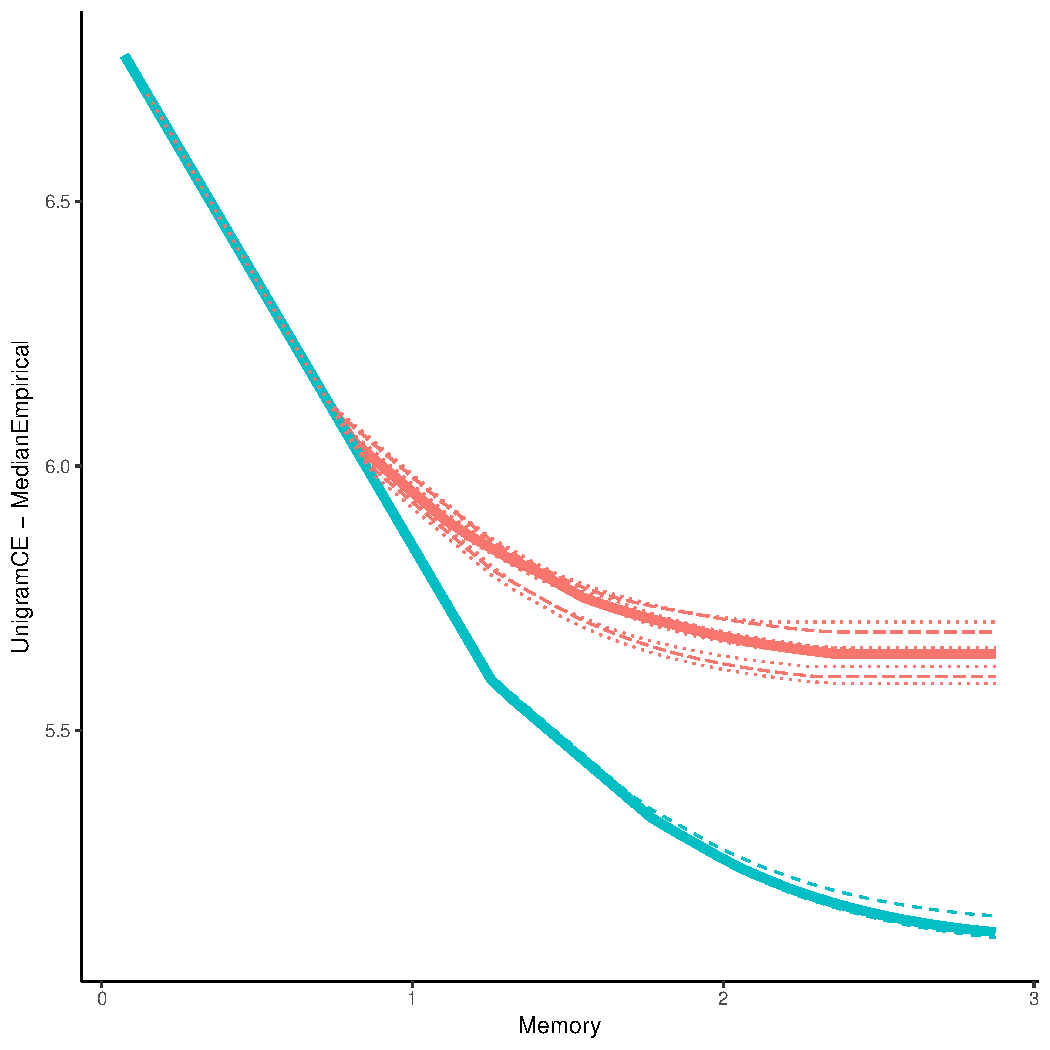
\includegraphics[width=0.25\textwidth]{neural/figures/Arabic-listener-surprisal-memory-MEDIANS_QUANTILES_onlyWordForms_boundedVocab_REAL.pdf} & 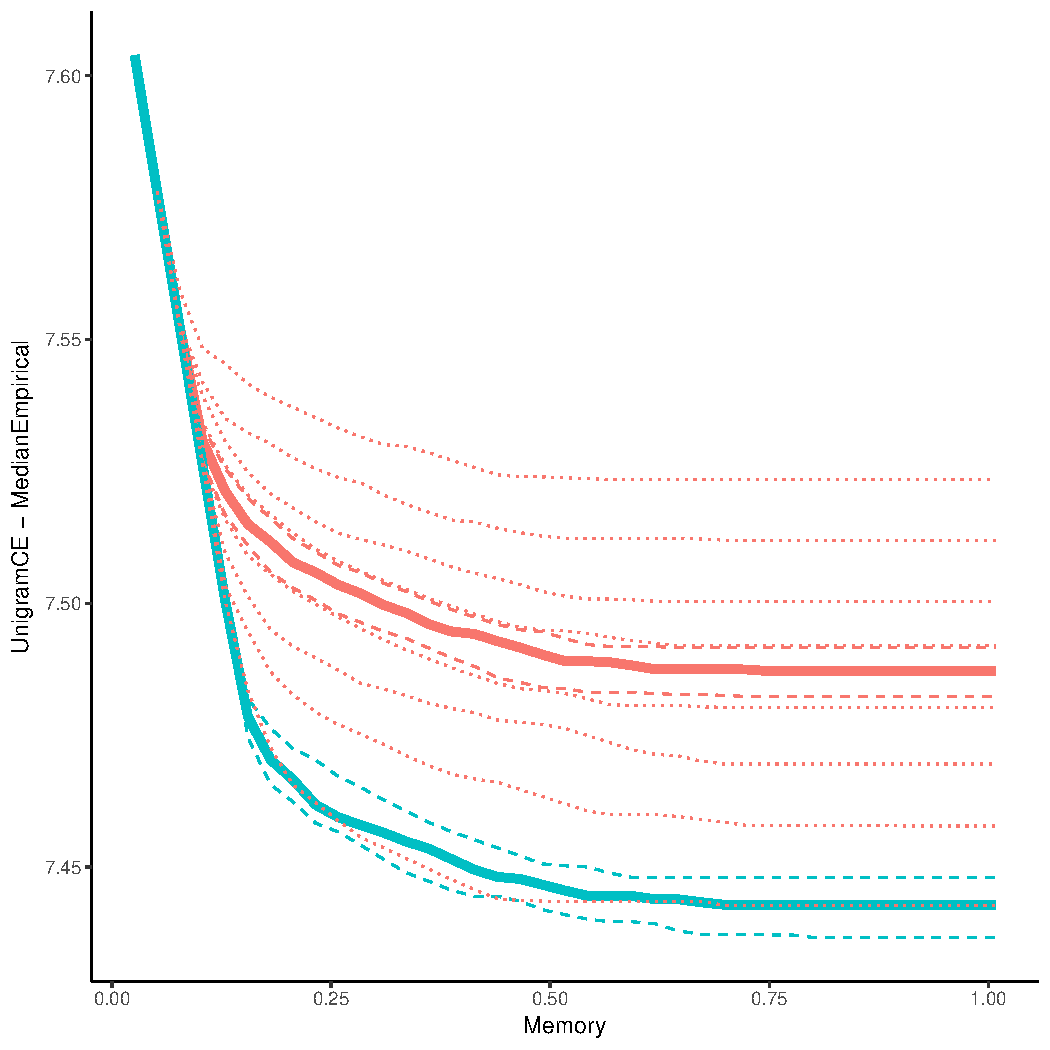
\includegraphics[width=0.25\textwidth]{neural/figures/Armenian-Adap-listener-surprisal-memory-MEDIANS_QUANTILES_onlyWordForms_boundedVocab_REAL.pdf}
 \\ 
Bambara & Basque & Breton & Bulgarian
 \\ 
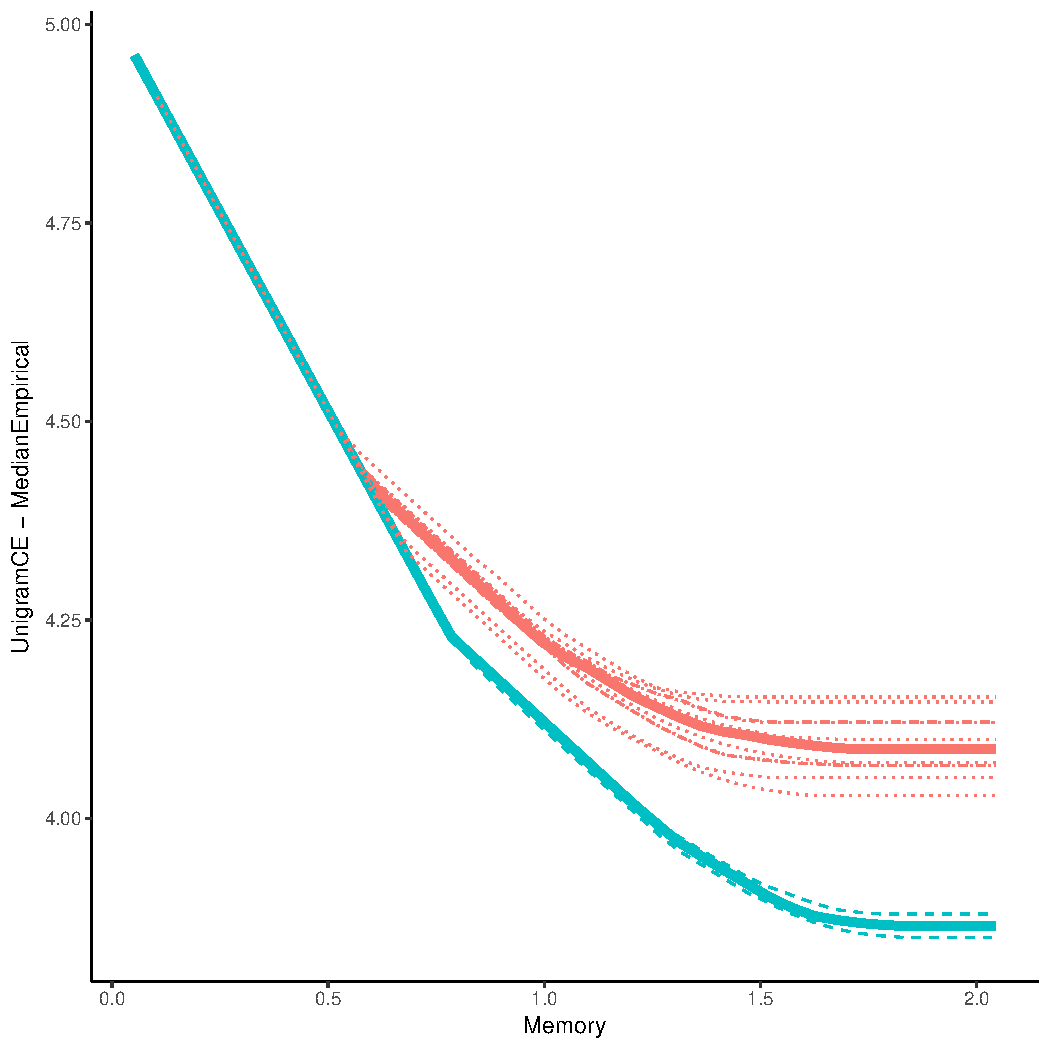
\includegraphics[width=0.25\textwidth]{neural/figures/Bambara-Adap-listener-surprisal-memory-MEDIANS_QUANTILES_onlyWordForms_boundedVocab_REAL.pdf} & 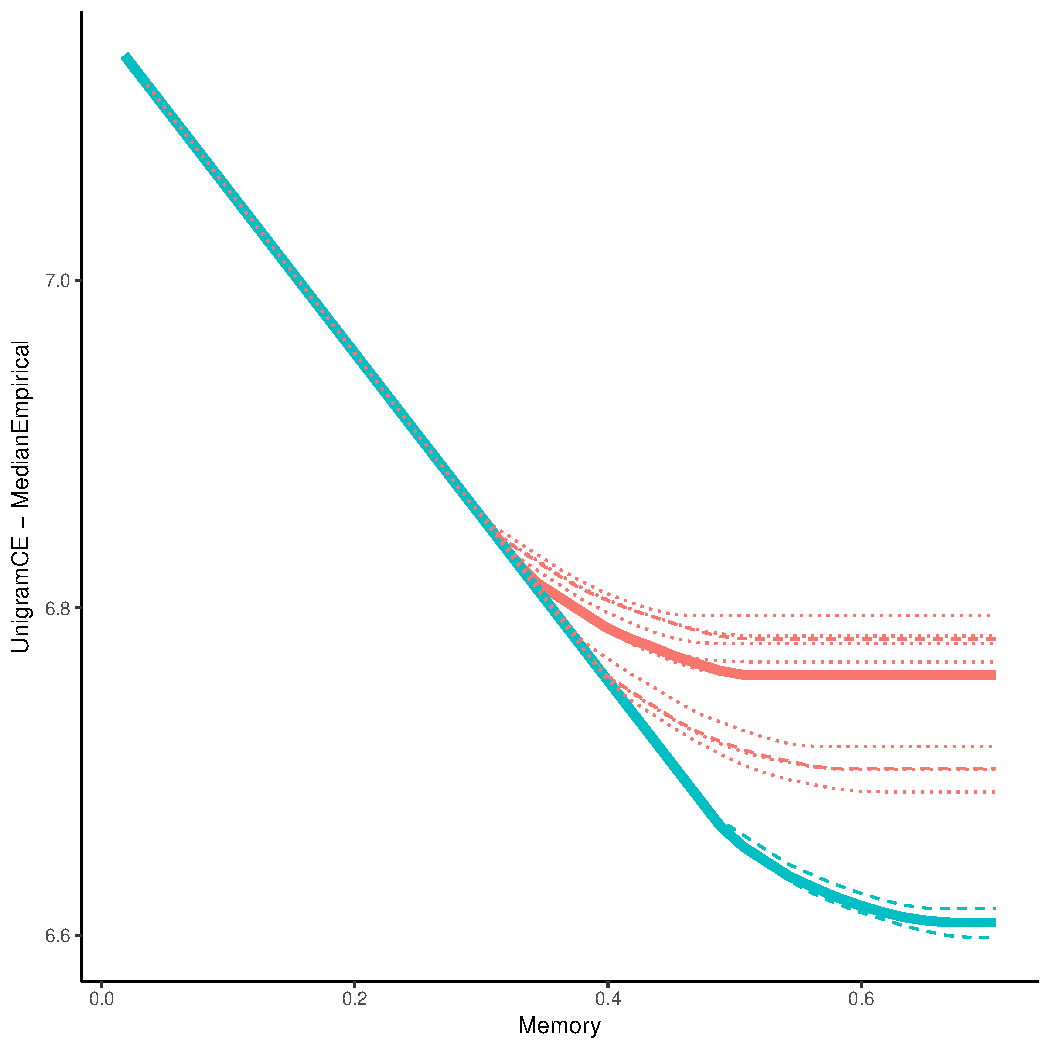
\includegraphics[width=0.25\textwidth]{neural/figures/Basque-listener-surprisal-memory-MEDIANS_QUANTILES_onlyWordForms_boundedVocab_REAL.pdf} & 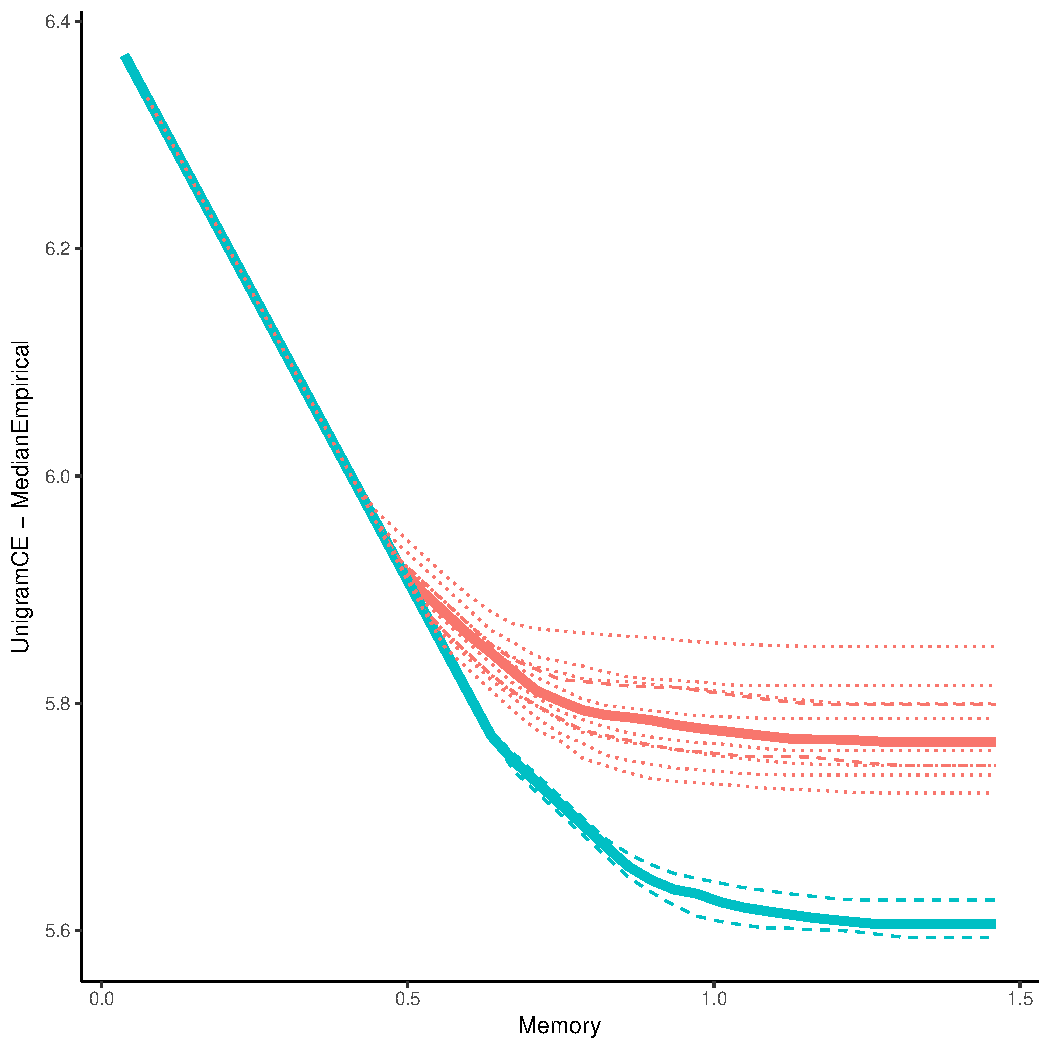
\includegraphics[width=0.25\textwidth]{neural/figures/Breton-Adap-listener-surprisal-memory-MEDIANS_QUANTILES_onlyWordForms_boundedVocab_REAL.pdf} & 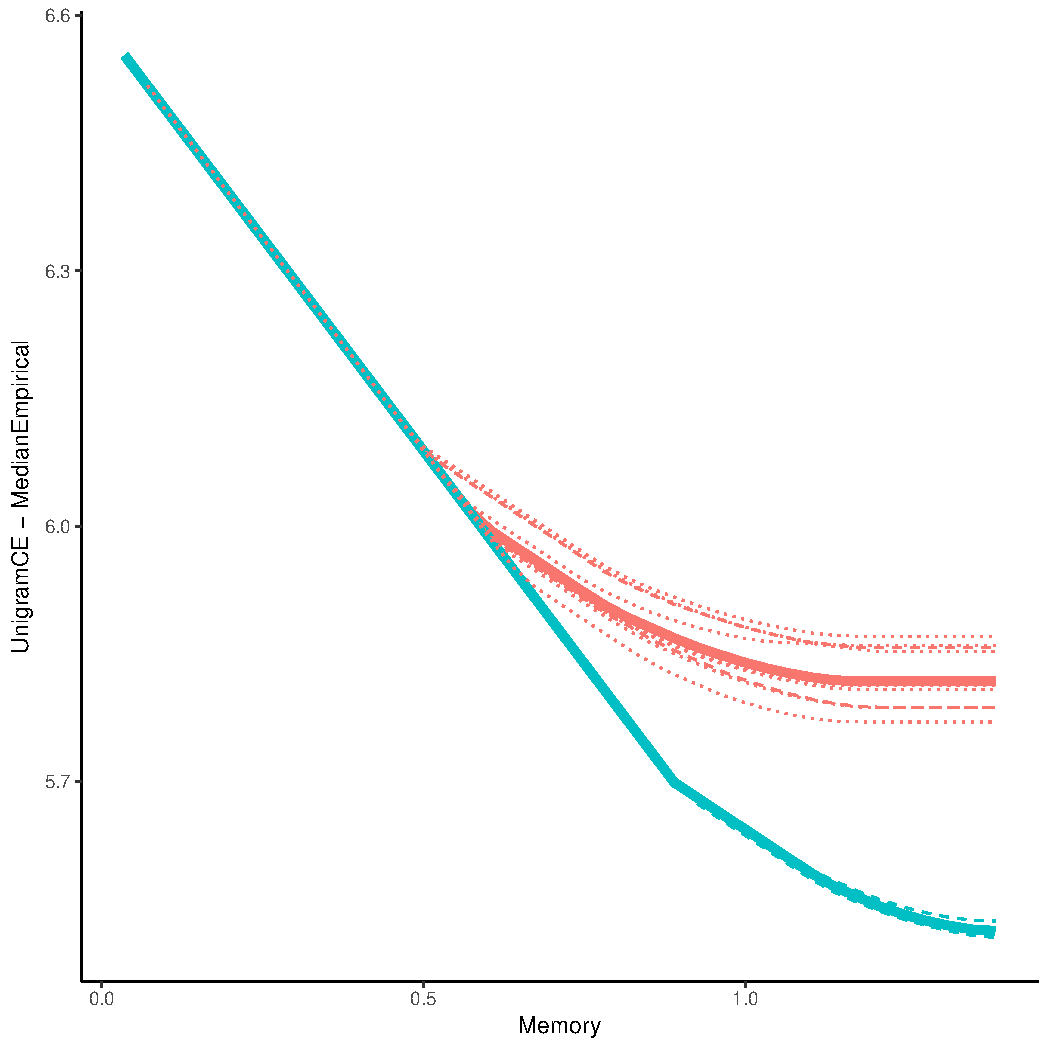
\includegraphics[width=0.25\textwidth]{neural/figures/Bulgarian-listener-surprisal-memory-MEDIANS_QUANTILES_onlyWordForms_boundedVocab_REAL.pdf}
 \\ 
Buryat & Cantonese & Catalan & Chinese
 \\ 
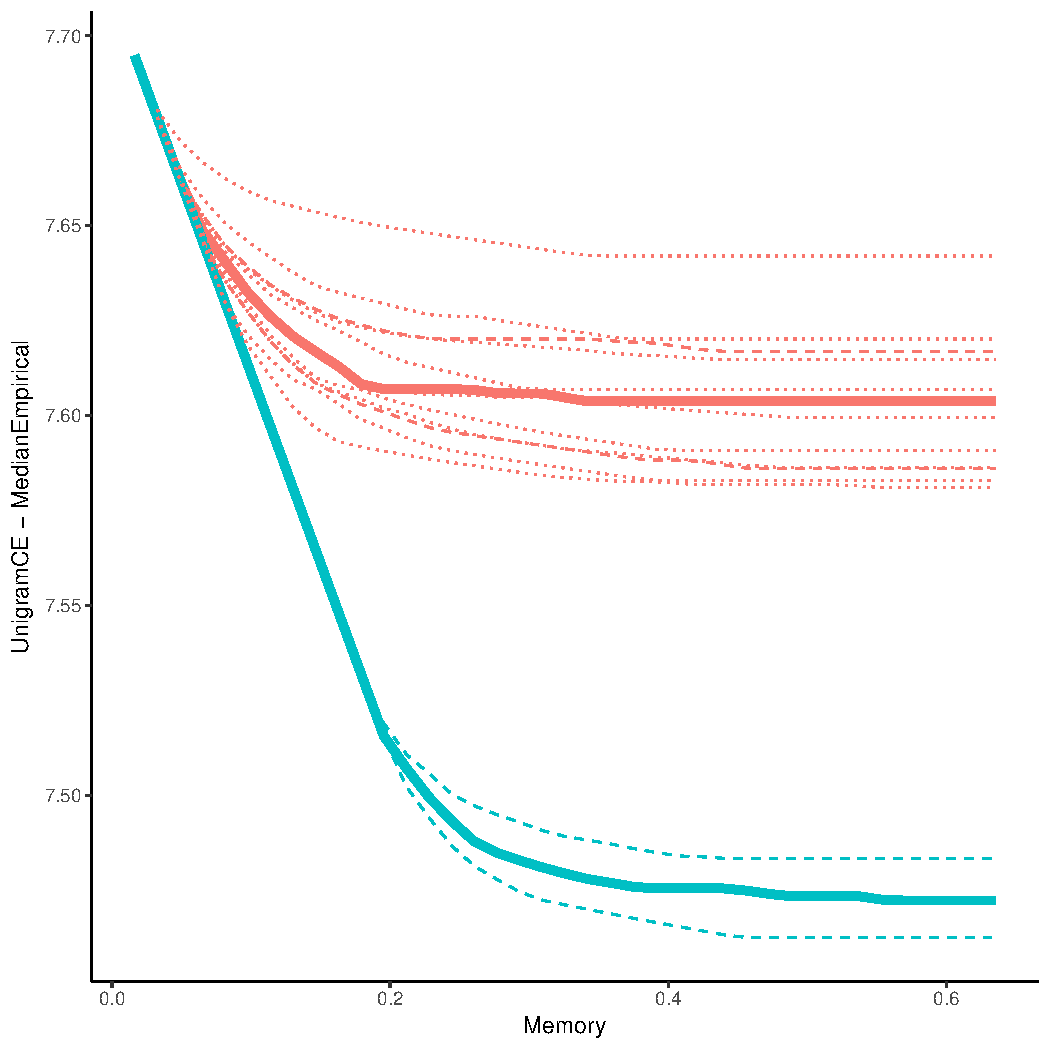
\includegraphics[width=0.25\textwidth]{neural/figures/Buryat-Adap-listener-surprisal-memory-MEDIANS_QUANTILES_onlyWordForms_boundedVocab_REAL.pdf} & 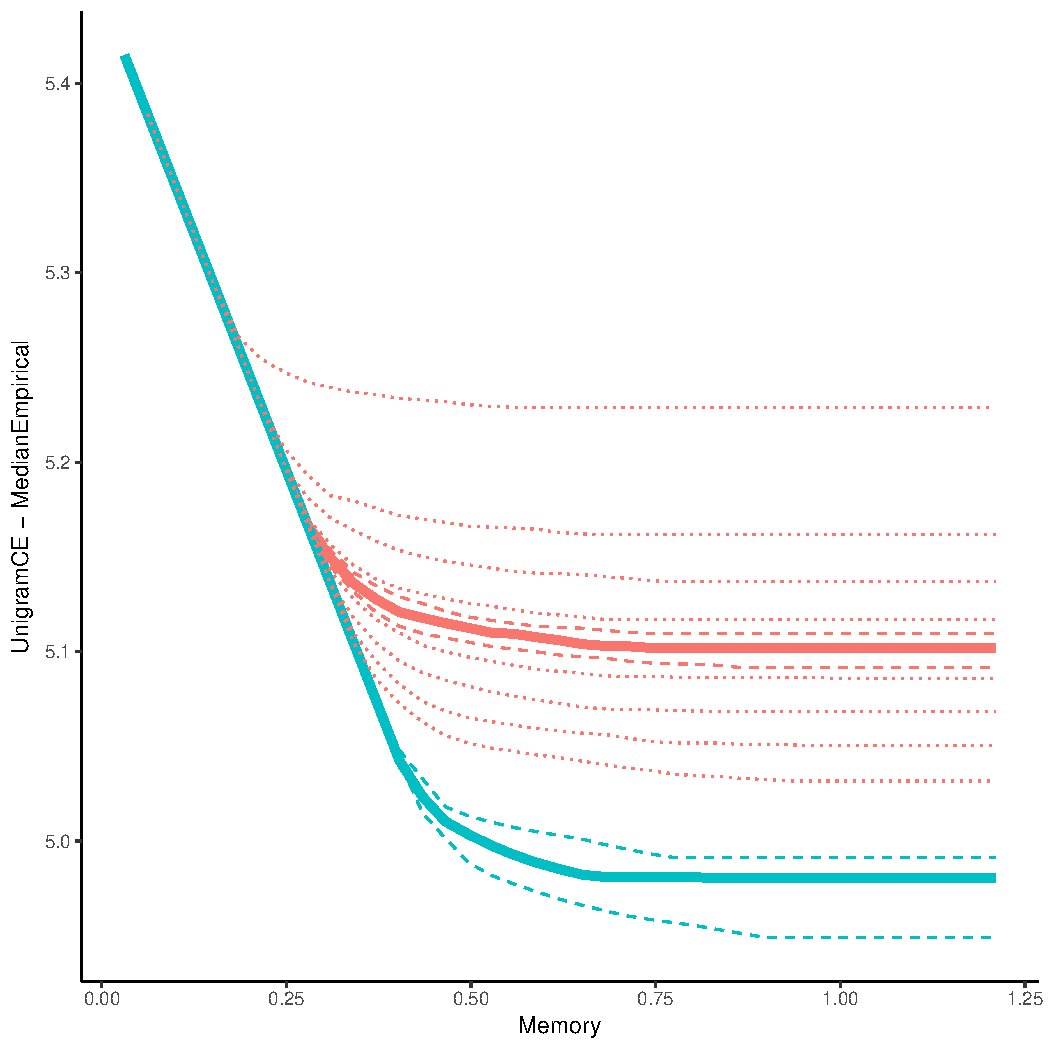
\includegraphics[width=0.25\textwidth]{neural/figures/Cantonese-Adap-listener-surprisal-memory-MEDIANS_QUANTILES_onlyWordForms_boundedVocab_REAL.pdf} & 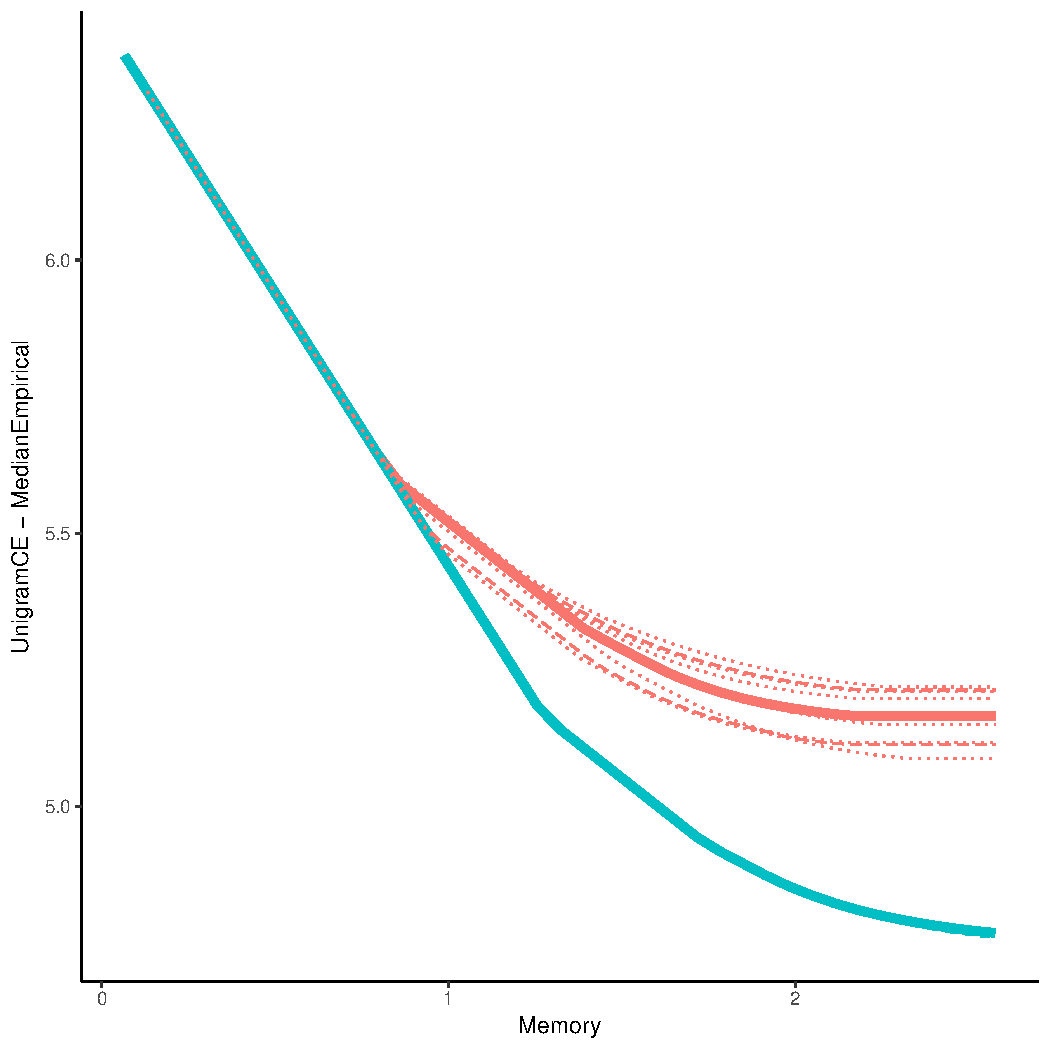
\includegraphics[width=0.25\textwidth]{neural/figures/Catalan-listener-surprisal-memory-MEDIANS_QUANTILES_onlyWordForms_boundedVocab_REAL.pdf} & 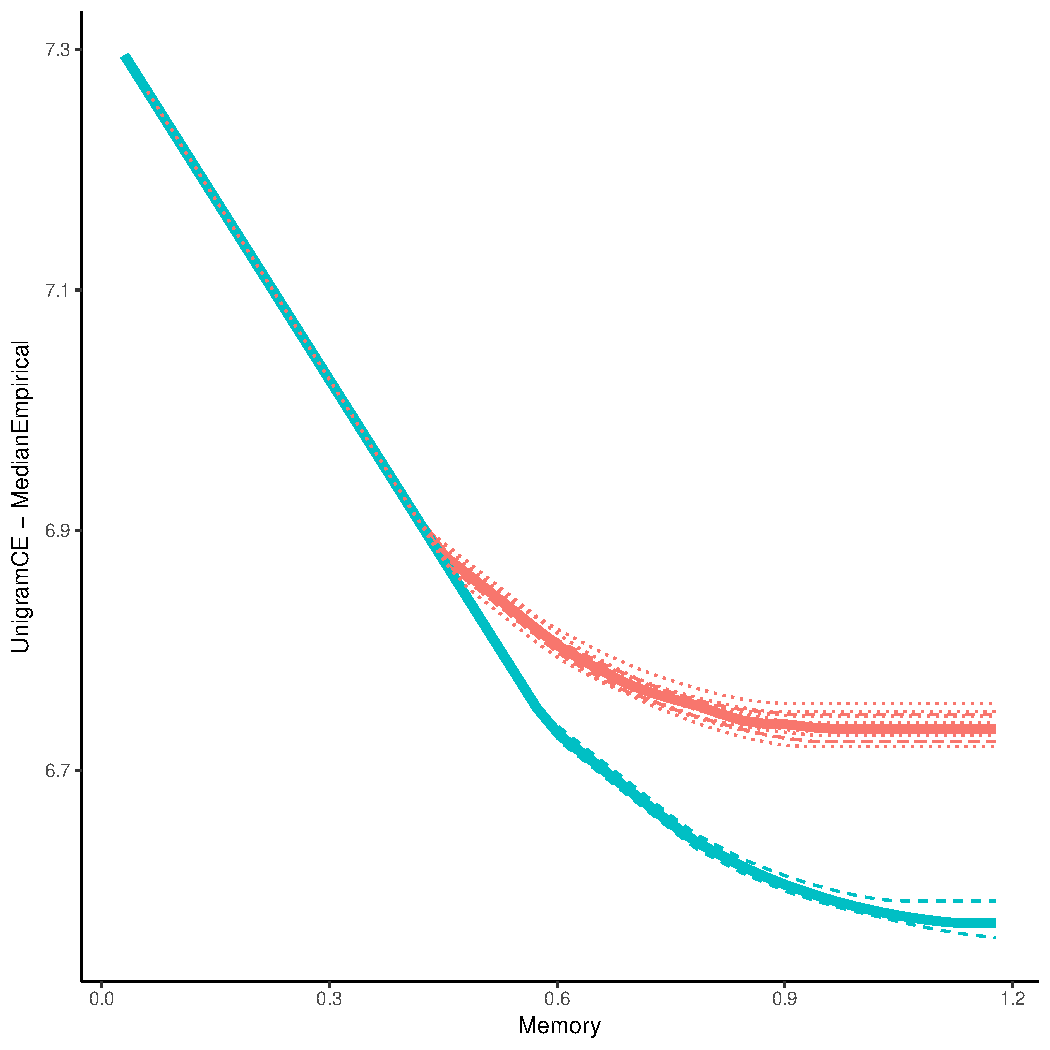
\includegraphics[width=0.25\textwidth]{neural/figures/Chinese-listener-surprisal-memory-MEDIANS_QUANTILES_onlyWordForms_boundedVocab_REAL.pdf}
 \\ 
Croatian & Czech & Danish & Dutch
 \\ 
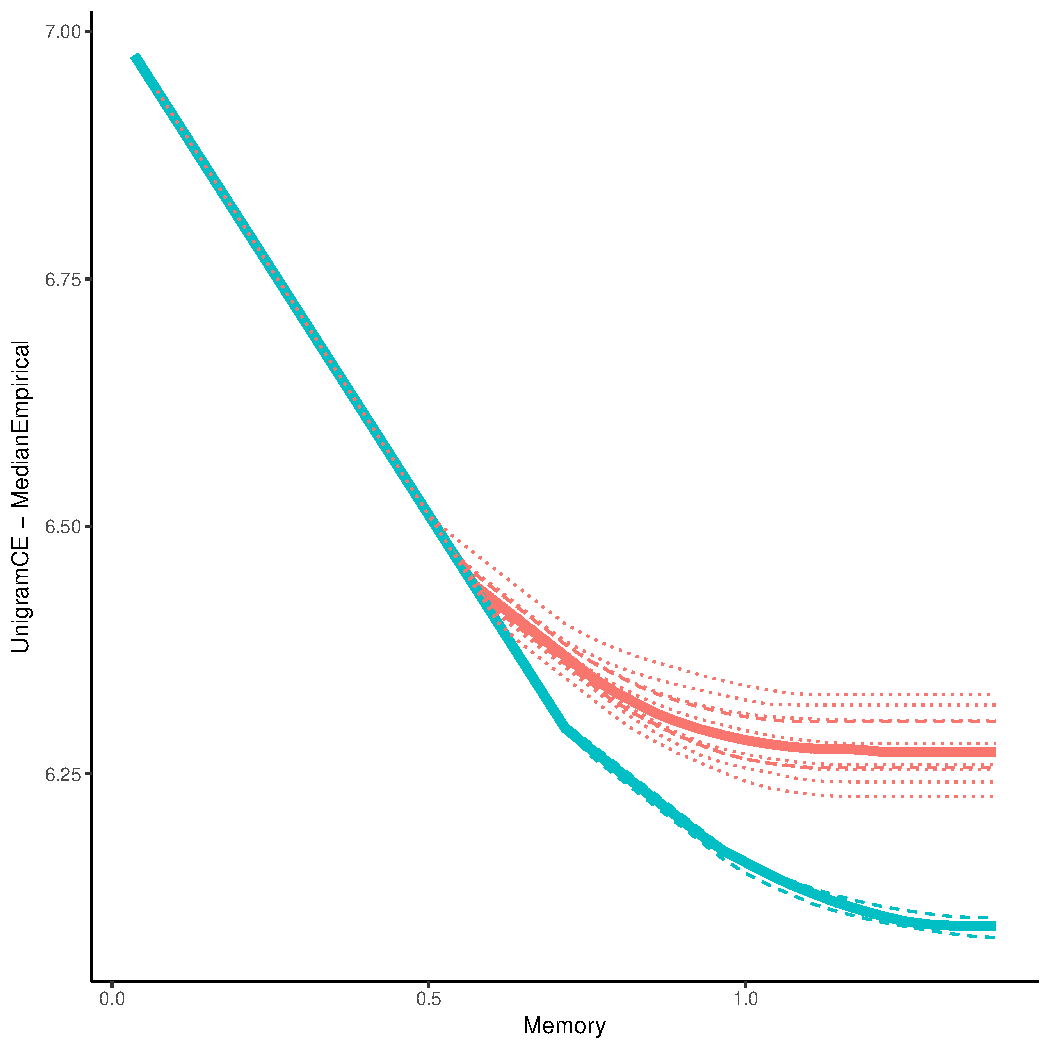
\includegraphics[width=0.25\textwidth]{neural/figures/Croatian-listener-surprisal-memory-MEDIANS_QUANTILES_onlyWordForms_boundedVocab_REAL.pdf} & 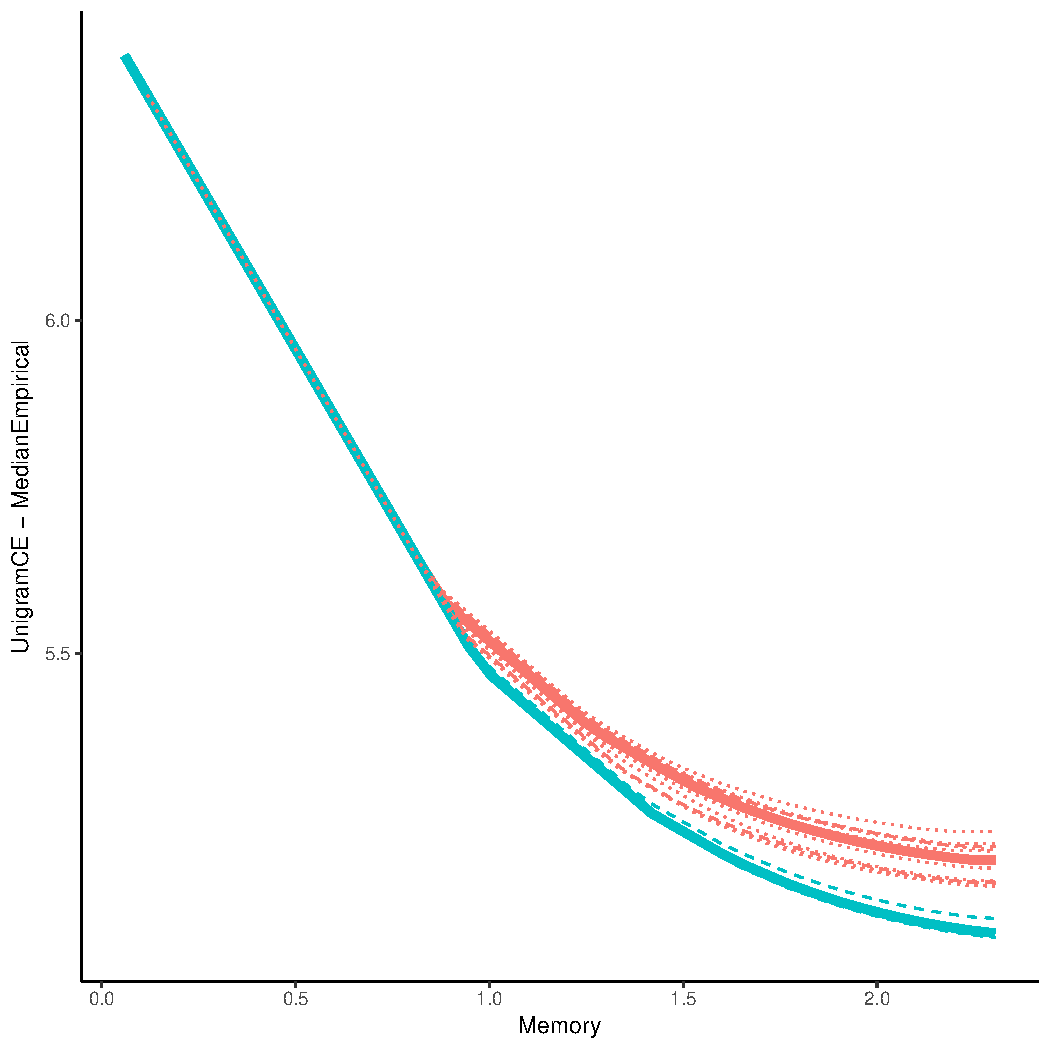
\includegraphics[width=0.25\textwidth]{neural/figures/Czech-listener-surprisal-memory-MEDIANS_QUANTILES_onlyWordForms_boundedVocab_REAL.pdf} & 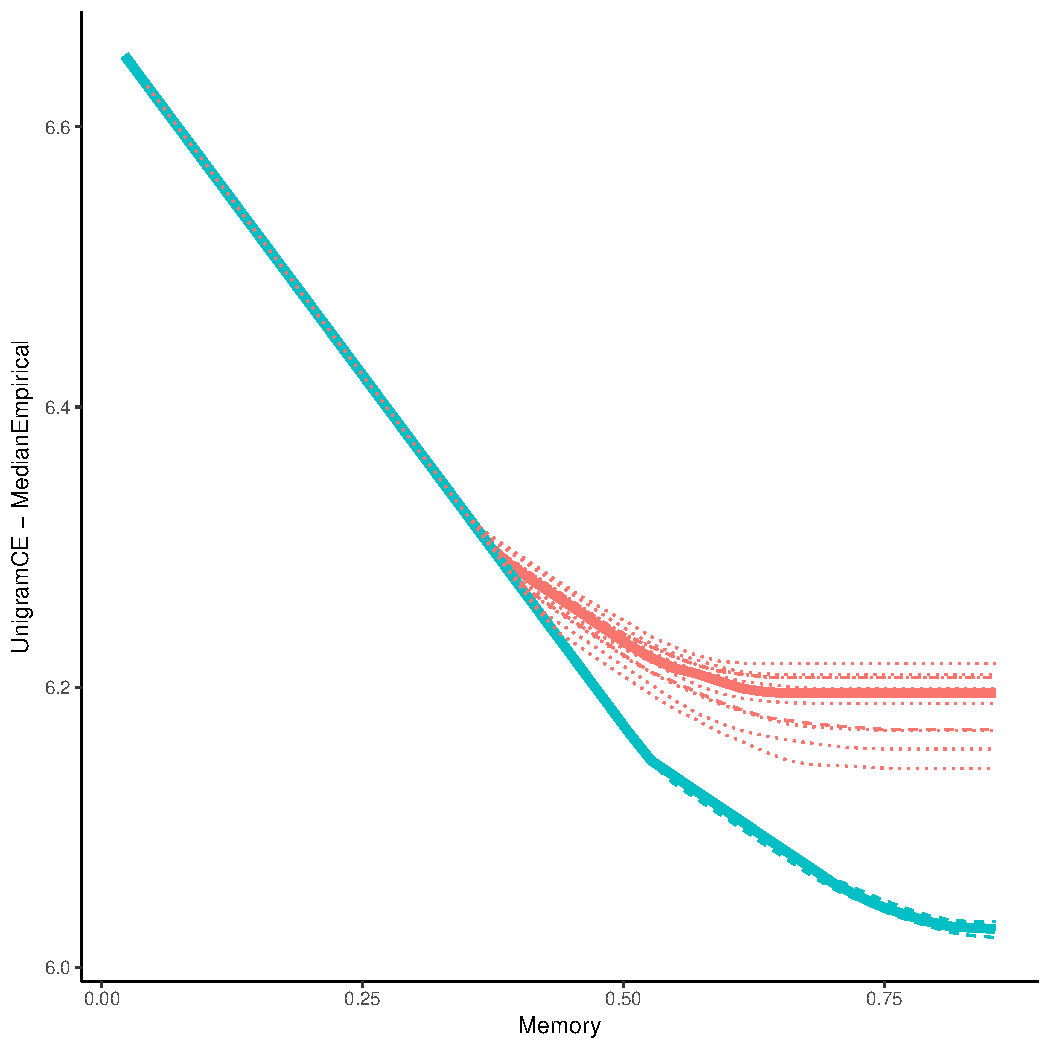
\includegraphics[width=0.25\textwidth]{neural/figures/Danish-listener-surprisal-memory-MEDIANS_QUANTILES_onlyWordForms_boundedVocab_REAL.pdf} & 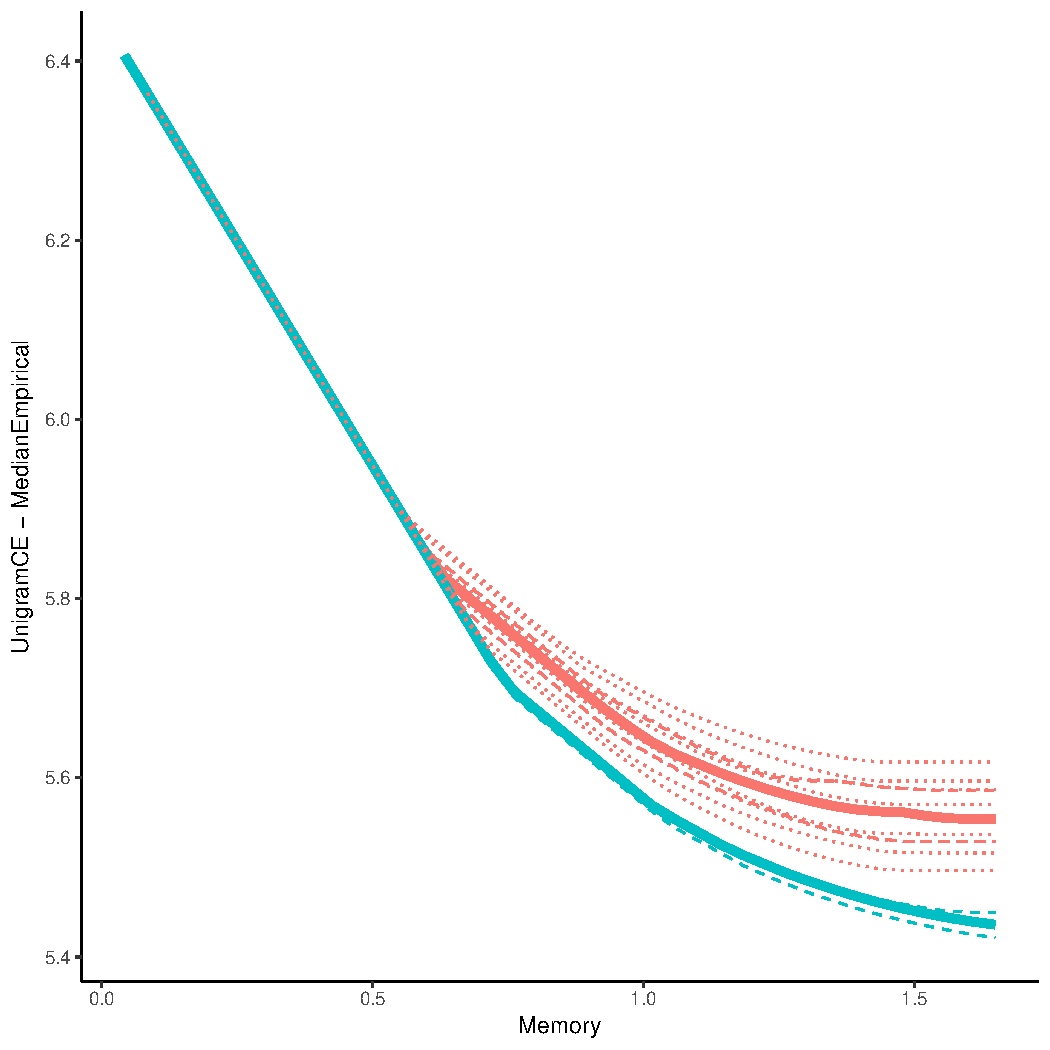
\includegraphics[width=0.25\textwidth]{neural/figures/Dutch-listener-surprisal-memory-MEDIANS_QUANTILES_onlyWordForms_boundedVocab_REAL.pdf}
 \\ 

\end{longtable}
	\caption{Medians: For each memory budget, we provide the median surprisal for real and random languages. Solid lines indicate sample medians, dashed lines indicate 95 $\%$ confidence intervals for the population median, dotted lines indicate empirical quantiles ($10\%, 20\%, \dots, 80\%, 90\%$). Green: Random baselines; blue: real language; red: maximum-likelihood grammars fit to real orderings.}\label{tab:medians}
\end{table}

\begin{table}[!htbp]
\begin{longtable}{ccccccccccccccclll}
English & Erzya & Estonian & Faroese
 \\ 
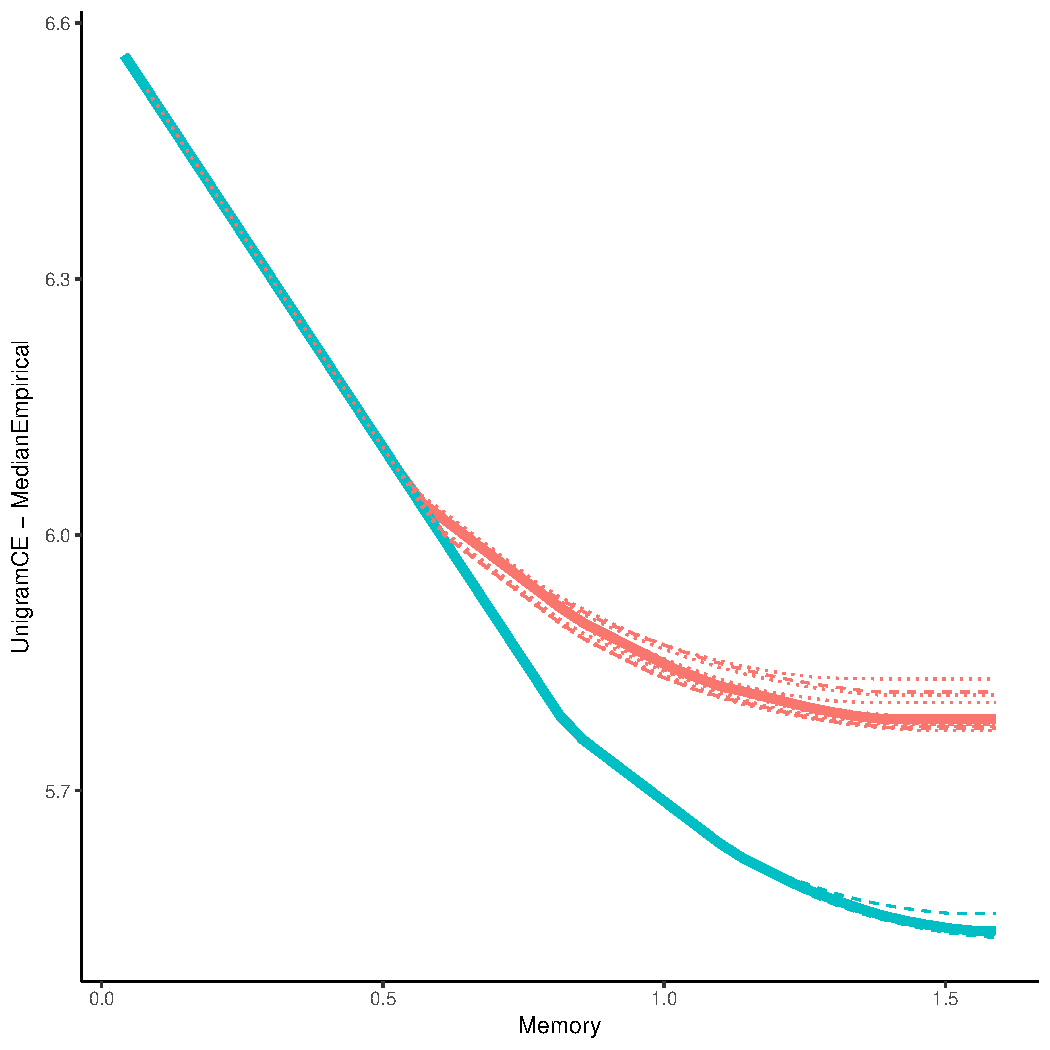
\includegraphics[width=0.25\textwidth]{neural/figures/English-listener-surprisal-memory-MEDIANS_QUANTILES_onlyWordForms_boundedVocab_REAL.pdf} & 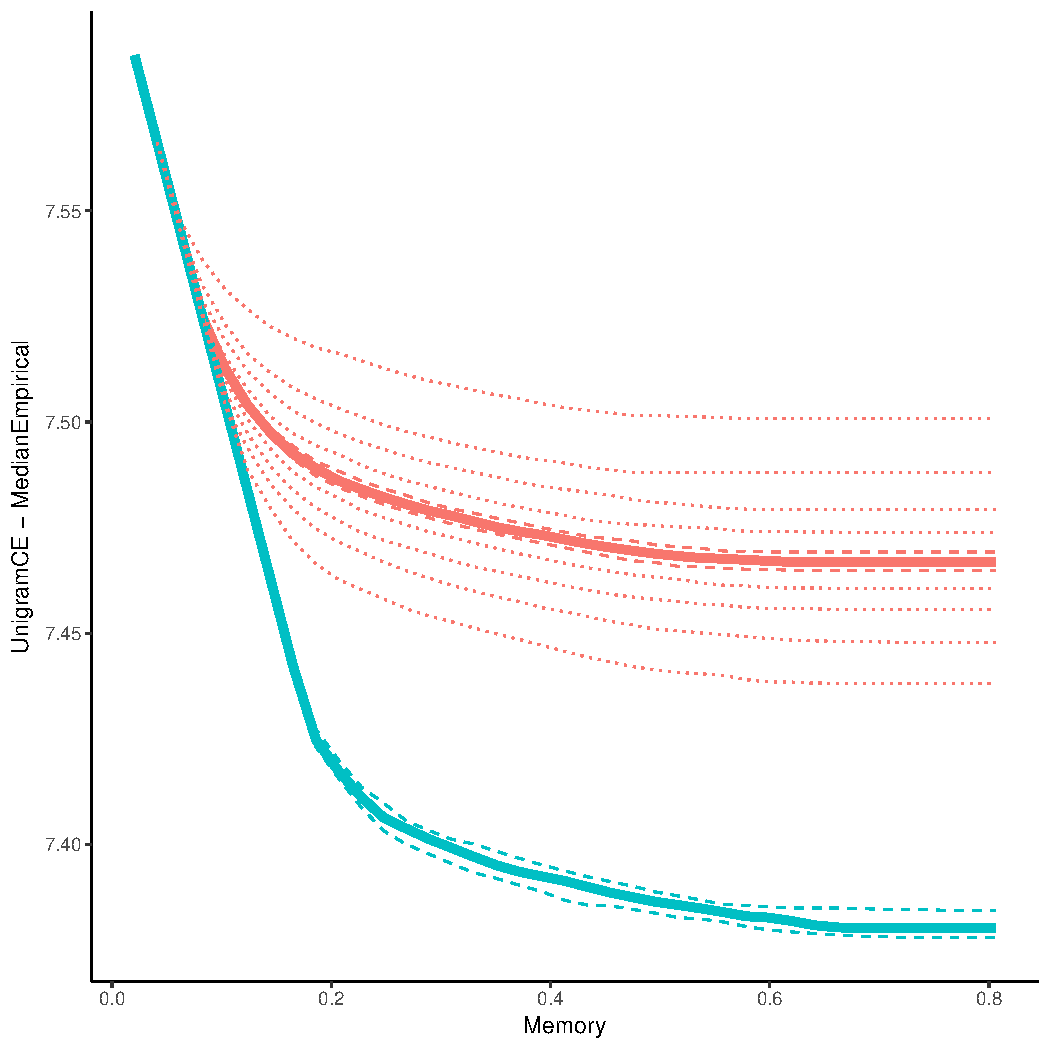
\includegraphics[width=0.25\textwidth]{neural/figures/Erzya-Adap-listener-surprisal-memory-MEDIANS_QUANTILES_onlyWordForms_boundedVocab_REAL.pdf} & 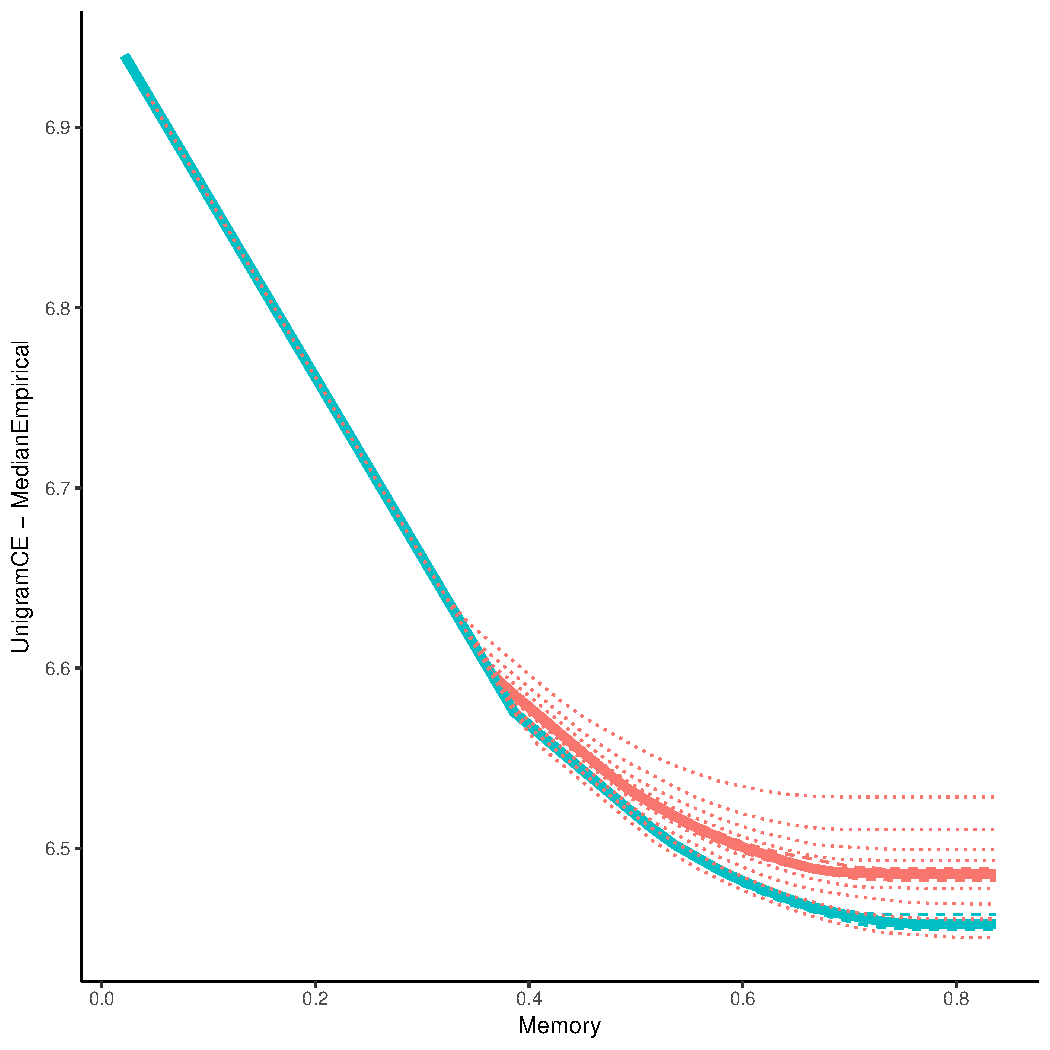
\includegraphics[width=0.25\textwidth]{neural/figures/Estonian-listener-surprisal-memory-MEDIANS_QUANTILES_onlyWordForms_boundedVocab_REAL.pdf} & 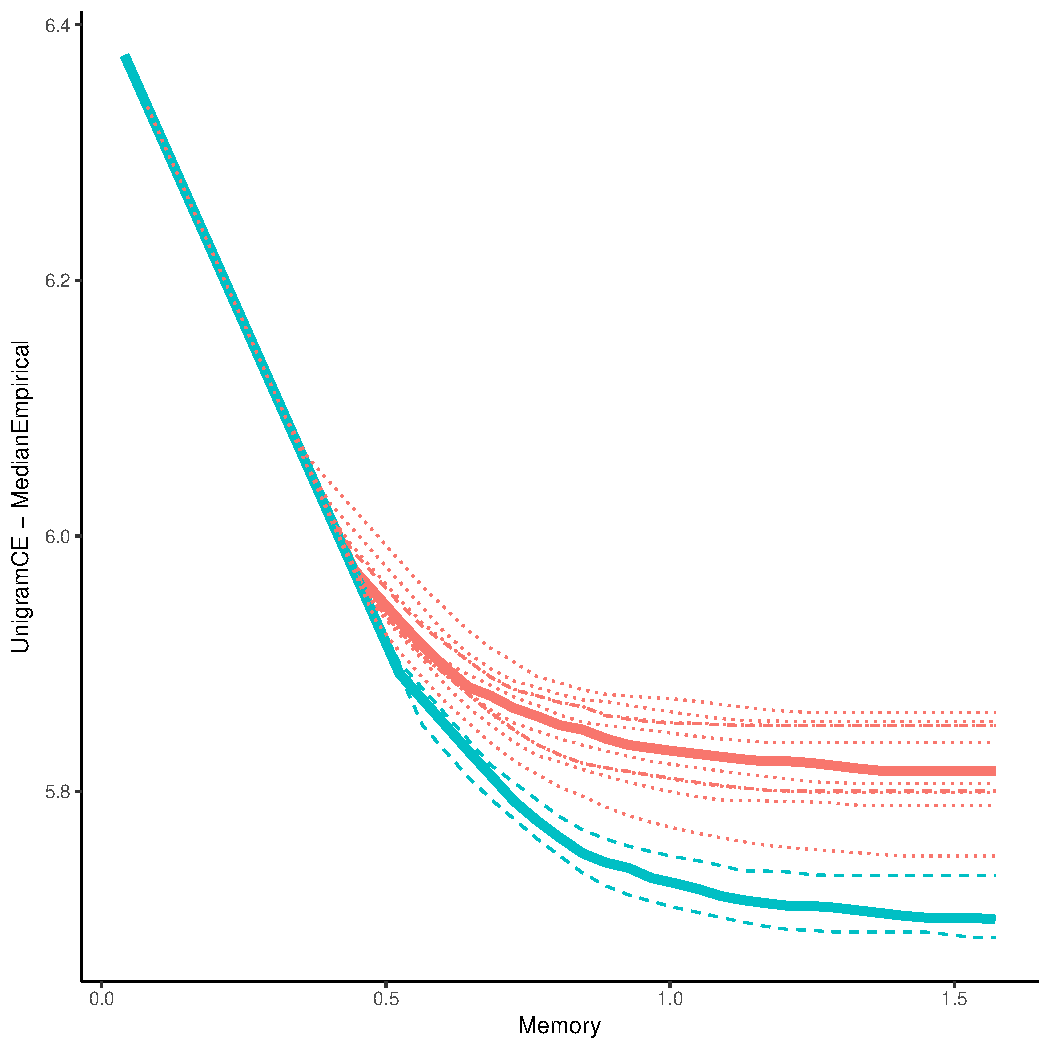
\includegraphics[width=0.25\textwidth]{neural/figures/Faroese-Adap-listener-surprisal-memory-MEDIANS_QUANTILES_onlyWordForms_boundedVocab_REAL.pdf}
 \\ 
Finnish & French & German & Greek
 \\ 
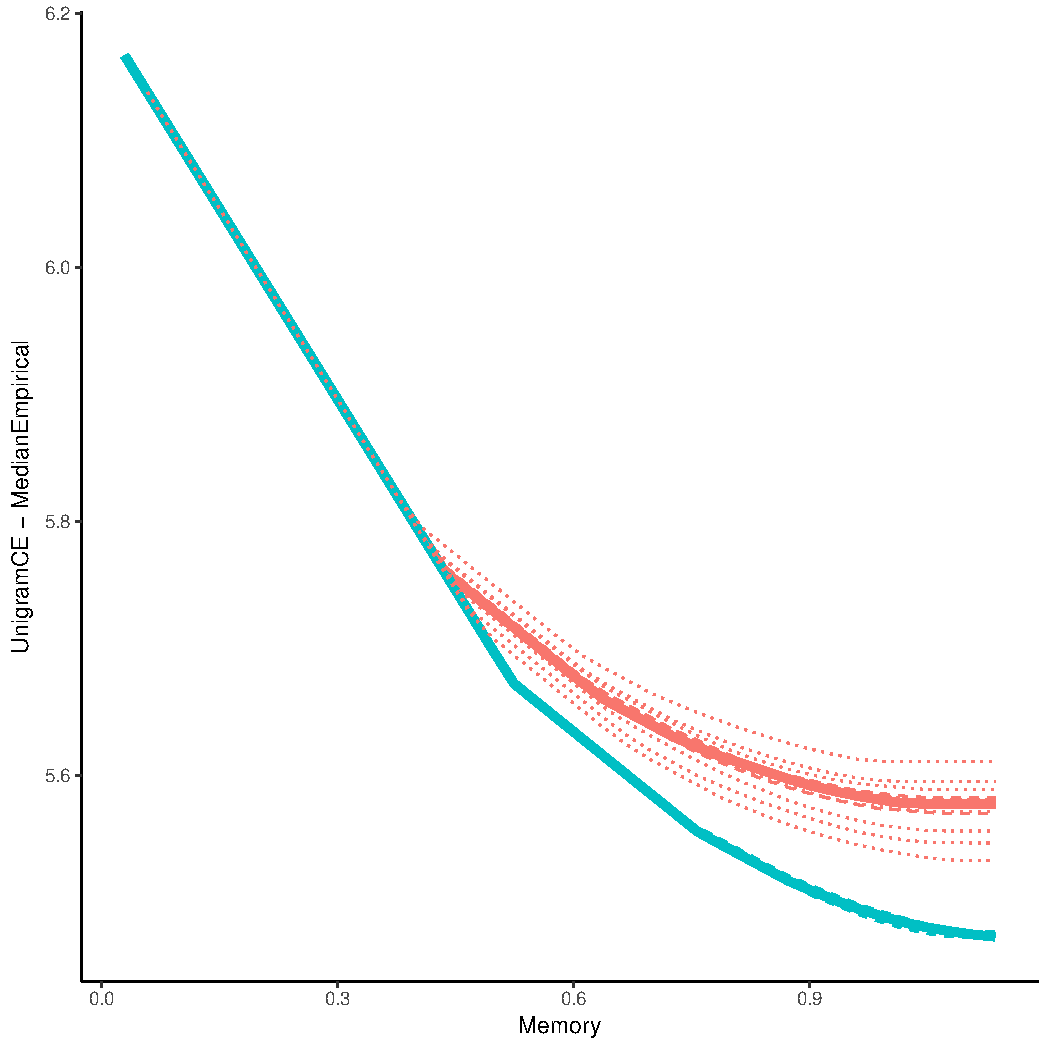
\includegraphics[width=0.25\textwidth]{neural/figures/Finnish-listener-surprisal-memory-MEDIANS_QUANTILES_onlyWordForms_boundedVocab_REAL.pdf} & 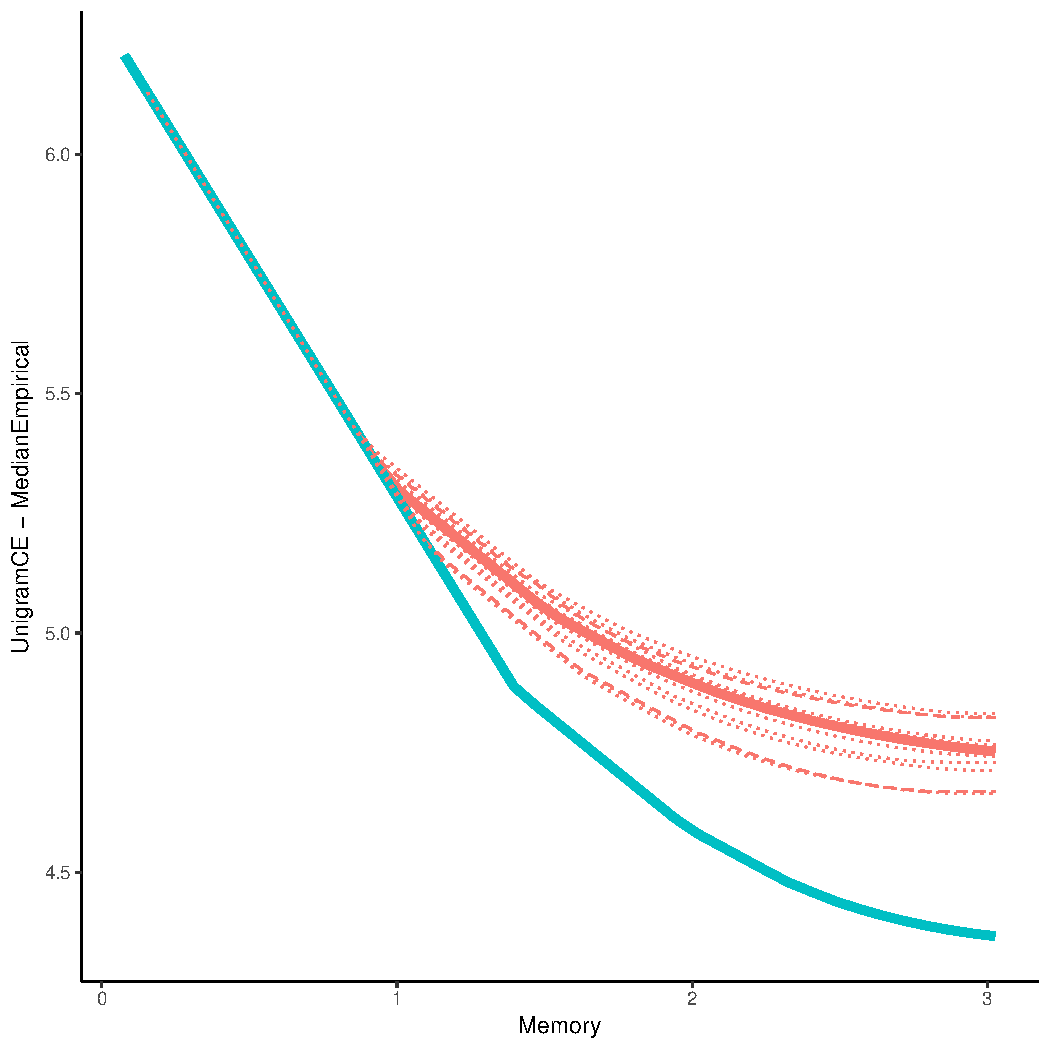
\includegraphics[width=0.25\textwidth]{neural/figures/French-listener-surprisal-memory-MEDIANS_QUANTILES_onlyWordForms_boundedVocab_REAL.pdf} & 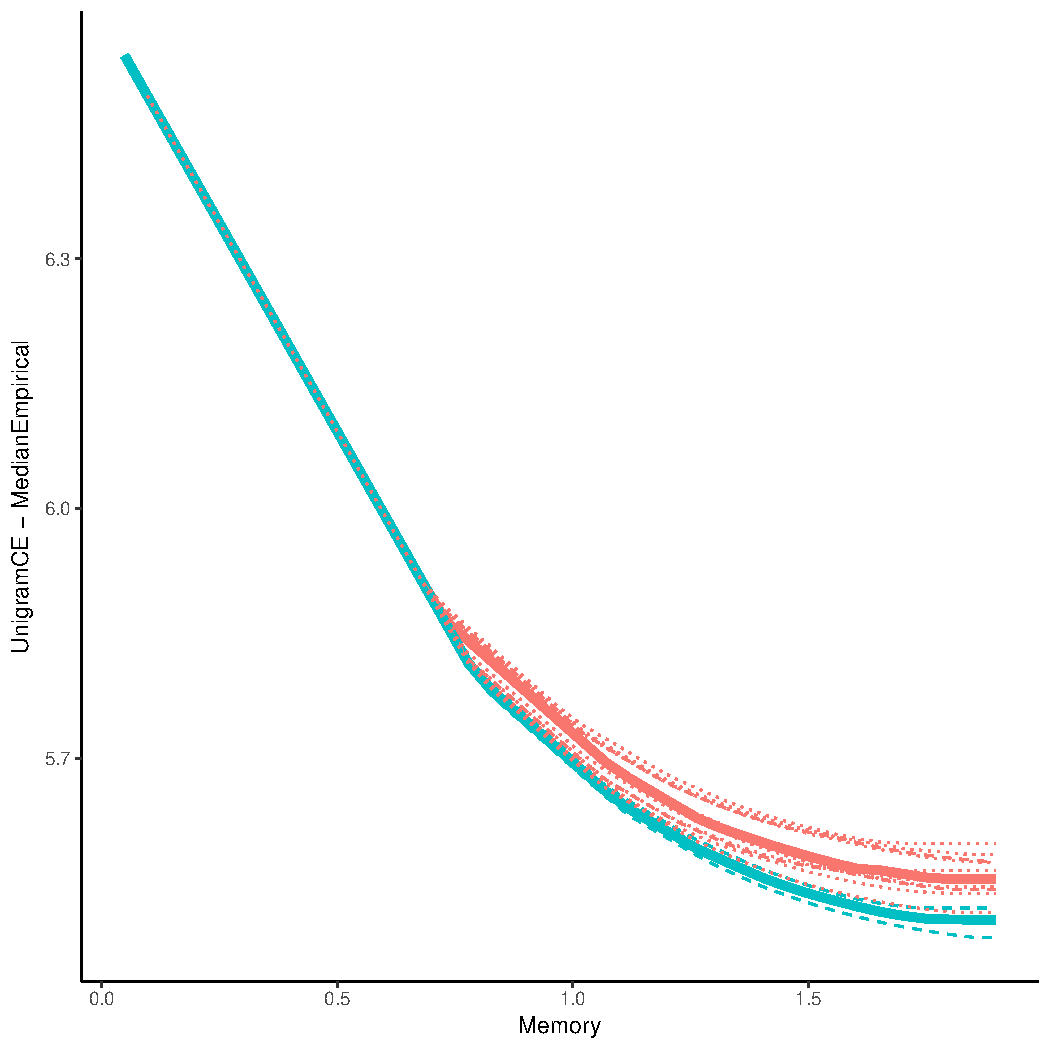
\includegraphics[width=0.25\textwidth]{neural/figures/German-listener-surprisal-memory-MEDIANS_QUANTILES_onlyWordForms_boundedVocab_REAL.pdf} & 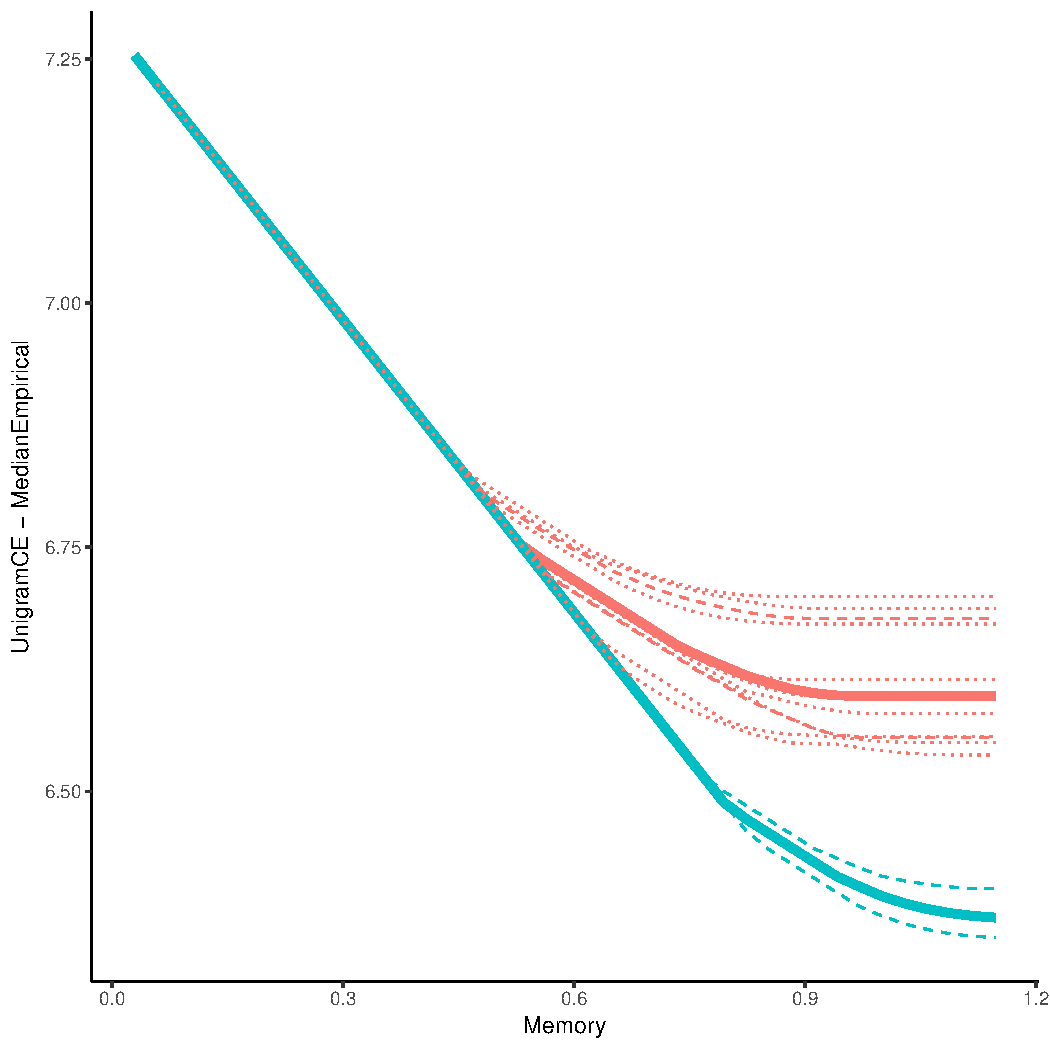
\includegraphics[width=0.25\textwidth]{neural/figures/Greek-listener-surprisal-memory-MEDIANS_QUANTILES_onlyWordForms_boundedVocab_REAL.pdf}
 \\ 
Hebrew & Hindi & Hungarian & Indonesian
 \\ 
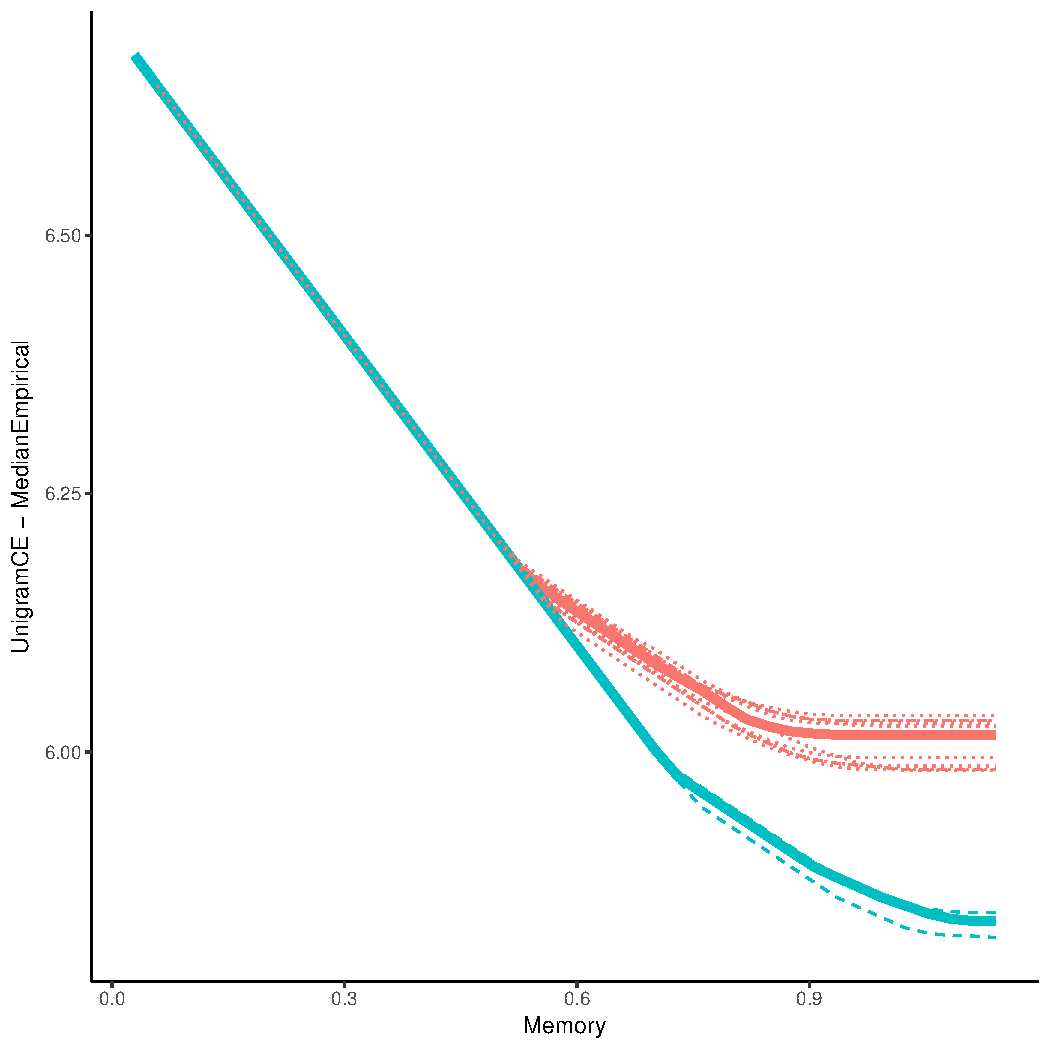
\includegraphics[width=0.25\textwidth]{neural/figures/Hebrew-listener-surprisal-memory-MEDIANS_QUANTILES_onlyWordForms_boundedVocab_REAL.pdf} & 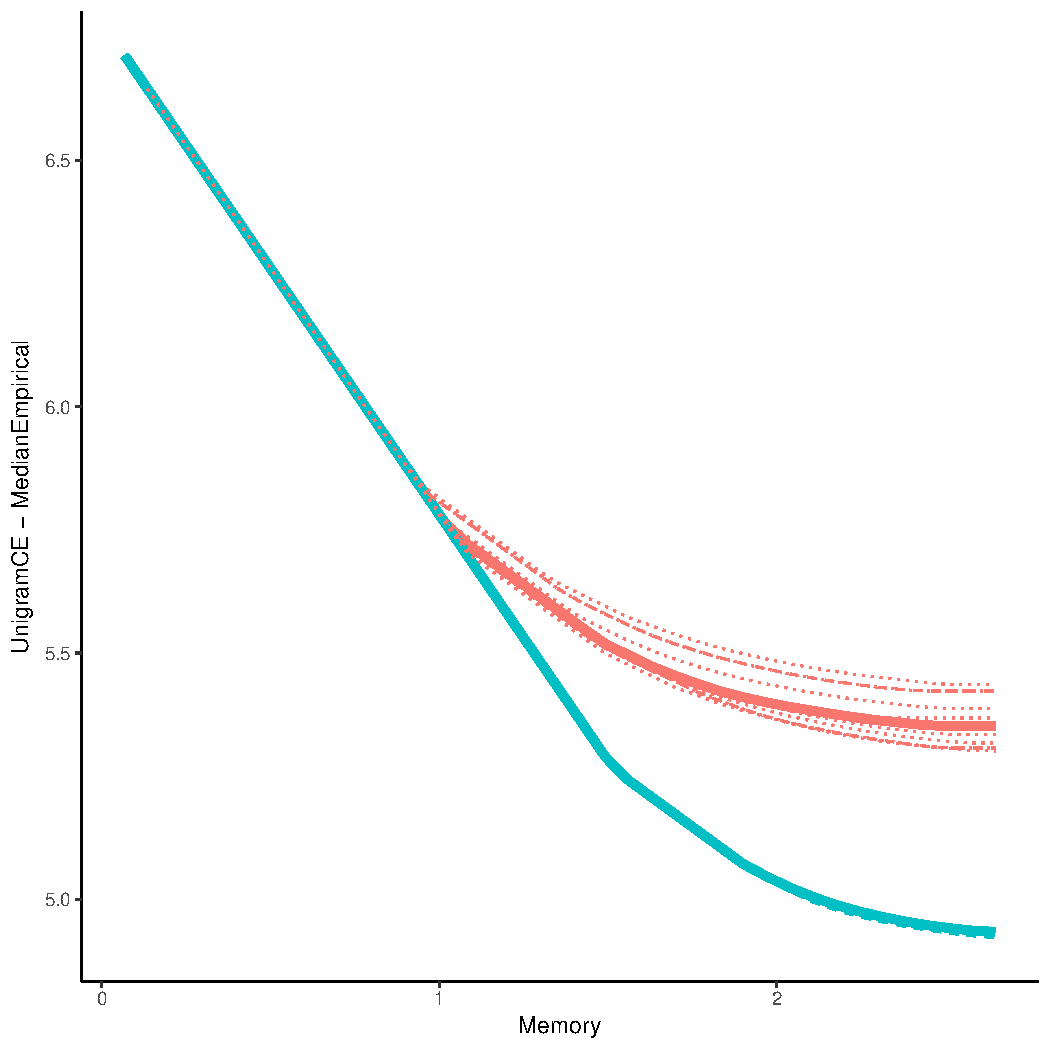
\includegraphics[width=0.25\textwidth]{neural/figures/Hindi-listener-surprisal-memory-MEDIANS_QUANTILES_onlyWordForms_boundedVocab_REAL.pdf} & 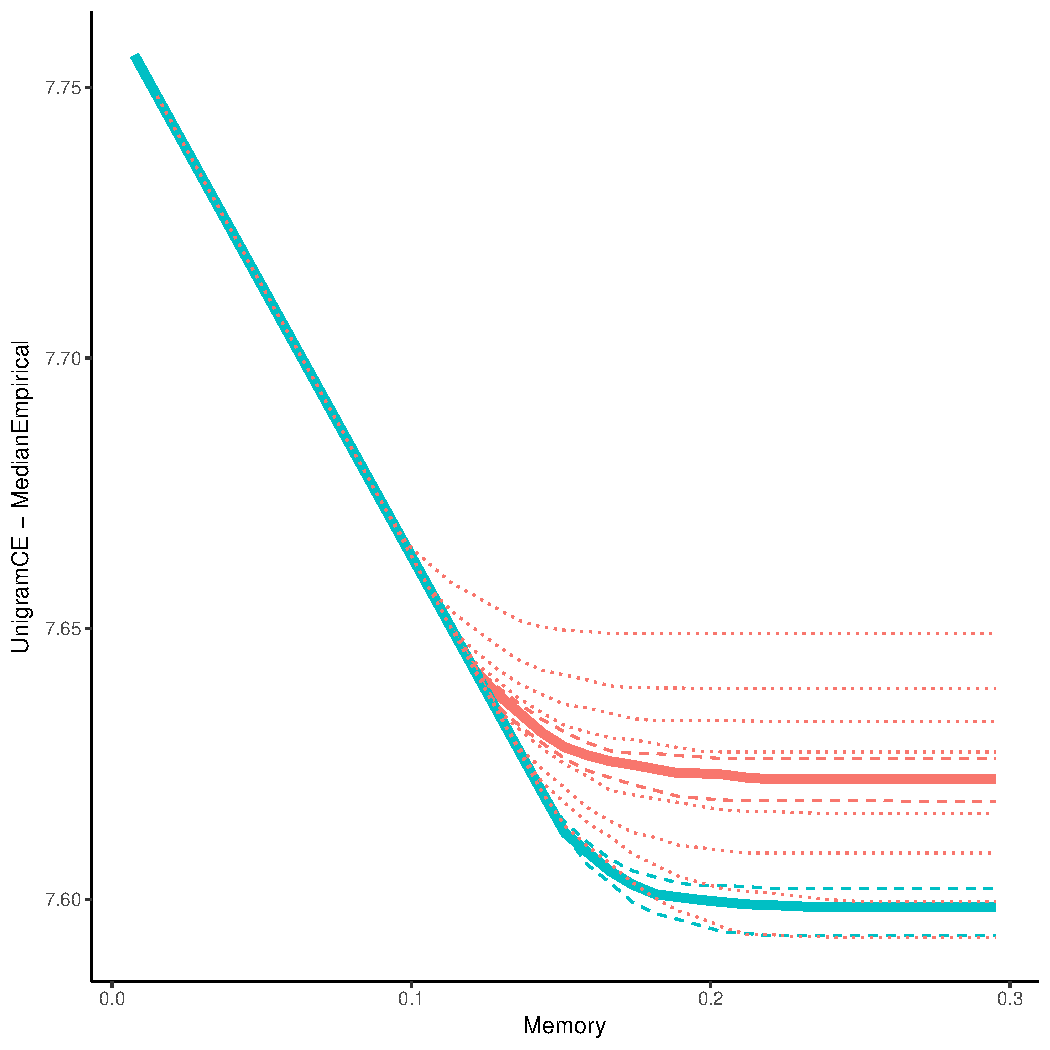
\includegraphics[width=0.25\textwidth]{neural/figures/Hungarian-listener-surprisal-memory-MEDIANS_QUANTILES_onlyWordForms_boundedVocab_REAL.pdf} & 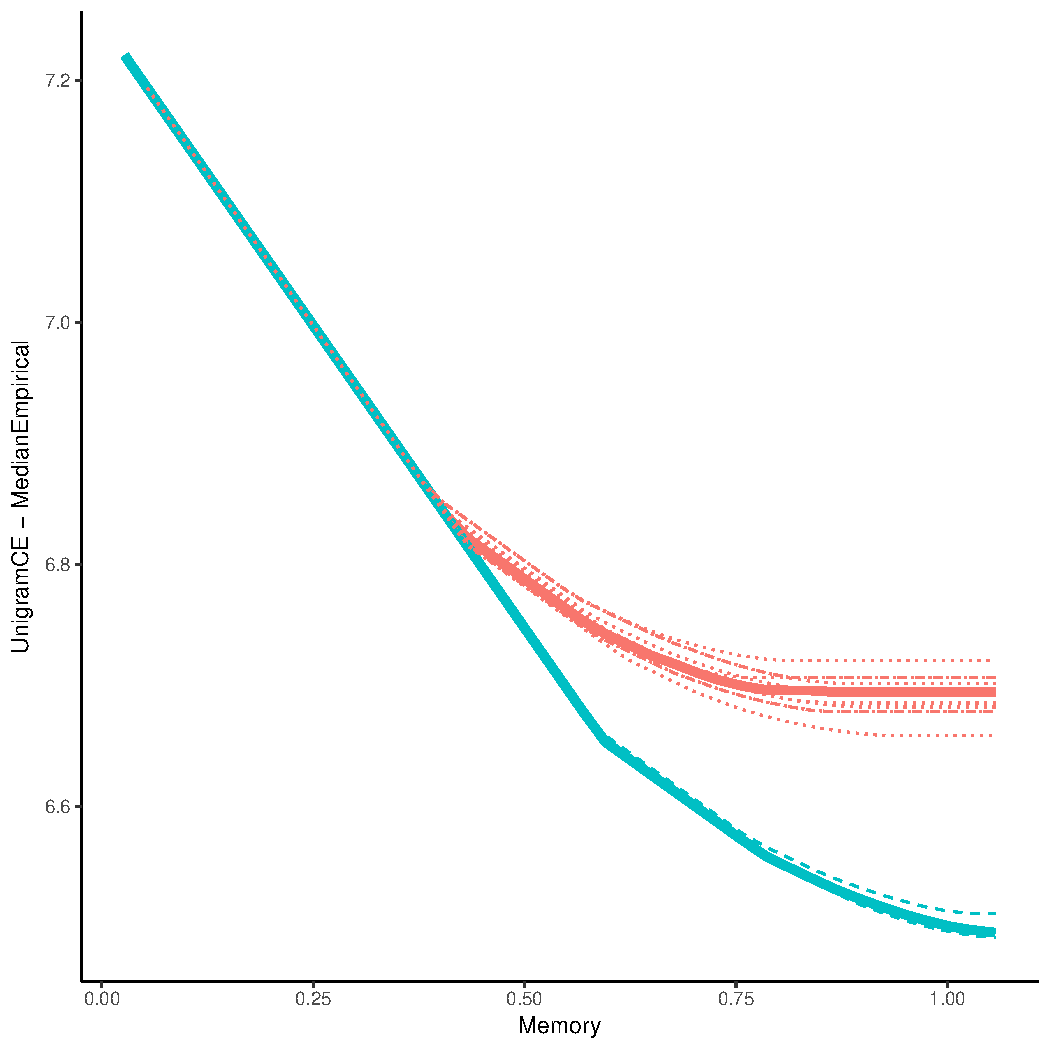
\includegraphics[width=0.25\textwidth]{neural/figures/Indonesian-listener-surprisal-memory-MEDIANS_QUANTILES_onlyWordForms_boundedVocab_REAL.pdf}
 \\ 
Italian & Japanese & Kazakh & Korean
 \\ 
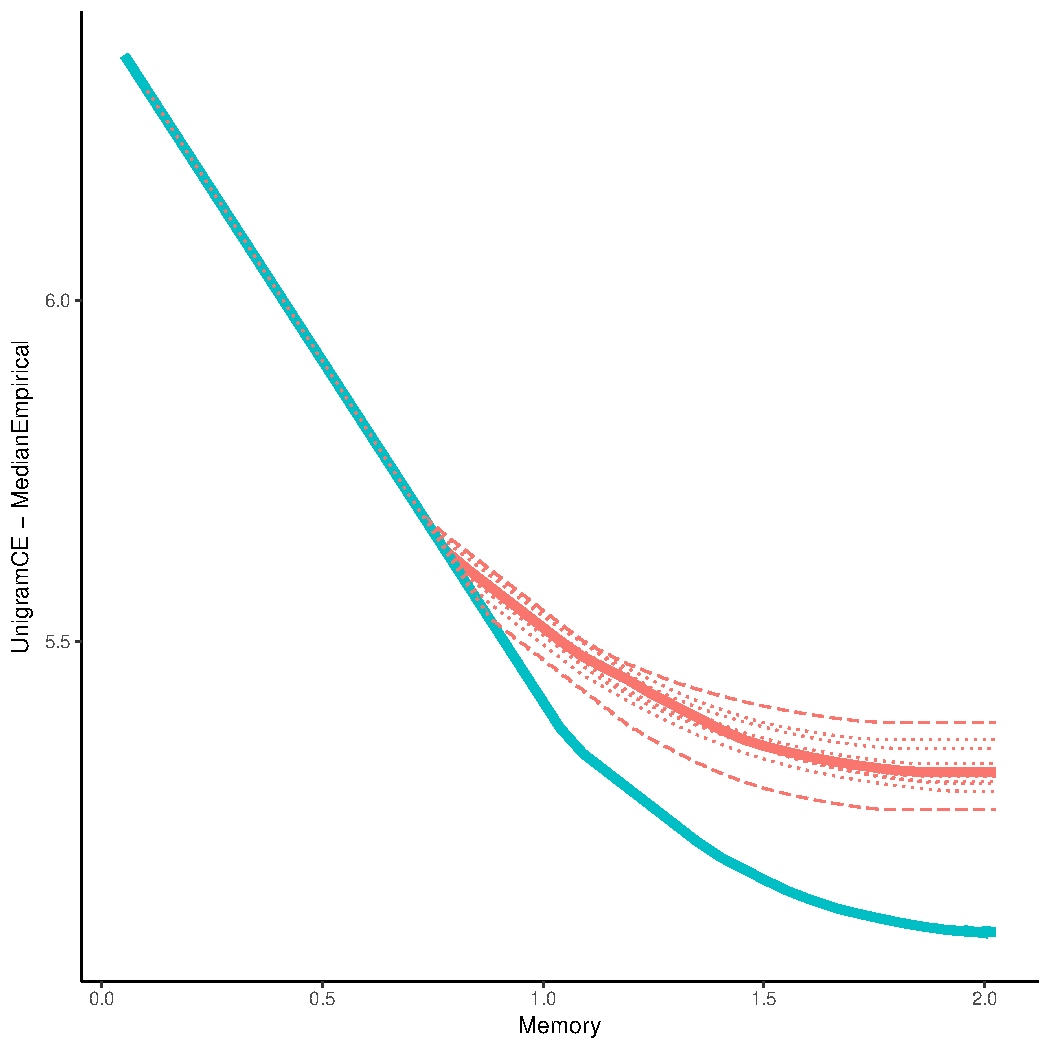
\includegraphics[width=0.25\textwidth]{neural/figures/Italian-listener-surprisal-memory-MEDIANS_QUANTILES_onlyWordForms_boundedVocab_REAL.pdf} & 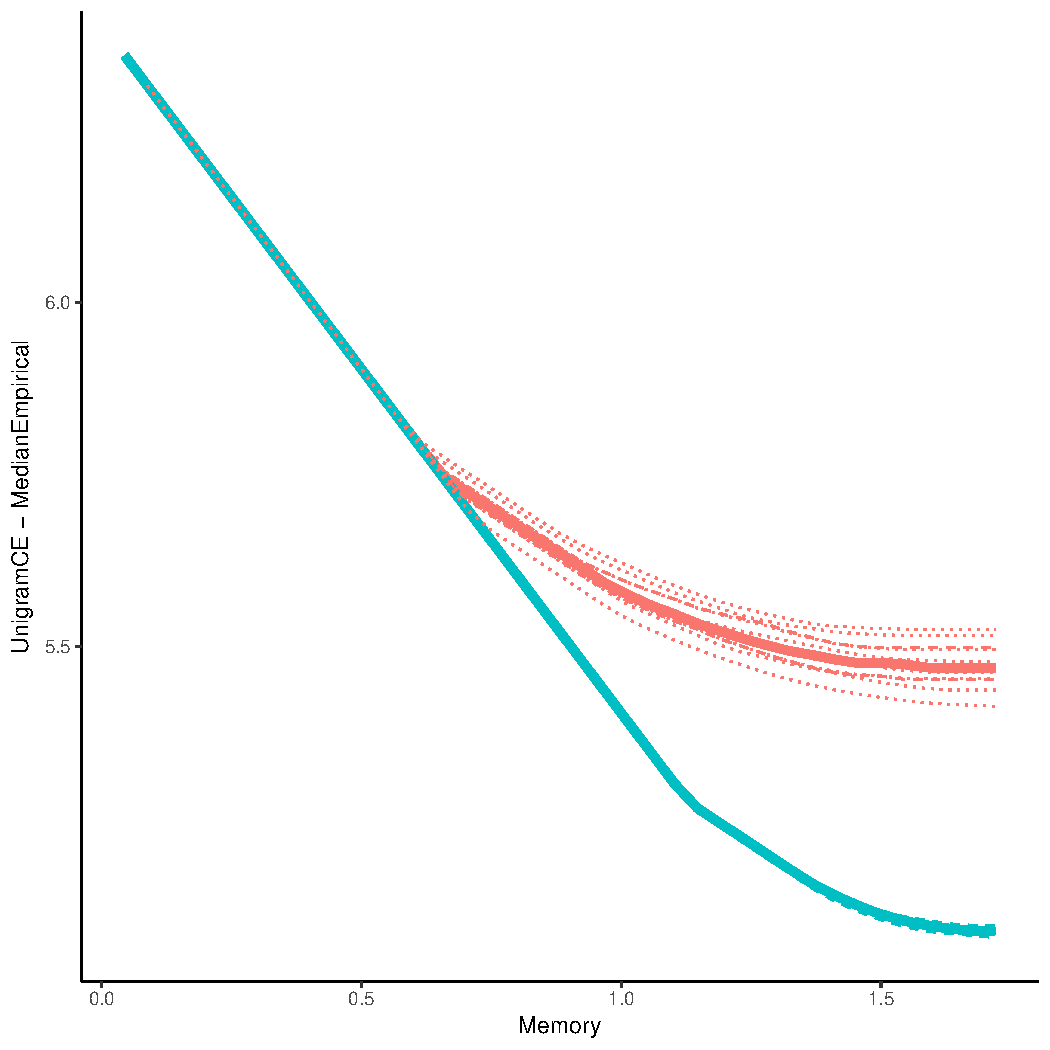
\includegraphics[width=0.25\textwidth]{neural/figures/Japanese-listener-surprisal-memory-MEDIANS_QUANTILES_onlyWordForms_boundedVocab_REAL.pdf} & 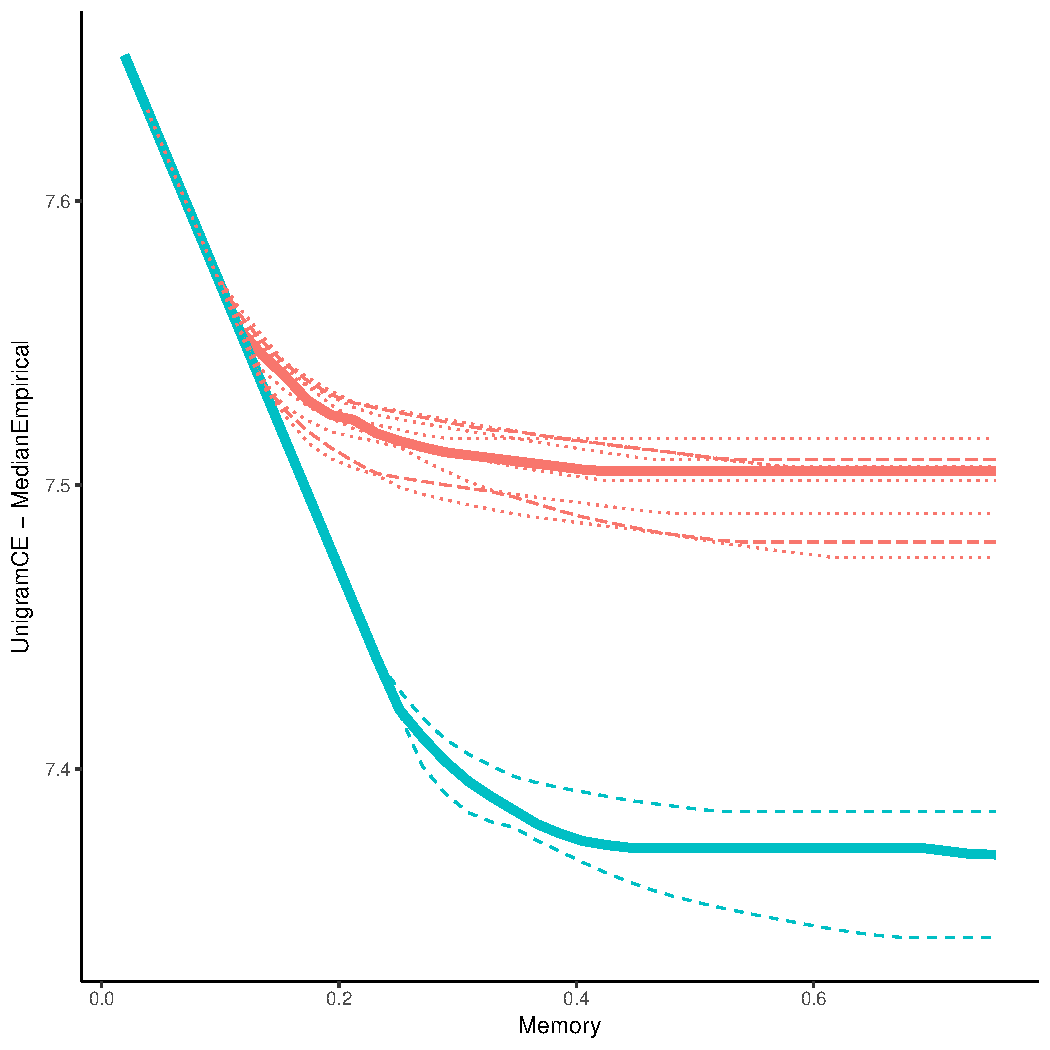
\includegraphics[width=0.25\textwidth]{neural/figures/Kazakh-Adap-listener-surprisal-memory-MEDIANS_QUANTILES_onlyWordForms_boundedVocab_REAL.pdf} & \includegraphics[width=0.25\textwidth]{neural/figures/Korean-listener-surprisal-memory-MEDIANS_QUANTILES_onlyWordForms_boundedVocab_REAL.pdf}
 \\ 

\end{longtable}
	\caption{Medians (cont.)}
\end{table}

\begin{table}[!htbp]
\begin{longtable}{ccccccccccccccclll}
Kurmanji & Latvian & Maltese & Naija
 \\ 
\includegraphics[width=0.25\textwidth]{neural/figures/Kurmanji-Adap-listener-surprisal-memory-MEDIANS_QUANTILES_onlyWordForms_boundedVocab_REAL.pdf} & \includegraphics[width=0.25\textwidth]{neural/figures/Latvian-listener-surprisal-memory-MEDIANS_QUANTILES_onlyWordForms_boundedVocab_REAL.pdf} & \includegraphics[width=0.25\textwidth]{neural/figures/Maltese-listener-surprisal-memory-MEDIANS_QUANTILES_onlyWordForms_boundedVocab_REAL.pdf} & \includegraphics[width=0.25\textwidth]{neural/figures/Naija-Adap-listener-surprisal-memory-MEDIANS_QUANTILES_onlyWordForms_boundedVocab_REAL.pdf}
 \\ 
North Sami & Norwegian & Persian & Polish
 \\ 
\includegraphics[width=0.25\textwidth]{neural/figures/North_Sami-listener-surprisal-memory-MEDIANS_QUANTILES_onlyWordForms_boundedVocab_REAL.pdf} & \includegraphics[width=0.25\textwidth]{neural/figures/Norwegian-listener-surprisal-memory-MEDIANS_QUANTILES_onlyWordForms_boundedVocab_REAL.pdf} & \includegraphics[width=0.25\textwidth]{neural/figures/Persian-listener-surprisal-memory-MEDIANS_QUANTILES_onlyWordForms_boundedVocab_REAL.pdf} & \includegraphics[width=0.25\textwidth]{neural/figures/Polish-listener-surprisal-memory-MEDIANS_QUANTILES_onlyWordForms_boundedVocab_REAL.pdf}
 \\ 
Portuguese & Romanian & Russian & Serbian
 \\ 
\includegraphics[width=0.25\textwidth]{neural/figures/Portuguese-listener-surprisal-memory-MEDIANS_QUANTILES_onlyWordForms_boundedVocab_REAL.pdf} & \includegraphics[width=0.25\textwidth]{neural/figures/Romanian-listener-surprisal-memory-MEDIANS_QUANTILES_onlyWordForms_boundedVocab_REAL.pdf} & \includegraphics[width=0.25\textwidth]{neural/figures/Russian-listener-surprisal-memory-MEDIANS_QUANTILES_onlyWordForms_boundedVocab_REAL.pdf} & \includegraphics[width=0.25\textwidth]{neural/figures/Serbian-listener-surprisal-memory-MEDIANS_QUANTILES_onlyWordForms_boundedVocab_REAL.pdf}
 \\ 
Slovak & Slovenian & Spanish & Swedish
 \\ 
\includegraphics[width=0.25\textwidth]{neural/figures/Slovak-listener-surprisal-memory-MEDIANS_QUANTILES_onlyWordForms_boundedVocab_REAL.pdf} & \includegraphics[width=0.25\textwidth]{neural/figures/Slovenian-listener-surprisal-memory-MEDIANS_QUANTILES_onlyWordForms_boundedVocab_REAL.pdf} & \includegraphics[width=0.25\textwidth]{neural/figures/Spanish-listener-surprisal-memory-MEDIANS_QUANTILES_onlyWordForms_boundedVocab_REAL.pdf} & \includegraphics[width=0.25\textwidth]{neural/figures/Swedish-listener-surprisal-memory-MEDIANS_QUANTILES_onlyWordForms_boundedVocab_REAL.pdf}
 \\ 

\end{longtable}
	\caption{Medians (cont.)}
\end{table}

\begin{table}[!htbp]
\begin{longtable}{ccccccccccccccclll}
Thai & Turkish & Ukrainian & Urdu
 \\ 
\includegraphics[width=0.25\textwidth]{neural/figures/Thai-Adap-listener-surprisal-memory-MEDIANS_onlyWordForms_boundedVocab_REAL.pdf} & \includegraphics[width=0.25\textwidth]{neural/figures/Turkish-listener-surprisal-memory-MEDIANS_onlyWordForms_boundedVocab_REAL.pdf} & \includegraphics[width=0.25\textwidth]{neural/figures/Ukrainian-listener-surprisal-memory-MEDIANS_onlyWordForms_boundedVocab_REAL.pdf} & \includegraphics[width=0.25\textwidth]{neural/figures/Urdu-listener-surprisal-memory-MEDIANS_onlyWordForms_boundedVocab_REAL.pdf}
 \\ 
Uyghur & Vietnamese &  & 
 \\ 
\includegraphics[width=0.25\textwidth]{neural/figures/Uyghur-Adap-listener-surprisal-memory-MEDIANS_onlyWordForms_boundedVocab_REAL.pdf} & \includegraphics[width=0.25\textwidth]{neural/figures/Vietnamese-listener-surprisal-memory-MEDIANS_onlyWordForms_boundedVocab_REAL.pdf} &  & 
 \\ 

\end{longtable}
	\caption{Medians (cont.)}
\end{table}







\begin{table}[!htbp]
\begin{tabular}{ccccccccccccccclll}
Afrikaans & Amharic & Arabic & Armenian
 \\ 
\includegraphics[width=0.25\textwidth]{neural/figures/Afrikaans-listener-surprisal-memory-HIST_byMem_onlyWordForms_boundedVocab_REAL.pdf} & \includegraphics[width=0.25\textwidth]{neural/figures/Amharic-Adap-listener-surprisal-memory-HIST_byMem_onlyWordForms_boundedVocab_REAL.pdf} & \includegraphics[width=0.25\textwidth]{neural/figures/Arabic-listener-surprisal-memory-HIST_byMem_onlyWordForms_boundedVocab_REAL.pdf} & \includegraphics[width=0.25\textwidth]{neural/figures/Armenian-Adap-listener-surprisal-memory-HIST_byMem_onlyWordForms_boundedVocab_REAL.pdf}
 \\ 
Bambara & Basque & Breton & Bulgarian
 \\ 
\includegraphics[width=0.25\textwidth]{neural/figures/Bambara-Adap-listener-surprisal-memory-HIST_byMem_onlyWordForms_boundedVocab_REAL.pdf} & \includegraphics[width=0.25\textwidth]{neural/figures/Basque-listener-surprisal-memory-HIST_byMem_onlyWordForms_boundedVocab_REAL.pdf} & \includegraphics[width=0.25\textwidth]{neural/figures/Breton-Adap-listener-surprisal-memory-HIST_byMem_onlyWordForms_boundedVocab_REAL.pdf} & \includegraphics[width=0.25\textwidth]{neural/figures/Bulgarian-listener-surprisal-memory-HIST_byMem_onlyWordForms_boundedVocab_REAL.pdf}
 \\ 
Buryat & Cantonese & Catalan & Chinese
 \\ 
\includegraphics[width=0.25\textwidth]{neural/figures/Buryat-Adap-listener-surprisal-memory-HIST_byMem_onlyWordForms_boundedVocab_REAL.pdf} & \includegraphics[width=0.25\textwidth]{neural/figures/Cantonese-Adap-listener-surprisal-memory-HIST_byMem_onlyWordForms_boundedVocab_REAL.pdf} & \includegraphics[width=0.25\textwidth]{neural/figures/Catalan-listener-surprisal-memory-HIST_byMem_onlyWordForms_boundedVocab_REAL.pdf} & \includegraphics[width=0.25\textwidth]{neural/figures/Chinese-listener-surprisal-memory-HIST_byMem_onlyWordForms_boundedVocab_REAL.pdf}
 \\ 
Croatian & Czech & Danish & Dutch
 \\ 
\includegraphics[width=0.25\textwidth]{neural/figures/Croatian-listener-surprisal-memory-HIST_byMem_onlyWordForms_boundedVocab_REAL.pdf} & \includegraphics[width=0.25\textwidth]{neural/figures/Czech-listener-surprisal-memory-HIST_byMem_onlyWordForms_boundedVocab_REAL.pdf} & \includegraphics[width=0.25\textwidth]{neural/figures/Danish-listener-surprisal-memory-HIST_byMem_onlyWordForms_boundedVocab_REAL.pdf} & \includegraphics[width=0.25\textwidth]{neural/figures/Dutch-listener-surprisal-memory-HIST_byMem_onlyWordForms_boundedVocab_REAL.pdf}
 \\ 

\end{tabular}
	\caption{Histograms: Surprisal, at maximum memory.}\label{tab:slice-hists-real}
\end{table}

\begin{table}[!htbp]
\begin{tabular}{ccccccccccccccclll}
English & Erzya & Estonian & Faroese
 \\ 
\includegraphics[width=0.25\textwidth]{neural/figures/English-listener-surprisal-memory-HIST_byMem_onlyWordForms_boundedVocab_REAL.pdf} & \includegraphics[width=0.25\textwidth]{neural/figures/Erzya-Adap-listener-surprisal-memory-HIST_byMem_onlyWordForms_boundedVocab_REAL.pdf} & \includegraphics[width=0.25\textwidth]{neural/figures/Estonian-listener-surprisal-memory-HIST_byMem_onlyWordForms_boundedVocab_REAL.pdf} & \includegraphics[width=0.25\textwidth]{neural/figures/Faroese-Adap-listener-surprisal-memory-HIST_byMem_onlyWordForms_boundedVocab_REAL.pdf}
 \\ 
Finnish & French & German & Greek
 \\ 
\includegraphics[width=0.25\textwidth]{neural/figures/Finnish-listener-surprisal-memory-HIST_byMem_onlyWordForms_boundedVocab_REAL.pdf} & \includegraphics[width=0.25\textwidth]{neural/figures/French-listener-surprisal-memory-HIST_byMem_onlyWordForms_boundedVocab_REAL.pdf} & \includegraphics[width=0.25\textwidth]{neural/figures/German-listener-surprisal-memory-HIST_byMem_onlyWordForms_boundedVocab_REAL.pdf} & \includegraphics[width=0.25\textwidth]{neural/figures/Greek-listener-surprisal-memory-HIST_byMem_onlyWordForms_boundedVocab_REAL.pdf}
 \\ 
Hebrew & Hindi & Hungarian & Indonesian
 \\ 
\includegraphics[width=0.25\textwidth]{neural/figures/Hebrew-listener-surprisal-memory-HIST_byMem_onlyWordForms_boundedVocab_REAL.pdf} & \includegraphics[width=0.25\textwidth]{neural/figures/Hindi-listener-surprisal-memory-HIST_byMem_onlyWordForms_boundedVocab_REAL.pdf} & \includegraphics[width=0.25\textwidth]{neural/figures/Hungarian-listener-surprisal-memory-HIST_byMem_onlyWordForms_boundedVocab_REAL.pdf} & \includegraphics[width=0.25\textwidth]{neural/figures/Indonesian-listener-surprisal-memory-HIST_byMem_onlyWordForms_boundedVocab_REAL.pdf}
 \\ 
Italian & Japanese & Kazakh & Korean
 \\ 
\includegraphics[width=0.25\textwidth]{neural/figures/Italian-listener-surprisal-memory-HIST_byMem_onlyWordForms_boundedVocab_REAL.pdf} & \includegraphics[width=0.25\textwidth]{neural/figures/Japanese-listener-surprisal-memory-HIST_byMem_onlyWordForms_boundedVocab_REAL.pdf} & \includegraphics[width=0.25\textwidth]{neural/figures/Kazakh-Adap-listener-surprisal-memory-HIST_byMem_onlyWordForms_boundedVocab_REAL.pdf} & \includegraphics[width=0.25\textwidth]{neural/figures/Korean-listener-surprisal-memory-HIST_byMem_onlyWordForms_boundedVocab_REAL.pdf}
 \\ 

\end{tabular}
	\caption{Medians (cont.)}
\end{table}

\begin{table}[!htbp]
\begin{tabular}{ccccccccccccccclll}
Kurmanji & Latvian & Maltese & Naija
 \\ 
\includegraphics[width=0.25\textwidth]{neural/figures/Kurmanji-Adap-listener-surprisal-memory-HIST_byMem_onlyWordForms_boundedVocab_REAL.pdf} & \includegraphics[width=0.25\textwidth]{neural/figures/Latvian-listener-surprisal-memory-HIST_byMem_onlyWordForms_boundedVocab_REAL.pdf} & \includegraphics[width=0.25\textwidth]{neural/figures/Maltese-listener-surprisal-memory-HIST_byMem_onlyWordForms_boundedVocab_REAL.pdf} & \includegraphics[width=0.25\textwidth]{neural/figures/Naija-Adap-listener-surprisal-memory-HIST_byMem_onlyWordForms_boundedVocab_REAL.pdf}
 \\ 
North Sami & Norwegian & Persian & Polish
 \\ 
\includegraphics[width=0.25\textwidth]{neural/figures/North_Sami-listener-surprisal-memory-HIST_byMem_onlyWordForms_boundedVocab_REAL.pdf} & \includegraphics[width=0.25\textwidth]{neural/figures/Norwegian-listener-surprisal-memory-HIST_byMem_onlyWordForms_boundedVocab_REAL.pdf} & \includegraphics[width=0.25\textwidth]{neural/figures/Persian-listener-surprisal-memory-HIST_byMem_onlyWordForms_boundedVocab_REAL.pdf} & \includegraphics[width=0.25\textwidth]{neural/figures/Polish-listener-surprisal-memory-HIST_byMem_onlyWordForms_boundedVocab_REAL.pdf}
 \\ 
Portuguese & Romanian & Russian & Serbian
 \\ 
\includegraphics[width=0.25\textwidth]{neural/figures/Portuguese-listener-surprisal-memory-HIST_byMem_onlyWordForms_boundedVocab_REAL.pdf} & \includegraphics[width=0.25\textwidth]{neural/figures/Romanian-listener-surprisal-memory-HIST_byMem_onlyWordForms_boundedVocab_REAL.pdf} & \includegraphics[width=0.25\textwidth]{neural/figures/Russian-listener-surprisal-memory-HIST_byMem_onlyWordForms_boundedVocab_REAL.pdf} & \includegraphics[width=0.25\textwidth]{neural/figures/Serbian-listener-surprisal-memory-HIST_byMem_onlyWordForms_boundedVocab_REAL.pdf}
 \\ 
Slovak & Slovenian & Spanish & Swedish
 \\ 
\includegraphics[width=0.25\textwidth]{neural/figures/Slovak-listener-surprisal-memory-HIST_byMem_onlyWordForms_boundedVocab_REAL.pdf} & \includegraphics[width=0.25\textwidth]{neural/figures/Slovenian-listener-surprisal-memory-HIST_byMem_onlyWordForms_boundedVocab_REAL.pdf} & \includegraphics[width=0.25\textwidth]{neural/figures/Spanish-listener-surprisal-memory-HIST_byMem_onlyWordForms_boundedVocab_REAL.pdf} & \includegraphics[width=0.25\textwidth]{neural/figures/Swedish-listener-surprisal-memory-HIST_byMem_onlyWordForms_boundedVocab_REAL.pdf}
 \\ 

\end{tabular}
	\caption{Medians (cont.)}
\end{table}

\begin{table}[!htbp]
\begin{tabular}{ccccccccccccccclll}
Thai & Turkish & Ukrainian & Urdu
 \\ 
\includegraphics[width=0.25\textwidth]{neural/figures/Thai-Adap-listener-surprisal-memory-HIST_byMem_onlyWordForms_boundedVocab_REAL.pdf} & \includegraphics[width=0.25\textwidth]{neural/figures/Turkish-listener-surprisal-memory-HIST_byMem_onlyWordForms_boundedVocab_REAL.pdf} & \includegraphics[width=0.25\textwidth]{neural/figures/Ukrainian-listener-surprisal-memory-HIST_byMem_onlyWordForms_boundedVocab_REAL.pdf} & \includegraphics[width=0.25\textwidth]{neural/figures/Urdu-listener-surprisal-memory-HIST_byMem_onlyWordForms_boundedVocab_REAL.pdf}
 \\ 
Uyghur & Vietnamese &  & 
 \\ 
\includegraphics[width=0.25\textwidth]{neural/figures/Uyghur-Adap-listener-surprisal-memory-HIST_byMem_onlyWordForms_boundedVocab_REAL.pdf} & \includegraphics[width=0.25\textwidth]{neural/figures/Vietnamese-listener-surprisal-memory-HIST_byMem_onlyWordForms_boundedVocab_REAL.pdf} &  & 
 \\ 

\end{tabular}
	\caption{Medians (cont.)}
\end{table}


%\begin{table}
%\begin{tabular}{cccccccccccccccccc}
%Afrikaans & Amharic & Arabic & Armenian
 \\ 
\includegraphics[width=0.25\textwidth]{neural/figures/Afrikaans-listener-surprisal-memory-QUANTILES_onlyWordForms_boundedVocab_REAL.pdf} & \includegraphics[width=0.25\textwidth]{neural/figures/Amharic-Adap-listener-surprisal-memory-QUANTILES_onlyWordForms_boundedVocab_REAL.pdf} & \includegraphics[width=0.25\textwidth]{neural/figures/Arabic-listener-surprisal-memory-QUANTILES_onlyWordForms_boundedVocab_REAL.pdf} & \includegraphics[width=0.25\textwidth]{neural/figures/Armenian-Adap-listener-surprisal-memory-QUANTILES_onlyWordForms_boundedVocab_REAL.pdf}
 \\ 
Bambara & Basque & Breton & Bulgarian
 \\ 
\includegraphics[width=0.25\textwidth]{neural/figures/Bambara-Adap-listener-surprisal-memory-QUANTILES_onlyWordForms_boundedVocab_REAL.pdf} & \includegraphics[width=0.25\textwidth]{neural/figures/Basque-listener-surprisal-memory-QUANTILES_onlyWordForms_boundedVocab_REAL.pdf} & \includegraphics[width=0.25\textwidth]{neural/figures/Breton-Adap-listener-surprisal-memory-QUANTILES_onlyWordForms_boundedVocab_REAL.pdf} & \includegraphics[width=0.25\textwidth]{neural/figures/Bulgarian-listener-surprisal-memory-QUANTILES_onlyWordForms_boundedVocab_REAL.pdf}
 \\ 
Buryat & Cantonese & Catalan & Chinese
 \\ 
\includegraphics[width=0.25\textwidth]{neural/figures/Buryat-Adap-listener-surprisal-memory-QUANTILES_onlyWordForms_boundedVocab_REAL.pdf} & \includegraphics[width=0.25\textwidth]{neural/figures/Cantonese-Adap-listener-surprisal-memory-QUANTILES_onlyWordForms_boundedVocab_REAL.pdf} & \includegraphics[width=0.25\textwidth]{neural/figures/Catalan-listener-surprisal-memory-QUANTILES_onlyWordForms_boundedVocab_REAL.pdf} & \includegraphics[width=0.25\textwidth]{neural/figures/Chinese-listener-surprisal-memory-QUANTILES_onlyWordForms_boundedVocab_REAL.pdf}
 \\ 
Croatian & Czech & Danish & Dutch
 \\ 
\includegraphics[width=0.25\textwidth]{neural/figures/Croatian-listener-surprisal-memory-QUANTILES_onlyWordForms_boundedVocab_REAL.pdf} & \includegraphics[width=0.25\textwidth]{neural/figures/Czech-listener-surprisal-memory-QUANTILES_onlyWordForms_boundedVocab_REAL.pdf} & \includegraphics[width=0.25\textwidth]{neural/figures/Danish-listener-surprisal-memory-QUANTILES_onlyWordForms_boundedVocab_REAL.pdf} & \includegraphics[width=0.25\textwidth]{neural/figures/Dutch-listener-surprisal-memory-QUANTILES_onlyWordForms_boundedVocab_REAL.pdf}
 \\ 
English & Erzya & Estonian & Faroese
 \\ 
\includegraphics[width=0.25\textwidth]{neural/figures/English-listener-surprisal-memory-QUANTILES_onlyWordForms_boundedVocab_REAL.pdf} & \includegraphics[width=0.25\textwidth]{neural/figures/Erzya-Adap-listener-surprisal-memory-QUANTILES_onlyWordForms_boundedVocab_REAL.pdf} & \includegraphics[width=0.25\textwidth]{neural/figures/Estonian-listener-surprisal-memory-QUANTILES_onlyWordForms_boundedVocab_REAL.pdf} & \includegraphics[width=0.25\textwidth]{neural/figures/Faroese-Adap-listener-surprisal-memory-QUANTILES_onlyWordForms_boundedVocab_REAL.pdf}
 \\ 

%\end{tabular}
%	\caption{Quantiles: At a given memory budget, what percentage of the baselines results in higher listener surprisal than the real language? Solid curves represent sample means, dashed lines represent 95 \% confidence bounds; dotted lines represent 99.9 \% confidence bounds. At five evenly spaced memory levels, we provide a p-value for the null hypothesis that the actual population mean is $0.5$ or less. Confidence bounds and p-values are obtained using an exact nonparametric method (see text).}\label{tab:quantiles}
%\end{table}
%
%\begin{table}
%\begin{tabular}{cccccccccccccccccc}
%Finnish & French & German & Greek
 \\ 
\includegraphics[width=0.25\textwidth]{neural/figures/Finnish-listener-surprisal-memory-QUANTILES_onlyWordForms_boundedVocab_REAL.pdf} & \includegraphics[width=0.25\textwidth]{neural/figures/French-listener-surprisal-memory-QUANTILES_onlyWordForms_boundedVocab_REAL.pdf} & \includegraphics[width=0.25\textwidth]{neural/figures/German-listener-surprisal-memory-QUANTILES_onlyWordForms_boundedVocab_REAL.pdf} & \includegraphics[width=0.25\textwidth]{neural/figures/Greek-listener-surprisal-memory-QUANTILES_onlyWordForms_boundedVocab_REAL.pdf}
 \\ 
Hebrew & Hindi & Hungarian & Indonesian
 \\ 
\includegraphics[width=0.25\textwidth]{neural/figures/Hebrew-listener-surprisal-memory-QUANTILES_onlyWordForms_boundedVocab_REAL.pdf} & \includegraphics[width=0.25\textwidth]{neural/figures/Hindi-listener-surprisal-memory-QUANTILES_onlyWordForms_boundedVocab_REAL.pdf} & \includegraphics[width=0.25\textwidth]{neural/figures/Hungarian-listener-surprisal-memory-QUANTILES_onlyWordForms_boundedVocab_REAL.pdf} & \includegraphics[width=0.25\textwidth]{neural/figures/Indonesian-listener-surprisal-memory-QUANTILES_onlyWordForms_boundedVocab_REAL.pdf}
 \\ 
Italian & Japanese & Kazakh & Korean
 \\ 
\includegraphics[width=0.25\textwidth]{neural/figures/Italian-listener-surprisal-memory-QUANTILES_onlyWordForms_boundedVocab_REAL.pdf} & \includegraphics[width=0.25\textwidth]{neural/figures/Japanese-listener-surprisal-memory-QUANTILES_onlyWordForms_boundedVocab_REAL.pdf} & \includegraphics[width=0.25\textwidth]{neural/figures/Kazakh-Adap-listener-surprisal-memory-QUANTILES_onlyWordForms_boundedVocab_REAL.pdf} & \includegraphics[width=0.25\textwidth]{neural/figures/Korean-listener-surprisal-memory-QUANTILES_onlyWordForms_boundedVocab_REAL.pdf}
 \\ 
Kurmanji & Latvian & Maltese & Naija
 \\ 
\includegraphics[width=0.25\textwidth]{neural/figures/Kurmanji-Adap-listener-surprisal-memory-QUANTILES_onlyWordForms_boundedVocab_REAL.pdf} & \includegraphics[width=0.25\textwidth]{neural/figures/Latvian-listener-surprisal-memory-QUANTILES_onlyWordForms_boundedVocab_REAL.pdf} & \includegraphics[width=0.25\textwidth]{neural/figures/Maltese-listener-surprisal-memory-QUANTILES_onlyWordForms_boundedVocab_REAL.pdf} & \includegraphics[width=0.25\textwidth]{neural/figures/Naija-Adap-listener-surprisal-memory-QUANTILES_onlyWordForms_boundedVocab_REAL.pdf}
 \\ 
North Sami & Norwegian & Persian & Polish
 \\ 
\includegraphics[width=0.25\textwidth]{neural/figures/North_Sami-listener-surprisal-memory-QUANTILES_onlyWordForms_boundedVocab_REAL.pdf} & \includegraphics[width=0.25\textwidth]{neural/figures/Norwegian-listener-surprisal-memory-QUANTILES_onlyWordForms_boundedVocab_REAL.pdf} & \includegraphics[width=0.25\textwidth]{neural/figures/Persian-listener-surprisal-memory-QUANTILES_onlyWordForms_boundedVocab_REAL.pdf} & \includegraphics[width=0.25\textwidth]{neural/figures/Polish-listener-surprisal-memory-QUANTILES_onlyWordForms_boundedVocab_REAL.pdf}
 \\ 

%\end{tabular}
%	\caption{Quantiles (part 2)}
%\end{table}
%
%\begin{table}
%\begin{tabular}{cccccccccccccccccc}
%Portuguese & Romanian & Russian & Serbian
 \\ 
\includegraphics[width=0.25\textwidth]{neural/figures/Portuguese-listener-surprisal-memory-QUANTILES_onlyWordForms_boundedVocab_REAL.pdf} & \includegraphics[width=0.25\textwidth]{neural/figures/Romanian-listener-surprisal-memory-QUANTILES_onlyWordForms_boundedVocab_REAL.pdf} & \includegraphics[width=0.25\textwidth]{neural/figures/Russian-listener-surprisal-memory-QUANTILES_onlyWordForms_boundedVocab_REAL.pdf} & \includegraphics[width=0.25\textwidth]{neural/figures/Serbian-listener-surprisal-memory-QUANTILES_onlyWordForms_boundedVocab_REAL.pdf}
 \\ 
Slovak & Slovenian & Spanish & Swedish
 \\ 
\includegraphics[width=0.25\textwidth]{neural/figures/Slovak-listener-surprisal-memory-QUANTILES_onlyWordForms_boundedVocab_REAL.pdf} & \includegraphics[width=0.25\textwidth]{neural/figures/Slovenian-listener-surprisal-memory-QUANTILES_onlyWordForms_boundedVocab_REAL.pdf} & \includegraphics[width=0.25\textwidth]{neural/figures/Spanish-listener-surprisal-memory-QUANTILES_onlyWordForms_boundedVocab_REAL.pdf} & \includegraphics[width=0.25\textwidth]{neural/figures/Swedish-listener-surprisal-memory-QUANTILES_onlyWordForms_boundedVocab_REAL.pdf}
 \\ 
Thai & Turkish & Ukrainian & Urdu
 \\ 
\includegraphics[width=0.25\textwidth]{neural/figures/Thai-Adap-listener-surprisal-memory-QUANTILES_onlyWordForms_boundedVocab_REAL.pdf} & \includegraphics[width=0.25\textwidth]{neural/figures/Turkish-listener-surprisal-memory-QUANTILES_onlyWordForms_boundedVocab_REAL.pdf} & \includegraphics[width=0.25\textwidth]{neural/figures/Ukrainian-listener-surprisal-memory-QUANTILES_onlyWordForms_boundedVocab_REAL.pdf} & \includegraphics[width=0.25\textwidth]{neural/figures/Urdu-listener-surprisal-memory-QUANTILES_onlyWordForms_boundedVocab_REAL.pdf}
 \\ 
Uyghur & Vietnamese &  & 
 \\ 
\includegraphics[width=0.25\textwidth]{neural/figures/Uyghur-Adap-listener-surprisal-memory-QUANTILES_onlyWordForms_boundedVocab_REAL.pdf} & \includegraphics[width=0.25\textwidth]{neural/figures/Vietnamese-listener-surprisal-memory-QUANTILES_onlyWordForms_boundedVocab_REAL.pdf} &  & 
 \\ 

%\end{tabular}
%	\caption{Quantiles (part 3)}
%\end{table}
%
%
%


















\begin{table}[!htbp]
\begin{tabular}{l|ll||l|llllllllllllll}
	Language & Base. & MLE & Language & Base. & MLE \\ \hline
Afrikaans  &  13  &  10  &  Indonesian  &  11  &  10  \\
Amharic  &  137  &  71  &  Italian  &  10  &  10  \\
Arabic  &  11  &  10  &  Japanese  &  25  &  10  \\
Armenian  &  140  &  17  &  Kazakh  &  11  &  10  \\
Bambara  &  25  &  10  &  Korean  &  11  &  10  \\
Basque  &  15  &  10  &  Kurmanji  &  338  &  101  \\
Breton  &  35  &  10  &  Latvian  &  308  &  132  \\
Bulgarian  &  14  &  10  &  Maltese  &  30  &  10  \\
Buryat  &  26  &  10  &  Naija  &  214  &  93  \\
Cantonese  &  306  &  135  &  North Sami  &  335  &  101  \\
Catalan  &  11  &  10  &  Norwegian  &  12  &  10  \\
Chinese  &  21  &  10  &  Persian  &  25  &  10  \\
Croatian  &  30  &  10  &  Polish  &  309  &  131  \\
Czech  &  18  &  12  &  Portuguese  &  15  &  99  \\
Danish  &  33  &  10  &  Romanian  &  10  &  10  \\
Dutch  &  27  &  10  &  Russian  &  20  &  13  \\
English  &  13  &  10  &  Serbian  &  26  &  11  \\
Erzya  &  846  &  101  &  Slovak  &  303  &  138  \\
Estonian  &  347  &  10  &  Slovenian  &  297  &  12  \\
Faroese  &  27  &  10  &  Spanish  &  14  &  10  \\
Finnish  &  83  &  54  &  Swedish  &  31  &  10  \\
French  &  14  &  12  &  Thai  &  45  &  10  \\
German  &  19  &  10  &  Turkish  &  13  &  10  \\
Greek  &  16  &  10  &  Ukrainian  &  28  &  10  \\
Hebrew  &  11  &  10  &  Urdu  &  17  &  10  \\
Hindi  &  11  &  10  &  Uyghur  &  326  &  132  \\
Hungarian  &  220  &  35  &  Vietnamese  &  303  &  132  \\

\end{tabular}
	\caption{Experiment 3: Samples drawn per language according to the precision-dependent stopping criterion.}\label{tab:samples}
\end{table}





\begin{table}[!htbp]
\begin{tabular}{ccccccccccccccclll}
Afrikaans & Amharic & Arabic & Armenian
 \\ 
\includegraphics[width=0.25\textwidth]{neural/figures/Afrikaans-listener-surprisal-memory-MEDIANS_QUANTILES_onlyWordForms_boundedVocab.pdf} & \includegraphics[width=0.25\textwidth]{neural/figures/Amharic-Adap-listener-surprisal-memory-MEDIANS_QUANTILES_onlyWordForms_boundedVocab.pdf} & \includegraphics[width=0.25\textwidth]{neural/figures/Arabic-listener-surprisal-memory-MEDIANS_QUANTILES_onlyWordForms_boundedVocab.pdf} & \includegraphics[width=0.25\textwidth]{neural/figures/Armenian-Adap-listener-surprisal-memory-MEDIANS_QUANTILES_onlyWordForms_boundedVocab.pdf}
 \\ 
Bambara & Basque & Breton & Bulgarian
 \\ 
\includegraphics[width=0.25\textwidth]{neural/figures/Bambara-Adap-listener-surprisal-memory-MEDIANS_QUANTILES_onlyWordForms_boundedVocab.pdf} & \includegraphics[width=0.25\textwidth]{neural/figures/Basque-listener-surprisal-memory-MEDIANS_QUANTILES_onlyWordForms_boundedVocab.pdf} & \includegraphics[width=0.25\textwidth]{neural/figures/Breton-Adap-listener-surprisal-memory-MEDIANS_QUANTILES_onlyWordForms_boundedVocab.pdf} & \includegraphics[width=0.25\textwidth]{neural/figures/Bulgarian-listener-surprisal-memory-MEDIANS_QUANTILES_onlyWordForms_boundedVocab.pdf}
 \\ 
Buryat & Cantonese & Catalan & Chinese
 \\ 
\includegraphics[width=0.25\textwidth]{neural/figures/Buryat-Adap-listener-surprisal-memory-MEDIANS_QUANTILES_onlyWordForms_boundedVocab.pdf} & \includegraphics[width=0.25\textwidth]{neural/figures/Cantonese-Adap-listener-surprisal-memory-MEDIANS_QUANTILES_onlyWordForms_boundedVocab.pdf} & \includegraphics[width=0.25\textwidth]{neural/figures/Catalan-listener-surprisal-memory-MEDIANS_QUANTILES_onlyWordForms_boundedVocab.pdf} & \includegraphics[width=0.25\textwidth]{neural/figures/Chinese-listener-surprisal-memory-MEDIANS_QUANTILES_onlyWordForms_boundedVocab.pdf}
 \\ 
Croatian & Czech & Danish & Dutch
 \\ 
\includegraphics[width=0.25\textwidth]{neural/figures/Croatian-listener-surprisal-memory-MEDIANS_QUANTILES_onlyWordForms_boundedVocab.pdf} & \includegraphics[width=0.25\textwidth]{neural/figures/Czech-listener-surprisal-memory-MEDIANS_QUANTILES_onlyWordForms_boundedVocab.pdf} & \includegraphics[width=0.25\textwidth]{neural/figures/Danish-listener-surprisal-memory-MEDIANS_QUANTILES_onlyWordForms_boundedVocab.pdf} & \includegraphics[width=0.25\textwidth]{neural/figures/Dutch-listener-surprisal-memory-MEDIANS_QUANTILES_onlyWordForms_boundedVocab.pdf}
 \\ 

\end{tabular}
	\caption{Experiment 3. Medians: For each memory budget, we provide the median surprisal for real and random languages. Solid lines indicate sample medians, dashed lines indicate 95 $\%$ confidence intervals for the population median. Green: Random baselines; blue: real language; red: maximum-likelihood grammars fit to real orderings.}\label{tab:medians}
\end{table}

\begin{table}[!htbp]
\begin{tabular}{ccccccccccccccclll}
English & Erzya & Estonian & Faroese
 \\ 
\includegraphics[width=0.25\textwidth]{neural/figures/English-listener-surprisal-memory-MEDIANS_onlyWordForms_boundedVocab.pdf} & \includegraphics[width=0.25\textwidth]{neural/figures/Erzya-Adap-listener-surprisal-memory-MEDIANS_onlyWordForms_boundedVocab.pdf} & \includegraphics[width=0.25\textwidth]{neural/figures/Estonian-listener-surprisal-memory-MEDIANS_onlyWordForms_boundedVocab.pdf} & \includegraphics[width=0.25\textwidth]{neural/figures/Faroese-Adap-listener-surprisal-memory-MEDIANS_onlyWordForms_boundedVocab.pdf}
 \\ 
Finnish & French & German & Greek
 \\ 
\includegraphics[width=0.25\textwidth]{neural/figures/Finnish-listener-surprisal-memory-MEDIANS_onlyWordForms_boundedVocab.pdf} & \includegraphics[width=0.25\textwidth]{neural/figures/French-listener-surprisal-memory-MEDIANS_onlyWordForms_boundedVocab.pdf} & \includegraphics[width=0.25\textwidth]{neural/figures/German-listener-surprisal-memory-MEDIANS_onlyWordForms_boundedVocab.pdf} & \includegraphics[width=0.25\textwidth]{neural/figures/Greek-listener-surprisal-memory-MEDIANS_onlyWordForms_boundedVocab.pdf}
 \\ 
Hebrew & Hindi & Hungarian & Indonesian
 \\ 
\includegraphics[width=0.25\textwidth]{neural/figures/Hebrew-listener-surprisal-memory-MEDIANS_onlyWordForms_boundedVocab.pdf} & \includegraphics[width=0.25\textwidth]{neural/figures/Hindi-listener-surprisal-memory-MEDIANS_onlyWordForms_boundedVocab.pdf} & \includegraphics[width=0.25\textwidth]{neural/figures/Hungarian-listener-surprisal-memory-MEDIANS_onlyWordForms_boundedVocab.pdf} & \includegraphics[width=0.25\textwidth]{neural/figures/Indonesian-listener-surprisal-memory-MEDIANS_onlyWordForms_boundedVocab.pdf}
 \\ 
Italian & Japanese & Kazakh & Korean
 \\ 
\includegraphics[width=0.25\textwidth]{neural/figures/Italian-listener-surprisal-memory-MEDIANS_onlyWordForms_boundedVocab.pdf} & \includegraphics[width=0.25\textwidth]{neural/figures/Japanese-listener-surprisal-memory-MEDIANS_onlyWordForms_boundedVocab.pdf} & \includegraphics[width=0.25\textwidth]{neural/figures/Kazakh-Adap-listener-surprisal-memory-MEDIANS_onlyWordForms_boundedVocab.pdf} & \includegraphics[width=0.25\textwidth]{neural/figures/Korean-listener-surprisal-memory-MEDIANS_onlyWordForms_boundedVocab.pdf}
 \\ 

\end{tabular}
	\caption{Medians (cont.)}
\end{table}

\begin{table}[!htbp]
\begin{tabular}{ccccccccccccccclll}
Kurmanji & Latvian & Maltese & Naija
 \\ 
\includegraphics[width=0.25\textwidth]{neural/figures/Kurmanji-Adap-listener-surprisal-memory-MEDIANS_onlyWordForms_boundedVocab.pdf} & \includegraphics[width=0.25\textwidth]{neural/figures/Latvian-listener-surprisal-memory-MEDIANS_onlyWordForms_boundedVocab.pdf} & \includegraphics[width=0.25\textwidth]{neural/figures/Maltese-listener-surprisal-memory-MEDIANS_onlyWordForms_boundedVocab.pdf} & \includegraphics[width=0.25\textwidth]{neural/figures/Naija-Adap-listener-surprisal-memory-MEDIANS_onlyWordForms_boundedVocab.pdf}
 \\ 
North Sami & Norwegian & Persian & Polish
 \\ 
\includegraphics[width=0.25\textwidth]{neural/figures/North_Sami-listener-surprisal-memory-MEDIANS_onlyWordForms_boundedVocab.pdf} & \includegraphics[width=0.25\textwidth]{neural/figures/Norwegian-listener-surprisal-memory-MEDIANS_onlyWordForms_boundedVocab.pdf} & \includegraphics[width=0.25\textwidth]{neural/figures/Persian-listener-surprisal-memory-MEDIANS_onlyWordForms_boundedVocab.pdf} & \includegraphics[width=0.25\textwidth]{neural/figures/Polish-listener-surprisal-memory-MEDIANS_onlyWordForms_boundedVocab.pdf}
 \\ 
Portuguese & Romanian & Russian & Serbian
 \\ 
\includegraphics[width=0.25\textwidth]{neural/figures/Portuguese-listener-surprisal-memory-MEDIANS_onlyWordForms_boundedVocab.pdf} & \includegraphics[width=0.25\textwidth]{neural/figures/Romanian-listener-surprisal-memory-MEDIANS_onlyWordForms_boundedVocab.pdf} & \includegraphics[width=0.25\textwidth]{neural/figures/Russian-listener-surprisal-memory-MEDIANS_onlyWordForms_boundedVocab.pdf} & \includegraphics[width=0.25\textwidth]{neural/figures/Serbian-listener-surprisal-memory-MEDIANS_onlyWordForms_boundedVocab.pdf}
 \\ 
Slovak & Slovenian & Spanish & Swedish
 \\ 
\includegraphics[width=0.25\textwidth]{neural/figures/Slovak-listener-surprisal-memory-MEDIANS_onlyWordForms_boundedVocab.pdf} & \includegraphics[width=0.25\textwidth]{neural/figures/Slovenian-listener-surprisal-memory-MEDIANS_onlyWordForms_boundedVocab.pdf} & \includegraphics[width=0.25\textwidth]{neural/figures/Spanish-listener-surprisal-memory-MEDIANS_onlyWordForms_boundedVocab.pdf} & \includegraphics[width=0.25\textwidth]{neural/figures/Swedish-listener-surprisal-memory-MEDIANS_onlyWordForms_boundedVocab.pdf}
 \\ 

\end{tabular}
	\caption{Medians (cont.)}
\end{table}

\begin{table}[!htbp]
\begin{tabular}{ccccccccccccccclll}
Thai & Turkish & Ukrainian & Urdu
 \\ 
\includegraphics[width=0.25\textwidth]{neural/figures/Thai-Adap-listener-surprisal-memory-MEDIANS_onlyWordForms_boundedVocab.pdf} & \includegraphics[width=0.25\textwidth]{neural/figures/Turkish-listener-surprisal-memory-MEDIANS_onlyWordForms_boundedVocab.pdf} & \includegraphics[width=0.25\textwidth]{neural/figures/Ukrainian-listener-surprisal-memory-MEDIANS_onlyWordForms_boundedVocab.pdf} & \includegraphics[width=0.25\textwidth]{neural/figures/Urdu-listener-surprisal-memory-MEDIANS_onlyWordForms_boundedVocab.pdf}
 \\ 
Uyghur & Vietnamese &  & 
 \\ 
\includegraphics[width=0.25\textwidth]{neural/figures/Uyghur-Adap-listener-surprisal-memory-MEDIANS_onlyWordForms_boundedVocab.pdf} & \includegraphics[width=0.25\textwidth]{neural/figures/Vietnamese-listener-surprisal-memory-MEDIANS_onlyWordForms_boundedVocab.pdf} &  & 
 \\ 

\end{tabular}
	\caption{Medians (cont.)}
\end{table}




\begin{table}[!htbp]
\begin{tabular}{ccccccccccccccccll}
Afrikaans & Amharic & Arabic & Armenian
 \\ 
\includegraphics[width=0.25\textwidth]{neural/figures/Afrikaans-listener-surprisal-memory-MEDIAN_DIFFS_onlyWordForms_boundedVocab.pdf} & \includegraphics[width=0.25\textwidth]{neural/figures/Amharic-Adap-listener-surprisal-memory-MEDIAN_DIFFS_onlyWordForms_boundedVocab.pdf} & \includegraphics[width=0.25\textwidth]{neural/figures/Arabic-listener-surprisal-memory-MEDIAN_DIFFS_onlyWordForms_boundedVocab.pdf} & \includegraphics[width=0.25\textwidth]{neural/figures/Armenian-Adap-listener-surprisal-memory-MEDIAN_DIFFS_onlyWordForms_boundedVocab.pdf}
 \\ 
Bambara & Basque & Breton & Bulgarian
 \\ 
\includegraphics[width=0.25\textwidth]{neural/figures/Bambara-Adap-listener-surprisal-memory-MEDIAN_DIFFS_onlyWordForms_boundedVocab.pdf} & \includegraphics[width=0.25\textwidth]{neural/figures/Basque-listener-surprisal-memory-MEDIAN_DIFFS_onlyWordForms_boundedVocab.pdf} & \includegraphics[width=0.25\textwidth]{neural/figures/Breton-Adap-listener-surprisal-memory-MEDIAN_DIFFS_onlyWordForms_boundedVocab.pdf} & \includegraphics[width=0.25\textwidth]{neural/figures/Bulgarian-listener-surprisal-memory-MEDIAN_DIFFS_onlyWordForms_boundedVocab.pdf}
 \\ 
Buryat & Cantonese & Catalan & Chinese
 \\ 
\includegraphics[width=0.25\textwidth]{neural/figures/Buryat-Adap-listener-surprisal-memory-MEDIAN_DIFFS_onlyWordForms_boundedVocab.pdf} & \includegraphics[width=0.25\textwidth]{neural/figures/Cantonese-Adap-listener-surprisal-memory-MEDIAN_DIFFS_onlyWordForms_boundedVocab.pdf} & \includegraphics[width=0.25\textwidth]{neural/figures/Catalan-listener-surprisal-memory-MEDIAN_DIFFS_onlyWordForms_boundedVocab.pdf} & \includegraphics[width=0.25\textwidth]{neural/figures/Chinese-listener-surprisal-memory-MEDIAN_DIFFS_onlyWordForms_boundedVocab.pdf}
 \\ 
Croatian & Czech & Danish & Dutch
 \\ 
\includegraphics[width=0.25\textwidth]{neural/figures/Croatian-listener-surprisal-memory-MEDIAN_DIFFS_onlyWordForms_boundedVocab.pdf} & \includegraphics[width=0.25\textwidth]{neural/figures/Czech-listener-surprisal-memory-MEDIAN_DIFFS_onlyWordForms_boundedVocab.pdf} & \includegraphics[width=0.25\textwidth]{neural/figures/Danish-listener-surprisal-memory-MEDIAN_DIFFS_onlyWordForms_boundedVocab.pdf} & \includegraphics[width=0.25\textwidth]{neural/figures/Dutch-listener-surprisal-memory-MEDIAN_DIFFS_onlyWordForms_boundedVocab.pdf}
 \\ 

\end{tabular}
	\caption{Median Differences between Real and Baseline: For each memory budget, we provide the difference in median surprisal between real languages and random baselines; for real orders (blue) and maximum likelihood grammars (red). Lower values indicate lower surprisal compared to baselines. Solid lines indicate sample means. Dashed lines indicate 95 $\%$ confidence intervals.}\label{tab:median_diffs}
\end{table}

\begin{table}[!htbp]
\begin{tabular}{ccccccccccccccccll}
English & Erzya & Estonian & Faroese
 \\ 
\includegraphics[width=0.25\textwidth]{neural/figures/English-listener-surprisal-memory-MEDIAN_DIFFS_onlyWordForms_boundedVocab.pdf} & \includegraphics[width=0.25\textwidth]{neural/figures/Erzya-Adap-listener-surprisal-memory-MEDIAN_DIFFS_onlyWordForms_boundedVocab.pdf} & \includegraphics[width=0.25\textwidth]{neural/figures/Estonian-listener-surprisal-memory-MEDIAN_DIFFS_onlyWordForms_boundedVocab.pdf} & \includegraphics[width=0.25\textwidth]{neural/figures/Faroese-Adap-listener-surprisal-memory-MEDIAN_DIFFS_onlyWordForms_boundedVocab.pdf}
 \\ 
Finnish & French & German & Greek
 \\ 
\includegraphics[width=0.25\textwidth]{neural/figures/Finnish-listener-surprisal-memory-MEDIAN_DIFFS_onlyWordForms_boundedVocab.pdf} & \includegraphics[width=0.25\textwidth]{neural/figures/French-listener-surprisal-memory-MEDIAN_DIFFS_onlyWordForms_boundedVocab.pdf} & \includegraphics[width=0.25\textwidth]{neural/figures/German-listener-surprisal-memory-MEDIAN_DIFFS_onlyWordForms_boundedVocab.pdf} & \includegraphics[width=0.25\textwidth]{neural/figures/Greek-listener-surprisal-memory-MEDIAN_DIFFS_onlyWordForms_boundedVocab.pdf}
 \\ 
Hebrew & Hindi & Hungarian & Indonesian
 \\ 
\includegraphics[width=0.25\textwidth]{neural/figures/Hebrew-listener-surprisal-memory-MEDIAN_DIFFS_onlyWordForms_boundedVocab.pdf} & \includegraphics[width=0.25\textwidth]{neural/figures/Hindi-listener-surprisal-memory-MEDIAN_DIFFS_onlyWordForms_boundedVocab.pdf} & \includegraphics[width=0.25\textwidth]{neural/figures/Hungarian-listener-surprisal-memory-MEDIAN_DIFFS_onlyWordForms_boundedVocab.pdf} & \includegraphics[width=0.25\textwidth]{neural/figures/Indonesian-listener-surprisal-memory-MEDIAN_DIFFS_onlyWordForms_boundedVocab.pdf}
 \\ 
Italian & Japanese & Kazakh & Korean
 \\ 
\includegraphics[width=0.25\textwidth]{neural/figures/Italian-listener-surprisal-memory-MEDIAN_DIFFS_onlyWordForms_boundedVocab.pdf} & \includegraphics[width=0.25\textwidth]{neural/figures/Japanese-listener-surprisal-memory-MEDIAN_DIFFS_onlyWordForms_boundedVocab.pdf} & \includegraphics[width=0.25\textwidth]{neural/figures/Kazakh-Adap-listener-surprisal-memory-MEDIAN_DIFFS_onlyWordForms_boundedVocab.pdf} & \includegraphics[width=0.25\textwidth]{neural/figures/Korean-listener-surprisal-memory-MEDIAN_DIFFS_onlyWordForms_boundedVocab.pdf}
 \\ 

\end{tabular}
	\caption{Median Differences (Part 2)}
\end{table}

\begin{table}[!htbp]
\begin{tabular}{ccccccccccccccccll}
Kurmanji & Latvian & Maltese & Naija
 \\ 
\includegraphics[width=0.25\textwidth]{neural/figures/Kurmanji-Adap-listener-surprisal-memory-MEDIAN_DIFFS_onlyWordForms_boundedVocab.pdf} & \includegraphics[width=0.25\textwidth]{neural/figures/Latvian-listener-surprisal-memory-MEDIAN_DIFFS_onlyWordForms_boundedVocab.pdf} & \includegraphics[width=0.25\textwidth]{neural/figures/Maltese-listener-surprisal-memory-MEDIAN_DIFFS_onlyWordForms_boundedVocab.pdf} & \includegraphics[width=0.25\textwidth]{neural/figures/Naija-Adap-listener-surprisal-memory-MEDIAN_DIFFS_onlyWordForms_boundedVocab.pdf}
 \\ 
North Sami & Norwegian & Persian & Polish
 \\ 
\includegraphics[width=0.25\textwidth]{neural/figures/North_Sami-listener-surprisal-memory-MEDIAN_DIFFS_onlyWordForms_boundedVocab.pdf} & \includegraphics[width=0.25\textwidth]{neural/figures/Norwegian-listener-surprisal-memory-MEDIAN_DIFFS_onlyWordForms_boundedVocab.pdf} & \includegraphics[width=0.25\textwidth]{neural/figures/Persian-listener-surprisal-memory-MEDIAN_DIFFS_onlyWordForms_boundedVocab.pdf} & \includegraphics[width=0.25\textwidth]{neural/figures/Polish-listener-surprisal-memory-MEDIAN_DIFFS_onlyWordForms_boundedVocab.pdf}
 \\ 
Portuguese & Romanian & Russian & Serbian
 \\ 
\includegraphics[width=0.25\textwidth]{neural/figures/Portuguese-listener-surprisal-memory-MEDIAN_DIFFS_onlyWordForms_boundedVocab.pdf} & \includegraphics[width=0.25\textwidth]{neural/figures/Romanian-listener-surprisal-memory-MEDIAN_DIFFS_onlyWordForms_boundedVocab.pdf} & \includegraphics[width=0.25\textwidth]{neural/figures/Russian-listener-surprisal-memory-MEDIAN_DIFFS_onlyWordForms_boundedVocab.pdf} & \includegraphics[width=0.25\textwidth]{neural/figures/Serbian-listener-surprisal-memory-MEDIAN_DIFFS_onlyWordForms_boundedVocab.pdf}
 \\ 
Slovak & Slovenian & Spanish & Swedish
 \\ 
\includegraphics[width=0.25\textwidth]{neural/figures/Slovak-listener-surprisal-memory-MEDIAN_DIFFS_onlyWordForms_boundedVocab.pdf} & \includegraphics[width=0.25\textwidth]{neural/figures/Slovenian-listener-surprisal-memory-MEDIAN_DIFFS_onlyWordForms_boundedVocab.pdf} & \includegraphics[width=0.25\textwidth]{neural/figures/Spanish-listener-surprisal-memory-MEDIAN_DIFFS_onlyWordForms_boundedVocab.pdf} & \includegraphics[width=0.25\textwidth]{neural/figures/Swedish-listener-surprisal-memory-MEDIAN_DIFFS_onlyWordForms_boundedVocab.pdf}
 \\ 

\end{tabular}
	\caption{Median Differences (Part 3)}
\end{table}

\begin{table}[!htbp]
\begin{tabular}{ccccccccccccccccll}
Thai & Turkish & Ukrainian & Urdu
 \\ 
\includegraphics[width=0.25\textwidth]{neural/figures/Thai-Adap-listener-surprisal-memory-MEDIAN_DIFFS_onlyWordForms_boundedVocab.pdf} & \includegraphics[width=0.25\textwidth]{neural/figures/Turkish-listener-surprisal-memory-MEDIAN_DIFFS_onlyWordForms_boundedVocab.pdf} & \includegraphics[width=0.25\textwidth]{neural/figures/Ukrainian-listener-surprisal-memory-MEDIAN_DIFFS_onlyWordForms_boundedVocab.pdf} & \includegraphics[width=0.25\textwidth]{neural/figures/Urdu-listener-surprisal-memory-MEDIAN_DIFFS_onlyWordForms_boundedVocab.pdf}
 \\ 
Uyghur & Vietnamese &  & 
 \\ 
\includegraphics[width=0.25\textwidth]{neural/figures/Uyghur-Adap-listener-surprisal-memory-MEDIAN_DIFFS_onlyWordForms_boundedVocab.pdf} & \includegraphics[width=0.25\textwidth]{neural/figures/Vietnamese-listener-surprisal-memory-MEDIAN_DIFFS_onlyWordForms_boundedVocab.pdf} &  & 
 \\ 

\end{tabular}
	\caption{Median Differences (Part 4)}
\end{table}






\begin{table}[!htbp]
\begin{tabular}{cccccccccccccccccc}
Afrikaans & Amharic & Arabic & Armenian
 \\ 
\includegraphics[width=0.25\textwidth]{neural/figures/Afrikaans-listener-surprisal-memory-QUANTILES_onlyWordForms_boundedVocab_noAssumption.pdf} & \includegraphics[width=0.25\textwidth]{neural/figures/Amharic-Adap-listener-surprisal-memory-QUANTILES_onlyWordForms_boundedVocab_noAssumption.pdf} & \includegraphics[width=0.25\textwidth]{neural/figures/Arabic-listener-surprisal-memory-QUANTILES_onlyWordForms_boundedVocab_noAssumption.pdf} & \includegraphics[width=0.25\textwidth]{neural/figures/Armenian-Adap-listener-surprisal-memory-QUANTILES_onlyWordForms_boundedVocab_noAssumption.pdf}
 \\ 
Bambara & Basque & Breton & Bulgarian
 \\ 
\includegraphics[width=0.25\textwidth]{neural/figures/Bambara-Adap-listener-surprisal-memory-QUANTILES_onlyWordForms_boundedVocab_noAssumption.pdf} & \includegraphics[width=0.25\textwidth]{neural/figures/Basque-listener-surprisal-memory-QUANTILES_onlyWordForms_boundedVocab_noAssumption.pdf} & \includegraphics[width=0.25\textwidth]{neural/figures/Breton-Adap-listener-surprisal-memory-QUANTILES_onlyWordForms_boundedVocab_noAssumption.pdf} & \includegraphics[width=0.25\textwidth]{neural/figures/Bulgarian-listener-surprisal-memory-QUANTILES_onlyWordForms_boundedVocab_noAssumption.pdf}
 \\ 
Buryat & Cantonese & Catalan & Chinese
 \\ 
\includegraphics[width=0.25\textwidth]{neural/figures/Buryat-Adap-listener-surprisal-memory-QUANTILES_onlyWordForms_boundedVocab_noAssumption.pdf} & \includegraphics[width=0.25\textwidth]{neural/figures/Cantonese-Adap-listener-surprisal-memory-QUANTILES_onlyWordForms_boundedVocab_noAssumption.pdf} & \includegraphics[width=0.25\textwidth]{neural/figures/Catalan-listener-surprisal-memory-QUANTILES_onlyWordForms_boundedVocab_noAssumption.pdf} & \includegraphics[width=0.25\textwidth]{neural/figures/Chinese-listener-surprisal-memory-QUANTILES_onlyWordForms_boundedVocab_noAssumption.pdf}
 \\ 
Croatian & Czech & Danish & Dutch
 \\ 
\includegraphics[width=0.25\textwidth]{neural/figures/Croatian-listener-surprisal-memory-QUANTILES_onlyWordForms_boundedVocab_noAssumption.pdf} & \includegraphics[width=0.25\textwidth]{neural/figures/Czech-listener-surprisal-memory-QUANTILES_onlyWordForms_boundedVocab_noAssumption.pdf} & \includegraphics[width=0.25\textwidth]{neural/figures/Danish-listener-surprisal-memory-QUANTILES_onlyWordForms_boundedVocab_noAssumption.pdf} & \includegraphics[width=0.25\textwidth]{neural/figures/Dutch-listener-surprisal-memory-QUANTILES_onlyWordForms_boundedVocab_noAssumption.pdf}
 \\ 
English & Erzya & Estonian & Faroese
 \\ 
\includegraphics[width=0.25\textwidth]{neural/figures/English-listener-surprisal-memory-QUANTILES_onlyWordForms_boundedVocab_noAssumption.pdf} & \includegraphics[width=0.25\textwidth]{neural/figures/Erzya-Adap-listener-surprisal-memory-QUANTILES_onlyWordForms_boundedVocab_noAssumption.pdf} & \includegraphics[width=0.25\textwidth]{neural/figures/Estonian-listener-surprisal-memory-QUANTILES_onlyWordForms_boundedVocab_noAssumption.pdf} & \includegraphics[width=0.25\textwidth]{neural/figures/Faroese-Adap-listener-surprisal-memory-QUANTILES_onlyWordForms_boundedVocab_noAssumption.pdf}
 \\ 

\end{tabular}
	\caption{Quantiles: At a given memory budget, what percentage of the baselines results in higher listener surprisal than the real language? Solid curves represent sample means, dashed lines represent 95 \% confidence bounds; dotted lines represent 99.9 \% confidence bounds. At five evenly spaced memory levels, we provide a p-value for the null hypothesis that the actual population mean is $0.5$ or less. Confidence bounds and p-values are obtained using an exact nonparametric method (see text).}\label{tab:quantiles}
\end{table}

\begin{table}[!htbp]
\begin{tabular}{cccccccccccccccccc}
Finnish & French & German & Greek
 \\ 
\includegraphics[width=0.25\textwidth]{neural/figures/Finnish-listener-surprisal-memory-QUANTILES_onlyWordForms_boundedVocab_noAssumption.pdf} & \includegraphics[width=0.25\textwidth]{neural/figures/French-listener-surprisal-memory-QUANTILES_onlyWordForms_boundedVocab_noAssumption.pdf} & \includegraphics[width=0.25\textwidth]{neural/figures/German-listener-surprisal-memory-QUANTILES_onlyWordForms_boundedVocab_noAssumption.pdf} & \includegraphics[width=0.25\textwidth]{neural/figures/Greek-listener-surprisal-memory-QUANTILES_onlyWordForms_boundedVocab_noAssumption.pdf}
 \\ 
Hebrew & Hindi & Hungarian & Indonesian
 \\ 
\includegraphics[width=0.25\textwidth]{neural/figures/Hebrew-listener-surprisal-memory-QUANTILES_onlyWordForms_boundedVocab_noAssumption.pdf} & \includegraphics[width=0.25\textwidth]{neural/figures/Hindi-listener-surprisal-memory-QUANTILES_onlyWordForms_boundedVocab_noAssumption.pdf} & \includegraphics[width=0.25\textwidth]{neural/figures/Hungarian-listener-surprisal-memory-QUANTILES_onlyWordForms_boundedVocab_noAssumption.pdf} & \includegraphics[width=0.25\textwidth]{neural/figures/Indonesian-listener-surprisal-memory-QUANTILES_onlyWordForms_boundedVocab_noAssumption.pdf}
 \\ 
Italian & Japanese & Kazakh & Korean
 \\ 
\includegraphics[width=0.25\textwidth]{neural/figures/Italian-listener-surprisal-memory-QUANTILES_onlyWordForms_boundedVocab_noAssumption.pdf} & \includegraphics[width=0.25\textwidth]{neural/figures/Japanese-listener-surprisal-memory-QUANTILES_onlyWordForms_boundedVocab_noAssumption.pdf} & \includegraphics[width=0.25\textwidth]{neural/figures/Kazakh-Adap-listener-surprisal-memory-QUANTILES_onlyWordForms_boundedVocab_noAssumption.pdf} & \includegraphics[width=0.25\textwidth]{neural/figures/Korean-listener-surprisal-memory-QUANTILES_onlyWordForms_boundedVocab_noAssumption.pdf}
 \\ 
Kurmanji & Latvian & Maltese & Naija
 \\ 
\includegraphics[width=0.25\textwidth]{neural/figures/Kurmanji-Adap-listener-surprisal-memory-QUANTILES_onlyWordForms_boundedVocab_noAssumption.pdf} & \includegraphics[width=0.25\textwidth]{neural/figures/Latvian-listener-surprisal-memory-QUANTILES_onlyWordForms_boundedVocab_noAssumption.pdf} & \includegraphics[width=0.25\textwidth]{neural/figures/Maltese-listener-surprisal-memory-QUANTILES_onlyWordForms_boundedVocab_noAssumption.pdf} & \includegraphics[width=0.25\textwidth]{neural/figures/Naija-Adap-listener-surprisal-memory-QUANTILES_onlyWordForms_boundedVocab_noAssumption.pdf}
 \\ 
North Sami & Norwegian & Persian & Polish
 \\ 
\includegraphics[width=0.25\textwidth]{neural/figures/North_Sami-listener-surprisal-memory-QUANTILES_onlyWordForms_boundedVocab_noAssumption.pdf} & \includegraphics[width=0.25\textwidth]{neural/figures/Norwegian-listener-surprisal-memory-QUANTILES_onlyWordForms_boundedVocab_noAssumption.pdf} & \includegraphics[width=0.25\textwidth]{neural/figures/Persian-listener-surprisal-memory-QUANTILES_onlyWordForms_boundedVocab_noAssumption.pdf} & \includegraphics[width=0.25\textwidth]{neural/figures/Polish-listener-surprisal-memory-QUANTILES_onlyWordForms_boundedVocab_noAssumption.pdf}
 \\ 

\end{tabular}
	\caption{Quantiles (part 2)}
\end{table}

\begin{table}[!htbp]
\begin{tabular}{cccccccccccccccccc}
Portuguese & Romanian & Russian & Serbian
 \\ 
\includegraphics[width=0.25\textwidth]{neural/figures/Portuguese-listener-surprisal-memory-QUANTILES_onlyWordForms_boundedVocab_noAssumption.pdf} & \includegraphics[width=0.25\textwidth]{neural/figures/Romanian-listener-surprisal-memory-QUANTILES_onlyWordForms_boundedVocab_noAssumption.pdf} & \includegraphics[width=0.25\textwidth]{neural/figures/Russian-listener-surprisal-memory-QUANTILES_onlyWordForms_boundedVocab_noAssumption.pdf} & \includegraphics[width=0.25\textwidth]{neural/figures/Serbian-listener-surprisal-memory-QUANTILES_onlyWordForms_boundedVocab_noAssumption.pdf}
 \\ 
Slovak & Slovenian & Spanish & Swedish
 \\ 
\includegraphics[width=0.25\textwidth]{neural/figures/Slovak-listener-surprisal-memory-QUANTILES_onlyWordForms_boundedVocab_noAssumption.pdf} & \includegraphics[width=0.25\textwidth]{neural/figures/Slovenian-listener-surprisal-memory-QUANTILES_onlyWordForms_boundedVocab_noAssumption.pdf} & \includegraphics[width=0.25\textwidth]{neural/figures/Spanish-listener-surprisal-memory-QUANTILES_onlyWordForms_boundedVocab_noAssumption.pdf} & \includegraphics[width=0.25\textwidth]{neural/figures/Swedish-listener-surprisal-memory-QUANTILES_onlyWordForms_boundedVocab_noAssumption.pdf}
 \\ 
Thai & Turkish & Ukrainian & Urdu
 \\ 
\includegraphics[width=0.25\textwidth]{neural/figures/Thai-Adap-listener-surprisal-memory-QUANTILES_onlyWordForms_boundedVocab_noAssumption.pdf} & \includegraphics[width=0.25\textwidth]{neural/figures/Turkish-listener-surprisal-memory-QUANTILES_onlyWordForms_boundedVocab_noAssumption.pdf} & \includegraphics[width=0.25\textwidth]{neural/figures/Ukrainian-listener-surprisal-memory-QUANTILES_onlyWordForms_boundedVocab_noAssumption.pdf} & \includegraphics[width=0.25\textwidth]{neural/figures/Urdu-listener-surprisal-memory-QUANTILES_onlyWordForms_boundedVocab_noAssumption.pdf}
 \\ 
Uyghur & Vietnamese &  & 
 \\ 
\includegraphics[width=0.25\textwidth]{neural/figures/Uyghur-Adap-listener-surprisal-memory-QUANTILES_onlyWordForms_boundedVocab_noAssumption.pdf} & \includegraphics[width=0.25\textwidth]{neural/figures/Vietnamese-listener-surprisal-memory-QUANTILES_onlyWordForms_boundedVocab_noAssumption.pdf} &  & 
 \\ 

\end{tabular}
	\caption{Quantiles (part 3)}
\end{table}







\section{N-Gram Models}


%bounds.append(["alpha", float, 0.95, 1.0]) # + [x/20.0 for x in range(15, 21)])
%bounds.append(["gamma", int, 1, 2, 3, 4, 5, 8, 10, 15, 20, 25, 30]) # , 200, 300
%bounds.append(["delta", int, 0.1, 0.2, 0.5, 1.0 , 2.0, 3.0, 4.0, 5.0, 8.0, 10.0]) #, 1024]) #, 1024]) # 64, 128,
%bounds.append(["cutoff", int, 2,3,4,5,6,7,8,9,10]) #,7,8,9,10]) #, 1024]) #, 1024]) # 64, 128,
%

We use Interpolated Kneser-Ney.
Hyperparameters are tuned with the same strategy as for the neural network models.



\begin{table}
\begin{tabular}{ccccccccccccccclll}
Afrikaans & Amharic & Arabic & Armenian
 \\ 
\includegraphics[width=0.25\textwidth]{../code/analyze_ngrams/visualize/figures/Afrikaans-listener-surprisal-memory-MEDIANS_onlyWordForms_boundedVocab.pdf} & \includegraphics[width=0.25\textwidth]{../code/analyze_ngrams/visualize/figures/Amharic-Adap-listener-surprisal-memory-MEDIANS_onlyWordForms_boundedVocab.pdf} & \includegraphics[width=0.25\textwidth]{../code/analyze_ngrams/visualize/figures/Arabic-listener-surprisal-memory-MEDIANS_onlyWordForms_boundedVocab.pdf} & \includegraphics[width=0.25\textwidth]{../code/analyze_ngrams/visualize/figures/Armenian-Adap-listener-surprisal-memory-MEDIANS_onlyWordForms_boundedVocab.pdf}
 \\ 
Bambara & Basque & Breton & Bulgarian
 \\ 
\includegraphics[width=0.25\textwidth]{../code/analyze_ngrams/visualize/figures/Bambara-Adap-listener-surprisal-memory-MEDIANS_onlyWordForms_boundedVocab.pdf} & \includegraphics[width=0.25\textwidth]{../code/analyze_ngrams/visualize/figures/Basque-listener-surprisal-memory-MEDIANS_onlyWordForms_boundedVocab.pdf} & \includegraphics[width=0.25\textwidth]{../code/analyze_ngrams/visualize/figures/Breton-Adap-listener-surprisal-memory-MEDIANS_onlyWordForms_boundedVocab.pdf} & \includegraphics[width=0.25\textwidth]{../code/analyze_ngrams/visualize/figures/Bulgarian-listener-surprisal-memory-MEDIANS_onlyWordForms_boundedVocab.pdf}
 \\ 
Buryat & Cantonese & Catalan & Chinese
 \\ 
\includegraphics[width=0.25\textwidth]{../code/analyze_ngrams/visualize/figures/Buryat-Adap-listener-surprisal-memory-MEDIANS_onlyWordForms_boundedVocab.pdf} & \includegraphics[width=0.25\textwidth]{../code/analyze_ngrams/visualize/figures/Cantonese-Adap-listener-surprisal-memory-MEDIANS_onlyWordForms_boundedVocab.pdf} & \includegraphics[width=0.25\textwidth]{../code/analyze_ngrams/visualize/figures/Catalan-listener-surprisal-memory-MEDIANS_onlyWordForms_boundedVocab.pdf} & \includegraphics[width=0.25\textwidth]{../code/analyze_ngrams/visualize/figures/Chinese-listener-surprisal-memory-MEDIANS_onlyWordForms_boundedVocab.pdf}
 \\ 
Croatian & Czech & Danish & Dutch
 \\ 
\includegraphics[width=0.25\textwidth]{../code/analyze_ngrams/visualize/figures/Croatian-listener-surprisal-memory-MEDIANS_onlyWordForms_boundedVocab.pdf} & \includegraphics[width=0.25\textwidth]{../code/analyze_ngrams/visualize/figures/Czech-listener-surprisal-memory-MEDIANS_onlyWordForms_boundedVocab.pdf} & \includegraphics[width=0.25\textwidth]{../code/analyze_ngrams/visualize/figures/Danish-listener-surprisal-memory-MEDIANS_onlyWordForms_boundedVocab.pdf} & \includegraphics[width=0.25\textwidth]{../code/analyze_ngrams/visualize/figures/Dutch-listener-surprisal-memory-MEDIANS_onlyWordForms_boundedVocab.pdf}
 \\ 

\end{tabular}
	\caption{Medians (estimated using n-gram models): For each memory budget, we provide the median surprisal for real and random languages. Solid lines indicate sample medians for ngrams, dashed lines indicate 95 \% confidence intervals for the population median. Green: Random baselines; blue: real language; red: maximum-likelihood grammars fit to real orderings.}\label{tab:medians_ngrams}
\end{table}

\begin{table}
\begin{tabular}{ccccccccccccccclll}
Hindi & Hungarian & Japanese & Norwegian
 \\ 
\includegraphics[width=0.25\textwidth]{ngrams/figures/Hindi-listener-surprisal-memory-MEDIANS_QUANTILES_onlyWordForms_boundedVocab.pdf} & \includegraphics[width=0.25\textwidth]{ngrams/figures/Hungarian-listener-surprisal-memory-MEDIANS_QUANTILES_onlyWordForms_boundedVocab.pdf} & \includegraphics[width=0.25\textwidth]{ngrams/figures/Japanese-listener-surprisal-memory-MEDIANS_QUANTILES_onlyWordForms_boundedVocab.pdf} & \includegraphics[width=0.25\textwidth]{ngrams/figures/Norwegian-listener-surprisal-memory-MEDIANS_QUANTILES_onlyWordForms_boundedVocab.pdf}
 \\ 
Polish & Romanian & Slovak & Slovenian
 \\ 
\includegraphics[width=0.25\textwidth]{ngrams/figures/Polish-listener-surprisal-memory-MEDIANS_QUANTILES_onlyWordForms_boundedVocab.pdf} & \includegraphics[width=0.25\textwidth]{ngrams/figures/Romanian-listener-surprisal-memory-MEDIANS_QUANTILES_onlyWordForms_boundedVocab.pdf} & \includegraphics[width=0.25\textwidth]{ngrams/figures/Slovak-listener-surprisal-memory-MEDIANS_QUANTILES_onlyWordForms_boundedVocab.pdf} & \includegraphics[width=0.25\textwidth]{ngrams/figures/Slovenian-listener-surprisal-memory-MEDIANS_QUANTILES_onlyWordForms_boundedVocab.pdf}
 \\ 
Spanish & Swedish &  & 
 \\ 
\includegraphics[width=0.25\textwidth]{ngrams/figures/Spanish-listener-surprisal-memory-MEDIANS_QUANTILES_onlyWordForms_boundedVocab.pdf} & \includegraphics[width=0.25\textwidth]{ngrams/figures/Swedish-listener-surprisal-memory-MEDIANS_QUANTILES_onlyWordForms_boundedVocab.pdf} &  & 
 \\ 

\end{tabular}
	\caption{Medians (cont.)}
\end{table}

\begin{table}
\begin{tabular}{ccccccccccccccclll}
Kurmanji & Latvian & Maltese & Naija
 \\ 
\includegraphics[width=0.25\textwidth]{../code/analyze_ngrams/visualize/figures/Kurmanji-Adap-listener-surprisal-memory-MEDIANS_onlyWordForms_boundedVocab.pdf} & \includegraphics[width=0.25\textwidth]{../code/analyze_ngrams/visualize/figures/Latvian-listener-surprisal-memory-MEDIANS_onlyWordForms_boundedVocab.pdf} & \includegraphics[width=0.25\textwidth]{../code/analyze_ngrams/visualize/figures/Maltese-listener-surprisal-memory-MEDIANS_onlyWordForms_boundedVocab.pdf} & \includegraphics[width=0.25\textwidth]{../code/analyze_ngrams/visualize/figures/Naija-Adap-listener-surprisal-memory-MEDIANS_onlyWordForms_boundedVocab.pdf}
 \\ 
North Sami & Norwegian & Persian & Polish
 \\ 
\includegraphics[width=0.25\textwidth]{../code/analyze_ngrams/visualize/figures/North_Sami-listener-surprisal-memory-MEDIANS_onlyWordForms_boundedVocab.pdf} & \includegraphics[width=0.25\textwidth]{../code/analyze_ngrams/visualize/figures/Norwegian-listener-surprisal-memory-MEDIANS_onlyWordForms_boundedVocab.pdf} & \includegraphics[width=0.25\textwidth]{../code/analyze_ngrams/visualize/figures/Persian-listener-surprisal-memory-MEDIANS_onlyWordForms_boundedVocab.pdf} & \includegraphics[width=0.25\textwidth]{../code/analyze_ngrams/visualize/figures/Polish-listener-surprisal-memory-MEDIANS_onlyWordForms_boundedVocab.pdf}
 \\ 
Portuguese & Romanian & Russian & Serbian
 \\ 
\includegraphics[width=0.25\textwidth]{../code/analyze_ngrams/visualize/figures/Portuguese-listener-surprisal-memory-MEDIANS_onlyWordForms_boundedVocab.pdf} & \includegraphics[width=0.25\textwidth]{../code/analyze_ngrams/visualize/figures/Romanian-listener-surprisal-memory-MEDIANS_onlyWordForms_boundedVocab.pdf} & \includegraphics[width=0.25\textwidth]{../code/analyze_ngrams/visualize/figures/Russian-listener-surprisal-memory-MEDIANS_onlyWordForms_boundedVocab.pdf} & \includegraphics[width=0.25\textwidth]{../code/analyze_ngrams/visualize/figures/Serbian-listener-surprisal-memory-MEDIANS_onlyWordForms_boundedVocab.pdf}
 \\ 
Slovak & Slovenian & Spanish & Swedish
 \\ 
\includegraphics[width=0.25\textwidth]{../code/analyze_ngrams/visualize/figures/Slovak-listener-surprisal-memory-MEDIANS_onlyWordForms_boundedVocab.pdf} & \includegraphics[width=0.25\textwidth]{../code/analyze_ngrams/visualize/figures/Slovenian-listener-surprisal-memory-MEDIANS_onlyWordForms_boundedVocab.pdf} & \includegraphics[width=0.25\textwidth]{../code/analyze_ngrams/visualize/figures/Spanish-listener-surprisal-memory-MEDIANS_onlyWordForms_boundedVocab.pdf} & \includegraphics[width=0.25\textwidth]{../code/analyze_ngrams/visualize/figures/Swedish-listener-surprisal-memory-MEDIANS_onlyWordForms_boundedVocab.pdf}
 \\ 

\end{tabular}
	\caption{Medians (cont.)}
\end{table}

\begin{table}
\begin{tabular}{ccccccccccccccclll}
Thai & Turkish & Ukrainian & Urdu
 \\ 
\includegraphics[width=0.25\textwidth]{../code/analyze_ngrams/visualize/figures/Thai-Adap-listener-surprisal-memory-MEDIANS_onlyWordForms_boundedVocab.pdf} & \includegraphics[width=0.25\textwidth]{../code/analyze_ngrams/visualize/figures/Turkish-listener-surprisal-memory-MEDIANS_onlyWordForms_boundedVocab.pdf} & \includegraphics[width=0.25\textwidth]{../code/analyze_ngrams/visualize/figures/Ukrainian-listener-surprisal-memory-MEDIANS_onlyWordForms_boundedVocab.pdf} & \includegraphics[width=0.25\textwidth]{../code/analyze_ngrams/visualize/figures/Urdu-listener-surprisal-memory-MEDIANS_onlyWordForms_boundedVocab.pdf}
 \\ 
Uyghur & Vietnamese &  & 
 \\ 
\includegraphics[width=0.25\textwidth]{../code/analyze_ngrams/visualize/figures/Uyghur-Adap-listener-surprisal-memory-MEDIANS_onlyWordForms_boundedVocab.pdf} & \includegraphics[width=0.25\textwidth]{../code/analyze_ngrams/visualize/figures/Vietnamese-listener-surprisal-memory-MEDIANS_onlyWordForms_boundedVocab.pdf} &  & 
 \\ 

\end{tabular}
	\caption{Medians (cont.)}
\end{table}





% ../../writeup/tables/quantiles_REAL_NGRAMS_0.tex

\begin{table}
\begin{tabular}{cccccccccccccccccc}
Afrikaans & Amharic & Arabic & Armenian
 \\ 
\includegraphics[width=0.25\textwidth]{ngrams/figures/Afrikaans-listener-surprisal-memory-QUANTILES_onlyWordForms_boundedVocab_REAL_NGRAMS.pdf} & \includegraphics[width=0.25\textwidth]{ngrams/figures/Amharic-Adap-listener-surprisal-memory-QUANTILES_onlyWordForms_boundedVocab_REAL_NGRAMS.pdf} & \includegraphics[width=0.25\textwidth]{ngrams/figures/Arabic-listener-surprisal-memory-QUANTILES_onlyWordForms_boundedVocab_REAL_NGRAMS.pdf} & \includegraphics[width=0.25\textwidth]{ngrams/figures/Armenian-Adap-listener-surprisal-memory-QUANTILES_onlyWordForms_boundedVocab_REAL_NGRAMS.pdf}
 \\ 
Bambara & Basque & Breton & Bulgarian
 \\ 
\includegraphics[width=0.25\textwidth]{ngrams/figures/Bambara-Adap-listener-surprisal-memory-QUANTILES_onlyWordForms_boundedVocab_REAL_NGRAMS.pdf} & \includegraphics[width=0.25\textwidth]{ngrams/figures/Basque-listener-surprisal-memory-QUANTILES_onlyWordForms_boundedVocab_REAL_NGRAMS.pdf} & \includegraphics[width=0.25\textwidth]{ngrams/figures/Breton-Adap-listener-surprisal-memory-QUANTILES_onlyWordForms_boundedVocab_REAL_NGRAMS.pdf} & \includegraphics[width=0.25\textwidth]{ngrams/figures/Bulgarian-listener-surprisal-memory-QUANTILES_onlyWordForms_boundedVocab_REAL_NGRAMS.pdf}
 \\ 
Buryat & Cantonese & Catalan & Chinese
 \\ 
\includegraphics[width=0.25\textwidth]{ngrams/figures/Buryat-Adap-listener-surprisal-memory-QUANTILES_onlyWordForms_boundedVocab_REAL_NGRAMS.pdf} & \includegraphics[width=0.25\textwidth]{ngrams/figures/Cantonese-Adap-listener-surprisal-memory-QUANTILES_onlyWordForms_boundedVocab_REAL_NGRAMS.pdf} & \includegraphics[width=0.25\textwidth]{ngrams/figures/Catalan-listener-surprisal-memory-QUANTILES_onlyWordForms_boundedVocab_REAL_NGRAMS.pdf} & \includegraphics[width=0.25\textwidth]{ngrams/figures/Chinese-listener-surprisal-memory-QUANTILES_onlyWordForms_boundedVocab_REAL_NGRAMS.pdf}
 \\ 
Croatian & Czech & Danish & Dutch
 \\ 
\includegraphics[width=0.25\textwidth]{ngrams/figures/Croatian-listener-surprisal-memory-QUANTILES_onlyWordForms_boundedVocab_REAL_NGRAMS.pdf} & \includegraphics[width=0.25\textwidth]{ngrams/figures/Czech-listener-surprisal-memory-QUANTILES_onlyWordForms_boundedVocab_REAL_NGRAMS.pdf} & \includegraphics[width=0.25\textwidth]{ngrams/figures/Danish-listener-surprisal-memory-QUANTILES_onlyWordForms_boundedVocab_REAL_NGRAMS.pdf} & \includegraphics[width=0.25\textwidth]{ngrams/figures/Dutch-listener-surprisal-memory-QUANTILES_onlyWordForms_boundedVocab_REAL_NGRAMS.pdf}
 \\ 
English & Erzya & Estonian & Faroese
 \\ 
\includegraphics[width=0.25\textwidth]{ngrams/figures/English-listener-surprisal-memory-QUANTILES_onlyWordForms_boundedVocab_REAL_NGRAMS.pdf} & \includegraphics[width=0.25\textwidth]{ngrams/figures/Erzya-Adap-listener-surprisal-memory-QUANTILES_onlyWordForms_boundedVocab_REAL_NGRAMS.pdf} & \includegraphics[width=0.25\textwidth]{ngrams/figures/Estonian-listener-surprisal-memory-QUANTILES_onlyWordForms_boundedVocab_REAL_NGRAMS.pdf} & \includegraphics[width=0.25\textwidth]{ngrams/figures/Faroese-Adap-listener-surprisal-memory-QUANTILES_onlyWordForms_boundedVocab_REAL_NGRAMS.pdf}
 \\ 

\end{tabular}
	\caption{Quantiles: At a given memory budget, what percentage of the baselines results in higher listener surprisal than the real language? Solid curves represent sample means, dashed lines represent 95 \% confidence bounds; dotted lines represent 99.9 \% confidence bounds. At five evenly spaced memory levels, we provide a p-value for the null hypothesis that the actual population mean is $0.5$ or less. Confidence bounds and p-values are obtained using an exact nonparametric method (see text).}\label{tab:quantiles}
\end{table}

\begin{table}
\begin{tabular}{cccccccccccccccccc}
Finnish & French & German & Greek
 \\ 
\includegraphics[width=0.25\textwidth]{ngrams/figures/Finnish-listener-surprisal-memory-QUANTILES_onlyWordForms_boundedVocab_REAL_NGRAMS.pdf} & \includegraphics[width=0.25\textwidth]{ngrams/figures/French-listener-surprisal-memory-QUANTILES_onlyWordForms_boundedVocab_REAL_NGRAMS.pdf} & \includegraphics[width=0.25\textwidth]{ngrams/figures/German-listener-surprisal-memory-QUANTILES_onlyWordForms_boundedVocab_REAL_NGRAMS.pdf} & \includegraphics[width=0.25\textwidth]{ngrams/figures/Greek-listener-surprisal-memory-QUANTILES_onlyWordForms_boundedVocab_REAL_NGRAMS.pdf}
 \\ 
Hebrew & Hindi & Hungarian & Indonesian
 \\ 
\includegraphics[width=0.25\textwidth]{ngrams/figures/Hebrew-listener-surprisal-memory-QUANTILES_onlyWordForms_boundedVocab_REAL_NGRAMS.pdf} & \includegraphics[width=0.25\textwidth]{ngrams/figures/Hindi-listener-surprisal-memory-QUANTILES_onlyWordForms_boundedVocab_REAL_NGRAMS.pdf} & \includegraphics[width=0.25\textwidth]{ngrams/figures/Hungarian-listener-surprisal-memory-QUANTILES_onlyWordForms_boundedVocab_REAL_NGRAMS.pdf} & \includegraphics[width=0.25\textwidth]{ngrams/figures/Indonesian-listener-surprisal-memory-QUANTILES_onlyWordForms_boundedVocab_REAL_NGRAMS.pdf}
 \\ 
Italian & Japanese & Kazakh & Korean
 \\ 
\includegraphics[width=0.25\textwidth]{ngrams/figures/Italian-listener-surprisal-memory-QUANTILES_onlyWordForms_boundedVocab_REAL_NGRAMS.pdf} & \includegraphics[width=0.25\textwidth]{ngrams/figures/Japanese-listener-surprisal-memory-QUANTILES_onlyWordForms_boundedVocab_REAL_NGRAMS.pdf} & \includegraphics[width=0.25\textwidth]{ngrams/figures/Kazakh-Adap-listener-surprisal-memory-QUANTILES_onlyWordForms_boundedVocab_REAL_NGRAMS.pdf} & \includegraphics[width=0.25\textwidth]{ngrams/figures/Korean-listener-surprisal-memory-QUANTILES_onlyWordForms_boundedVocab_REAL_NGRAMS.pdf}
 \\ 
Kurmanji & Latvian & Maltese & Naija
 \\ 
\includegraphics[width=0.25\textwidth]{ngrams/figures/Kurmanji-Adap-listener-surprisal-memory-QUANTILES_onlyWordForms_boundedVocab_REAL_NGRAMS.pdf} & \includegraphics[width=0.25\textwidth]{ngrams/figures/Latvian-listener-surprisal-memory-QUANTILES_onlyWordForms_boundedVocab_REAL_NGRAMS.pdf} & \includegraphics[width=0.25\textwidth]{ngrams/figures/Maltese-listener-surprisal-memory-QUANTILES_onlyWordForms_boundedVocab_REAL_NGRAMS.pdf} & \includegraphics[width=0.25\textwidth]{ngrams/figures/Naija-Adap-listener-surprisal-memory-QUANTILES_onlyWordForms_boundedVocab_REAL_NGRAMS.pdf}
 \\ 
North Sami & Norwegian & Persian & Polish
 \\ 
\includegraphics[width=0.25\textwidth]{ngrams/figures/North_Sami-listener-surprisal-memory-QUANTILES_onlyWordForms_boundedVocab_REAL_NGRAMS.pdf} & \includegraphics[width=0.25\textwidth]{ngrams/figures/Norwegian-listener-surprisal-memory-QUANTILES_onlyWordForms_boundedVocab_REAL_NGRAMS.pdf} & \includegraphics[width=0.25\textwidth]{ngrams/figures/Persian-listener-surprisal-memory-QUANTILES_onlyWordForms_boundedVocab_REAL_NGRAMS.pdf} & \includegraphics[width=0.25\textwidth]{ngrams/figures/Polish-listener-surprisal-memory-QUANTILES_onlyWordForms_boundedVocab_REAL_NGRAMS.pdf}
 \\ 

\end{tabular}
	\caption{Quantiles (part 2)}
\end{table}

\begin{table}
\begin{tabular}{cccccccccccccccccc}
Portuguese & Romanian & Russian & Serbian
 \\ 
\includegraphics[width=0.25\textwidth]{ngrams/figures/Portuguese-listener-surprisal-memory-QUANTILES_onlyWordForms_boundedVocab_REAL_NGRAMS.pdf} & \includegraphics[width=0.25\textwidth]{ngrams/figures/Romanian-listener-surprisal-memory-QUANTILES_onlyWordForms_boundedVocab_REAL_NGRAMS.pdf} & \includegraphics[width=0.25\textwidth]{ngrams/figures/Russian-listener-surprisal-memory-QUANTILES_onlyWordForms_boundedVocab_REAL_NGRAMS.pdf} & \includegraphics[width=0.25\textwidth]{ngrams/figures/Serbian-listener-surprisal-memory-QUANTILES_onlyWordForms_boundedVocab_REAL_NGRAMS.pdf}
 \\ 
Slovak & Slovenian & Spanish & Swedish
 \\ 
\includegraphics[width=0.25\textwidth]{ngrams/figures/Slovak-listener-surprisal-memory-QUANTILES_onlyWordForms_boundedVocab_REAL_NGRAMS.pdf} & \includegraphics[width=0.25\textwidth]{ngrams/figures/Slovenian-listener-surprisal-memory-QUANTILES_onlyWordForms_boundedVocab_REAL_NGRAMS.pdf} & \includegraphics[width=0.25\textwidth]{ngrams/figures/Spanish-listener-surprisal-memory-QUANTILES_onlyWordForms_boundedVocab_REAL_NGRAMS.pdf} & \includegraphics[width=0.25\textwidth]{ngrams/figures/Swedish-listener-surprisal-memory-QUANTILES_onlyWordForms_boundedVocab_REAL_NGRAMS.pdf}
 \\ 
Thai & Turkish & Ukrainian & Urdu
 \\ 
\includegraphics[width=0.25\textwidth]{ngrams/figures/Thai-Adap-listener-surprisal-memory-QUANTILES_onlyWordForms_boundedVocab_REAL_NGRAMS.pdf} & \includegraphics[width=0.25\textwidth]{ngrams/figures/Turkish-listener-surprisal-memory-QUANTILES_onlyWordForms_boundedVocab_REAL_NGRAMS.pdf} & \includegraphics[width=0.25\textwidth]{ngrams/figures/Ukrainian-listener-surprisal-memory-QUANTILES_onlyWordForms_boundedVocab_REAL_NGRAMS.pdf} & \includegraphics[width=0.25\textwidth]{ngrams/figures/Urdu-listener-surprisal-memory-QUANTILES_onlyWordForms_boundedVocab_REAL_NGRAMS.pdf}
 \\ 
Uyghur & Vietnamese &  & 
 \\ 
\includegraphics[width=0.25\textwidth]{ngrams/figures/Uyghur-Adap-listener-surprisal-memory-QUANTILES_onlyWordForms_boundedVocab_REAL_NGRAMS.pdf} & \includegraphics[width=0.25\textwidth]{ngrams/figures/Vietnamese-listener-surprisal-memory-QUANTILES_onlyWordForms_boundedVocab_REAL_NGRAMS.pdf} &  & 
 \\ 

\end{tabular}
	\caption{Quantiles (part 3)}
\end{table}









%-- English, Korean, Russian
%-- UD$\_$Polish-LFG (released in 2.2, not included in original experiment) (13,744 sentences)
%-- character-level Russian
%\section{Character-Level Modeling}
%\section{Non-UD Dependency Treebanks}
%- other treebanks
%-- spoken Japanese (T{\"u}ba-J/S)
%-- another Vietnamese dependency treebank \citep{nguyen-bktreebank:-2017} (5,639 sentences)
%-- another Chinese dependency treebank LDC2012T05
%Due to the sizes of these treebanks, can also do experiment with full word forms.
%
%
%\section{Constituency Treebank}
%
%-- Penn treebank \citep{marcus-building-1993}
%
%-- spoken English (T{\"u}ba-E/S)
%
%-- spoken German (T{\"u}ba-D/S)
%
%-- Chinese treebank \citep{xue-chinese-2013}


\section{Formal Analysis and Proofs}
In this section, we prove the theorem described above.

We first make explicit how we formalize language processing for proving the theorem.

\paragraph{Language as a Stochastic Process}
We represent language as a stochastic process of words $\dots w_{-2} w_{-1} w_0 w_{1} w_{2} \dots$, extending indefinitely both into the past and into the future.
The symbols $w_i$ belong to a common set, representing the words of the language.\footnote{Could also be phonemes, sentences, ..., any other kind of unit.}

%We model the sequence as a probabilistic sequence; that is, given a context $w_{<t}$, the next word is distributed according to a distribution $p(w_t|w_{<t})$.

The assumption of infinite length is for mathematical convenience and does not affect the substance of our results:
As we restrict our attention to the processing of individual sentences, which have finite length, we will actually not make use of long-range and infinite contexts.

We make the assumption that this process is \emph{stationary}.
Formally, this means that the conditional distribution $P(w_t|w_{<t})$ does not depend on $t$, it only depends on the actual sequence $w_{<t}$.
Informally, this says that the process has no `internal clock', and that the statistical rules of the language do not change at the timescale we are interested in.
In reality, the statistical rules of language do change: They change as language changes over generations, and they also change between different situations -- e.g., depending on the interlocutor at a given point in time.
Given that we are interested in memory needs in the processing of \emph{individual sentences}, at a timescale of seconds or minutes, stationarity seems to be a reasonable assumption to make.





\begin{figure}
\includegraphics[width=0.45\textwidth]{figures/markov-condition.png}
	\caption{Illustration of (\ref{eq:listener-markov}). As the utterance unfolds, the listener maintains a memory state. After receiving word $w_t$, the listener computes their new memory state $m_t$ based on the previous memory state $m_{t-1}$ and the new word $w_t$.}\label{fig:listener-markov}
\end{figure}


\paragraph{Listener's Memory}
We now analyze memory from the perspective of the listener, who needs to maintain information about the past to predict the future.
As the speaker's utterance unfolds, the listener maintains a memory state $m_t$.

There are no assumptions about the memory architecture and the nature of its computations.
We only make a basic assumption about the flow of information (Figure~\ref{fig:listener-markov}):
At a given point in time, the listener's memory state $m_t$ is determined by the last word $w_t$, and the prior memory state $m_{t-1}$.
As a consequence, $m_t$ contains no information about the process beyond what is contained in the last word observed $w_{t-1}$ and in the memory state before that word was observed $m_{t-1}$.
This is formalized as a statement about conditional probabilities:
	\begin{equation}\label{eq:listener-markov}
		p(m_1| (w_{t})_{t \in \mathbb{Z}}, m_0)   = p(m_1 | m_0, w_1)
	\end{equation}
This says that $m_1$ contains no information about the utterances beyond what is contained in $m_0$ and $w_1$.	
As a consequence, the listener has no knowledge of the speaker's state beyond the information provided in their prior communication.
This is a simplification, as the listener could obtain information about the speaker from other sources, such as their common environment (weather, ...).
\mhahn{For the study of memory in sentence processing, this seems fair. Discuss this more.}

%
%First, we assume that the listener's internal state cannot depend on the future beyond its dependency on the past.
%Formally: 
%\begin{equation}\label{eq:listener-markov-1}
%m_t \bot w_{>t} | w_{\leq t}
%\end{equation}
%This means that the listener has no access to the speaker's state beyond what the speaker has already uttered.
%
%Second, we assume that $m_t$ contains no information about the past beyond what is contained in $w_{t-1}$ and $m_{t-1}$:
%\begin{equation}\label{eq:listener-markov-2}
%m_t \bot w_{<t} | w_{t-1}, m_{t-1}
%\end{equation}
%This means that any information about the past in $m_t$ has to be contained in $m_{t-1}$ -- formalizing the idea that a listener can only remember aspects of the past by keeping them in memory, and that memories of the past cannot `spontaneously' form later in the future.

%The listener can trade off memory and future surprisal:
%A listener who chooses to store less memory will exerience higher surprisal in the future.
%A listener can achieve minimal surprisal -- that is, the lowest average surprisal that any model could achieve by predicting the future from the past -- if and only if $m_t$ contains all predictive information about the future that is contained in the past.

%We now describe the memory-surprisal tradeoff. will describe this tradeoff, and show that listener memory is linked to locality in a way similar to speaker memory.
%Consider a listener who uses $J$ bits of memory on average.
%What can we say about the listener's surprisal?


\begin{thm}\label{prop:suboptimal}
	Let $T$ be any positive integer ($T \in \{1, 2, 3, ...\}$), and consider a listener using at most
	\begin{equation}\label{eq:memory}
		\sum_{t=1}^T t I_t
	\end{equation}
bits of memory on average.
Then this listener will incur surprisal at least
	$$H[w_t|w_{<t}] + \sum_{t > T} I_t$$
	on average.
\end{thm}
The proof is given in the appendix (REF).




\subsection{Proof of the Theorem}

We formalize a language as a stationary stochastic process $\dots w_{-2} w_{-1} w_0 w_{1} w_{2} \dots$, extending indefinitely both into the past and into the future.
The symbols $w_i$ belong to a common set, representing the words of the language.\footnote{Could also be phonemes, sentences, ..., any other kind of unit.}
We denote the listener's memory state at time $t$, after hearing $w_{<t} = ... w_{t-2} w_{t-1}$ by $m_t$.
As described above, we assume
\begin{equation}\label{eq:listener-markov}
	p(m_{t+1}| (w_{t'})_{t' \in \mathbb{Z}}, m_t)   = p(m_{t+1} | m_t, w_{t})
\end{equation}
that is, $m_{t+1}$ contains no information about the utterances beyond what is contained in $m_t$ and $w_{t}$.
As a consequence, the listener has no knowledge of the speaker's state beyond the information provided in their prior communication.


The average number of bits required to encode this state is $\operatorname{H}[m_t]$, which by assumption is at most $\sum_{t=1}^T t I_t$.
As the listener's predictions are made on the basis of her memory state, her average surprisal is at least $\operatorname{H}[w_t | m_t]$.
The difference between the listener's surprisal and optimal surprisal is thus at least $\operatorname{H}[w_t | m_t] - \operatorname{H}[w_t | w_{<t}]$.
By the assumption of stationarity, we can, for any positive integer $T$, rewrite this expression as
\begin{equation}\label{eq:byStation}
\operatorname{H}[w_t | m_t] - \operatorname{H}[w_t | w_{<t}] =  \frac{1}{T} \sum_{t'=1}^{T} \left(\operatorname{H}[w_{t'} | m_{t'}] - \operatorname{H}[w_{t'} | w_{<t'}]\right) 
\end{equation}
\begin{lemma}
For any positive integer $t$, the following inequality holds:
\begin{equation}
H[w_t | m_t] \geq H[w_t|w_{1 \dots t-1}, m_1]
\end{equation}
\end{lemma}
\begin{proof}[Proof of the Lemma]
	By Bayes' Theorem
\begin{align*}
	p(w_t|m_0, m_1, w_{0\dots t-1}) &= \frac{p(m_1|m_0, w_{0\dots t})}{p(m_1|m_0, w_{0\dots t-1})} \cdot p(w_t|m_0, w_{0\dots t-1})
\end{align*}
By Equation~\ref{eq:listener-markov}, the quotient on the RHS is equal to $1$, so
\begin{align*}
p(w_t|m_0, m_1, w_{0\dots t-1}) = p(w_t|m_0, w_{0\dots t-1})
\end{align*}
So we have a Markov chain
\begin{equation}
(w_t) \rightarrow (m_0, w_{0 \dots t-1})   \rightarrow   (m_1, w_{1 \dots t-1})
\end{equation}
Thus, by the Data Processing Inequality,
\begin{equation}
H[w_t| w_{1 \dots t-1}, m_{1}] \geq H[w_t|w_{0 \dots t-1}, m_0]
\end{equation}
Finally, iteratively applying this inequality, we get:
\begin{align*}
H[w_t | m_t] \geq H[w_t| w_{t-1}, m_{t-1}] \geq H[w_t| w_{t-2, t-1}, m_{t-2}] \geq ... \geq H[w_t|w_{1 \dots t-1}, m_1]
\end{align*}
\end{proof}
Plugging this inequality into Equation~\ref{eq:byStation} above:
\begin{align*}
\operatorname{H}[w_t | m_t] - \operatorname{H}[w_t | w_{<t}]& \geq \frac{1}{T} \sum_{t=1}^T ( \operatorname{H}[w_t|w_{1\dots t-1}, m_1] - \operatorname{H}[w_t | w_{1\dots t-1}, w_{\leq 0}]  )    \\
& = \frac{1}{T} \left(\operatorname{H}[w_{1\dots T} | m_1] - \operatorname{H}[w_{1\dots T} | w_{\leq 0}]\right)  \\
& = \frac{1}{T} \left(I[w_{1\dots T}|w_{\leq 0}] - I[w_{1\dots T}|m_1]\right) 
\end{align*}
The first term $I[w_{1\dots T}|w_{\leq 0}]$ can be rewritten in terms of $I_t$:
\begin{align*}
I[w_{1\dots T}|w_{\leq 0}] &= \sum_{i=1}^T \sum_{j=-1}^{-\infty} I[w_i, w_j | w_{j+1}...w_{i-1}] = \sum_{t=1}^T t I_t + T \sum_{t > T} I_t
\end{align*}
Therefore
\begin{align*}
\operatorname{H}[w_t | m_t] - \operatorname{H}[w_t | w_{<t}]& \geq \frac{1}{T} \left(\sum_{t=1}^T t I_t + T \sum_{t > T} I_t - I[w_{1\dots T}|m_1]\right) 
\end{align*}
$I[w_{1\dots T}|m_1]$ is at most $\operatorname{H}[m_1]$, which is at most $\sum_{t=1}^T t I_t$ by assumption. Thus, the expression above is bounded by
\begin{align*}
\operatorname{H}[w_t | m_t] - \operatorname{H}[w_t | w_{<t}]& \geq \frac{1}{T} \left(\sum_{t=1}^T t I_t + T \sum_{t > T} I_t - \sum_{t=1}^T t I_t\right) \\
&= \sum_{t > T} I_t
\end{align*}
Rearranging shows that the listener's surprisal is at least $\operatorname{H}[w_t|m_t] \geq \operatorname{H}[w_t | w_{<t}] + \sum_{t > T} I_t$, as claimed.
%\end{proof}


%Justify linear interpolation: The curve is convex, which is shown by `time-sharing': Use one code $\lambda$ fraction of times, and the other code $1-\lambda$ fraction of times.





\end{document}






